\chapter{Technische Umsetzung}
\label{chap:umsetzung}

\section{Schnittstelle zur externen Datenübertragung}
\label{sec:schnittstelle}

In diesem Abschnitt wird die Entwicklung einer simulierten Umgebung beschrieben, die das zukünftige Verhalten der Dentaleinheit nachbildet. 
\subsection{Testumgebung}

Die \textit{CONNECTbase}-Plattform ist eine komplexe, produktive Software mit tausenden Zeilen Code. Ein direkter Einstieg in diese Architektur würde die Entwicklung stark verlangsamen. Eine separate Testumgebung ermöglicht einen deutlich schnelleren Projektstart, da hier gezielt nur jene Funktionen implementiert werden müssen, die zur Erfüllung der Stakeholder-Anforderungen notwendig sind. Gleichzeitig lässt sich so frühzeitig überprüfen, wie gut sich diese Funktionen mit externen Plattformen integrieren lassen – ohne durch die Komplexität und Abhängigkeiten der CONNECTbase-Softwarestruktur eingeschränkt zu sein.
  
Um die spätere Übertragbarkeit sicherzustellen, wurde die Testumgebung bewusst auf einer mit der bestehenden \textit{CONNECTbase}-Architektur kompatiblen Entwicklungsplattform umgesetzt – also unter Verwendung eines \textit{Raspberry Pi} sowie der gleichen Toolchain (\textit{Qt} und \textit{C++}).

\subsection{Verwendete Entwicklungswerkzeuge und Kommunikationstechnologien}
\subsubsection{Qt, C++ und Raspberry pi 400}
Die originale \textit{CONNECTbase}-Software basiert auf dieser Toolchain. Eine Implementierung mit \textit{Qt} und \textit{C++} ermöglicht maximale Kompatibilität und eine einfache Übertragbarkeit in die reale Systemarchitektur.

Als Hardwareplattform wurde ein \textit{Raspberry Pi 400} gewählt, da dieser – ebenso wie das in \textit{CONNECTbase} verwendete Compute Module 4 – auf derselben Prozessorarchitektur basiert und ebenfalls unter \textit{Linux} betrieben wird. Dadurch lassen sich Entwicklung, Test und spätere Integration unter realitätsnahen Bedingungen durchführen.

\subsubsection{WebSocket-Server}

{\large \textbf{Was ist WebSocket?}} 

\textbf{WebSocket} ist ein Kommunikationsprotokoll, das vom IETF in \textit{RFC 6455} standardisiert wurde. Es ermöglicht eine \textit{bidirektionale, echtzeitfähige Datenübertragung} zwischen einem Client (z.\,B. einem Webbrowser oder einer \textit{Home Assistant}-Instanz) und einem Server (z.\,B. einer \textit{Qt}-Anwendung auf einem \textit{Raspberry Pi}) über eine einzige, persistente TCP-Verbindung.\\
Im Gegensatz zu klassischen HTTP-basierten Verfahren bleibt die Verbindung dauerhaft geöffnet, sodass beide Seiten jederzeit Daten senden können – ohne wiederholte Handshake-Prozesse und mit deutlich geringerer Latenz.\\

{\large \textbf{Wie wird eine WebSocket-Verbindung aufgebaut?}}

Bevor eine WebSocket-Kommunikation beginnen kann, muss zunächst eine persistente Verbindung zwischen Client und Server hergestellt werden. Dieser Verbindungsaufbau erfolgt über ein sogenanntes \textit{Handshake-Verfahren}, das auf dem klassischen \textbf{HTTP-Protokoll} basiert:

\begin{enumerate}
    \item Der \textbf{Client} (z.\,B. ein Webbrowser oder \textit{Home Assistant}) sendet eine normale HTTP-Anfrage an den Server mit einem speziellen Header: \texttt{Upgrade: websocket}.\\
    \item Der \textbf{Server} prüft die Anfrage und antwortet mit einem \texttt{101 Switching Protocols} Statuscode, sofern er WebSocket-Verbindungen unterstützt.\\
    \item Nach erfolgreicher Aushandlung wird die HTTP-Verbindung in eine \textbf{dauerhaft geöffnete TCP-Verbindung} umgewandelt, über die anschließend die WebSocket-Kommunikation abläuft.
\end{enumerate}

Dieser Vorgang erlaubt eine nahtlose Umstellung von einem zustandslosen HTTP-Protokoll auf eine zustandsbehaftete, bidirektionale Verbindung – ohne zusätzlichen Konfigurationsaufwand auf Netzwerkebene.

\begin{figure}[H]
  \centering
  \begin{minipage}[b]{0.82\textwidth}
    \centering
    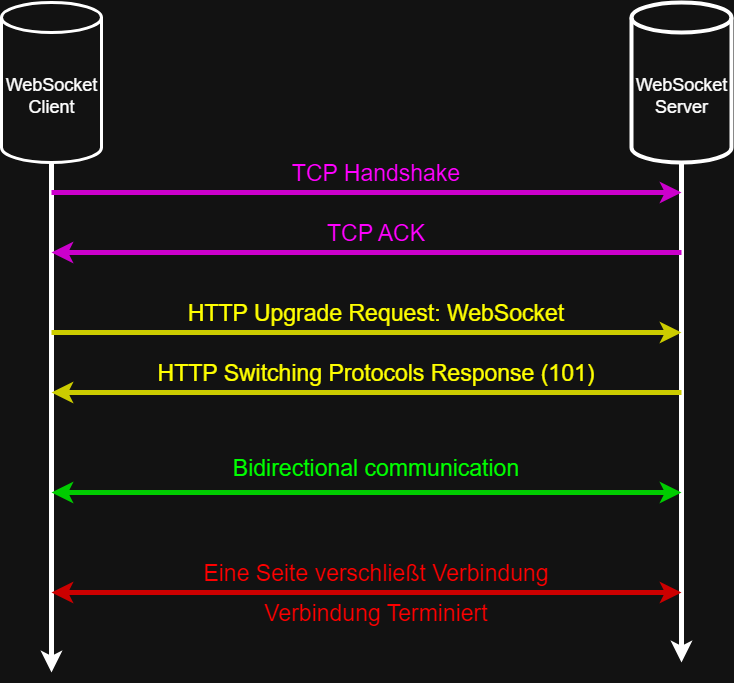
\includegraphics[width=\textwidth]{images/websocketflow.png}
  \end{minipage}
  \hspace{0.05\textwidth}
  \caption{WebSocket Communication Flow Diagram}
  \label{fig:WebSocket Flow Diagram}
\end{figure}
\vspace{1em}

{\large \textbf{Wie funktioniert WebSocket-Kommunikation?}}

Nach dem erfolgreichen Verbindungsaufbau ermöglicht WebSocket eine \textbf{vollständige bidirektionale Kommunikation} zwischen Client und Server. Das bedeutet, dass beide Seiten zu jeder Zeit Nachrichten senden und empfangen können – ohne wiederholte Anfragen oder Antwortzyklen wie bei HTTP.

Im Hintergrund basiert WebSocket auf dem \textbf{TCP/IP-Protokollstack} und nutzt die darunterliegenden Schichten des OSI-Modells zur Datenübertragung. Die folgende Tabelle zeigt, wie die einzelnen Schichten im Kontext einer WebSocket-Verbindung abgebildet werden:

\renewcommand{\arraystretch}{1.4} % More vertical spacing

% Define column types for better wrapping and alignment
\newcolumntype{Y}{>{\raggedright\arraybackslash}X}

\begin{table}[H]
\centering
\caption{OSI-Schichtenmodell am Beispiel einer WebSocket-Kommunikation}
\label{tab:websocket-osi}
\begin{tabularx}{\textwidth}{|l|Y|Y|}
\hline
\textbf{Schicht} & \textbf{Beschreibung} & \textbf{Zuständig} \\
\hline
7. Anwendung & Implementiert die WebSocket-Logik wie Senden und Empfangen von JSON-Nachrichten. & Ihre App (z.\,B. Qt WebSocket, Browser-JS) \\
\hline
6. Darstellung & Datenformatierung, z.\,B. JSON-Serialisierung oder ggf. Verschlüsselung. & Ihr Code (implizit) \\
\hline
5. Sitzung & Sitzungsmanagement, z.\,B. Wiederverbindung oder Ping/Pong-Mechanismen. & Ihre App oder Bibliotheken \\
\hline
4. Transport (TCP) & Zuverlässiger Transport, Flusskontrolle, Wiederholungen bei Paketverlust. & Betriebssystem (Kernel), Socket-Bibliotheken \\
\hline
3. Netzwerk (IP) & Routing und IP-Adressierung. & Betriebssystem (Kernel), Netzwerkstack \\
\hline
2. Sicherung (Ethernet/WLAN) & MAC-Adressierung, lokale Zustellung innerhalb des Netzwerks. & Netzwerkkartentreiber, Kernel \\
\hline
1. Physikalisch & Übertragung elektrischer oder funktechnischer Signale. & Hardware (z.\,B. NIC, Kabel, Antennen) \\
\hline
\end{tabularx}
\end{table}

\vspace*{1cm}
\begin{figure}[H]
  \centering
  \begin{minipage}[b]{0.82\textwidth}
    \centering
    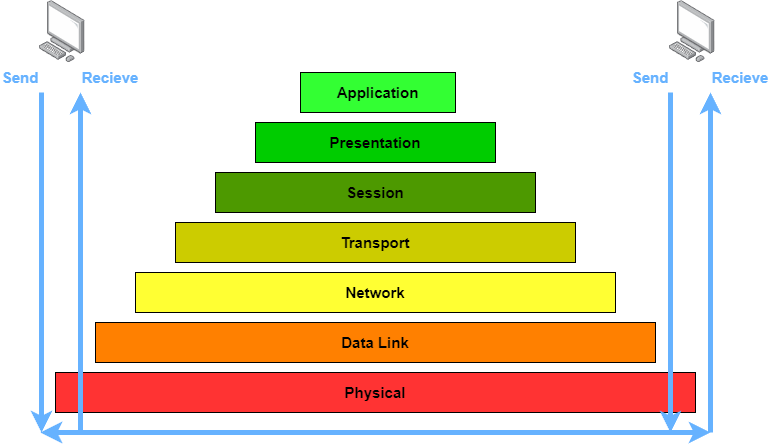
\includegraphics[width=\textwidth]{images/osi_works_01.png}
  \end{minipage}
  \hspace{0.05\textwidth}
  \caption{WebSocket Communication OSI-Modell}
  \label{fig:OSI-Modell}
\end{figure}
\vspace{1em}

\subsection*{Warum wurde WebSocket gewählt?}

Zur Anbindung externer Systeme an die KaVo-Dentaleinheit wurden verschiedene Kommunikationsprotokolle untersucht. Die folgende Tabelle bewertet relevante Kriterien hinsichtlich zentraler Anforderungen aus Stakeholder-Perspektive:

% Define column types for better wrapping and alignment
\newcolumntype{Y}{>{\raggedright\arraybackslash}X}

\begin{table}[H]
\centering
\caption{Vergleich möglicher Kommunikationsprotokolle}
\label{tab:kommunikationsvergleich}
\renewcommand{\arraystretch}{1.5}
\begin{tabularx}{\textwidth}{|Y|Y|Y|Y|}
\hline
\textbf{Kriterium} & \textbf{WebSocket} & \textbf{MQTT} & \textbf{HTTP (REST)} \\
\hline
Echtzeitfähigkeit &
\textcolor{green}{Sehr gut} &
\textcolor{green}{Sehr gut} &
\textcolor{red}{Begrenzt (Polling nötig)} \\
\hline
Bidirektionale Kommunikation &
\textcolor{green}{Ja} &
\textcolor{green}{Ja} &
\textcolor{red}{Nur Client → Server} \\
\hline
Standardisierbarkeit &
\textcolor{green}{\textit{RFC 6455 (IETF)}} &
\textcolor{green}{\textit{OASIS MQTT 5.0}} &
\textcolor{green}{\textit{RFC 2616 (HTTP/1.1)}} \\
\hline
Einfache Geräteerkennung (z.\,B. per mDNS) &
\textcolor{green}{Ja – mit Zeroconf nutzbar} &
\textcolor{red}{MQTT-Broker-basiert, kein mDNS} &
\textcolor{red}{Keine native Discovery} \\
\hline
Offline-Betrieb möglich &
\textcolor{green}{Ja} &
\textcolor{green}{Ja – lokaler Broker} &
\textcolor{green}{Ja – lokal betreibbar} \\
\hline
Kompatibilität mit Home Assistant oder ähnlich &
\textcolor{green}{Sehr gut (Custom Integration)} &
\textcolor{green}{Native Unterstützung} &
\textcolor{green}{Möglich mit REST-Sensor} \\
\hline
Integration in externe Lösungen &
\textcolor{green}{Sehr flexibel} &
\textcolor{red}{MQTT-Broker- und Topic-Struktur nötig} &
\textcolor{green}{Einfach per HTTP-Client} \\
\hline
Infrastrukturaufwand &
\textcolor{green}{Gering – nur Server nötig} &
\textcolor{red}{Höher – Broker + Verwaltung} &
\textcolor{green}{Minimal (z.\,B. Flask)} \\
\hline
Kompatibilität mit \textit{CONNECTbase}-Softwarearchitektur &
\textcolor{green}{Sehr gut – native Qt-Unterstützung vorhanden} &
\textcolor{red}{Nur über externe MQTT-Bibliotheken integrierbar} &
\textcolor{green}{Möglich über Qt HTTP-Module, aber unidirektional} \\
\hline
\end{tabularx}
\end{table}
\vspace{1em}
\noindent
Auf Basis der in Tabelle~\ref{tab:kommunikationsvergleich} dargestellten Kriterien wurde \textbf{WebSocket} als bevorzugte Lösung gewählt. Es erfüllt sämtliche funktionalen und nicht-funktionalen Anforderungen der Stakeholder – insbesondere im Hinblick auf Echtzeitfähigkeit, bidirektionale Kommunikation, Standardisierbarkeit sowie eine nahtlose Integration in die bestehende \textit{CONNECTbase}-Softwarearchitektur und externe Lösungen.

\subsubsection{QMdnsEngine}

\textbf{QMdnsEngine} ist eine externe, \textbf{Open-Source}-C++-Bibliothek, die unter der \textbf{MIT-Lizenz} auf GitHub: {\url{https://github.com/nitroshare/qmdnsengine}} veröffentlicht wurde. Sie wurde speziell dafür entwickelt, das \textbf{Multicast DNS (mDNS)}-Protokoll sowie grundlegende \textbf{Zeroconf-Funktionalität} innerhalb von \textbf{Qt}-Anwendungen zu implementieren. 

Im Gegensatz zu anderen mDNS-Implementierungen wie \textit{Avahi} oder \textit{Bonjour}, die externe Daemons benötigen, ist \textit{QMdnsEngine} vollständig in Qt integriert. Dadurch eignet sie sich ideal für eingebettete Systeme wie die \textit{KaVo-Dentaleinheit}, auf der auch die Software \textit{CONNECTbase} basiert.

Die Bibliothek ermöglicht es einem Gerät, sich im lokalen Netzwerk automatisch bekannt zu machen – ohne zentrale DNS- oder DHCP-Server. Dabei kann ein Dienst wie folgt angekündigt werden:

\begin{quote}
„Ich biete einen Dienst \texttt{\_kavochair.\_tcp.local} auf Port \texttt{8080} mit dem Namen \texttt{KaVo-TC-1} an -- erreichbar unter meiner IPv4- und/oder IPv6-Adresse.“
\end{quote}

\textit{QMdnsEngine} unterstützt sowohl IPv4- als auch IPv6-Adressen und übernimmt die automatische Erzeugung sowie Beantwortung von DNS-Nachrichten über Multicast. Dies bildet die Basis für eine vollständig dezentrale Geräteerkennung und Dienstveröffentlichung im lokalen Netzwerk – ganz ohne Konfigurationsaufwand.

Diese Fähigkeit zur \textbf{automatischen Entdeckung} ist besonders relevant im Hinblick auf die zukünftige Verwendung des WebSocket-Endpunkts: Sobald der Dienst veröffentlicht wurde, kann eine Plattform wie \textit{Home Assistant} ihn automatisch finden und integrieren – \textbf{ohne manuelle IP-Konfiguration}. Dadurch wird die Nutzung für Endanwender deutlich robuster, komfortabler und fehlertoleranter.


\subsubsection{JSON}

\textbf{JSON (JavaScript Object Notation)} ist ein leichtgewichtiges, textbasiertes Datenformat zur strukturierten Darstellung von Informationen. Es wurde ursprünglich für JavaScript entwickelt, ist heute jedoch unabhängig von Programmiersprachen und hat sich als De-facto-Standard für den Datenaustausch zwischen Systemen etabliert.

JSON stellt Daten in Form von Schlüssel-Wert-Paaren dar und ist sowohl für Maschinen als auch für Menschen leicht lesbar. Ein typisches JSON-Objekt könnte wie folgt aussehen:

\begin{lstlisting}[language=json,caption={Beispiel für ein JSON-Objekt},label={lst:json-example}]
{
  "Error_message": "Disinfektionsmittel leer",
  "Hygiene_plan_type": "Nach Behandlung",
  "Hygiene_plan_phase": "Phase 1"
}
\end{lstlisting}

\textbf{Warum JSON?} 

In dieser Arbeit dient JSON als Austauschformat für die Kommunikation über WebSockets – z.\,B. zwischen der \textit{CONNECTbase-Testumgebung} und einer \textit{Home Assistant}-Instanz. Die Gründe für den Einsatz von JSON sind:

\begin{itemize}
  \item \textbf{Einfachheit:} JSON ist kompakt, leicht zu generieren und zu parsen – insbesondere mit der in Qt enthaltenen Klasse \texttt{QJsonDocument}.\\
  \item \textbf{Kompatibilität:} JSON ist in nahezu jeder Programmiersprache verfügbar und wird von vielen Plattformen (z.\,B. Home Assistant, Webbrowsern, Node-RED) nativ unterstützt.\\
  \item \textbf{Flexibilität:} Die Struktur lässt sich leicht erweitern, etwa durch zusätzliche Felder zur Beschreibung neuer Zustände oder Parameter.\\
  \item \textbf{Lesbarkeit:} Selbst ohne spezielle Tools lässt sich der Inhalt eines JSON-Dokuments gut nachvollziehen und debuggen.\\
  \item \textbf{Netzwerkfähigkeit:} Nur als \textit{String} (nicht als internes Objekt) kann ein JSON-Inhalt über das Netzwerk gesendet werden. In Qt wird dazu ein \texttt{QJsonObject} mittels \texttt{QJsonDocument} in einen kompakten \texttt{QString} serialisiert, der anschließend per WebSocket verschickt werden kann.
\end{itemize}

\textbf{Serialisierung in Qt:}

Ein \texttt{QJsonObject} stellt eine strukturierte Datenmenge in Qt dar. Um diese über das Netzwerk zu übertragen, wird sie folgendermaßen in einen String umgewandelt:

\begin{lstlisting}[language=C++,caption={Serialisierung eines JSON-Objekts in Qt},label={lst:json-qt}]
QJsonObject obj;
obj["hygiene_plan_type"] = "Wochentlich";

QJsonDocument doc(obj);
QString jsonString = doc.toJson(QJsonDocument::Compact);
\end{lstlisting}

Durch diese Kombination aus Struktur (Objekt), Serialisierung (Dokument) und Übertragung (String) wird eine robuste, erweiterbare und plattformunabhängige Kommunikation zwischen der Dentaleinheit und externen Systemen realisiert.


\subsection{Wie wurde die Übertragung technisch umgesetzt?}

\subsubsection{Qt GUI}

Zur Simulation der Datenausgabe einer echten Dentaleinheit wurde eine eigene \textbf{Qt-Widget-Oberfläche} entwickelt. Diese grafische Benutzeroberfläche dient als kontrollierbare Testumgebung und bildet typische Ausgangsdaten eines Behandlungsstuhls ab – etwa Sensorzustände, Fehlerstatus und Hygieneprogramme. Sie ermöglicht eine praxisnahe Verifikation der Schnittstelle ohne Zugriff auf ein echtes Gerät.

\begin{figure}[H]
  \centering
  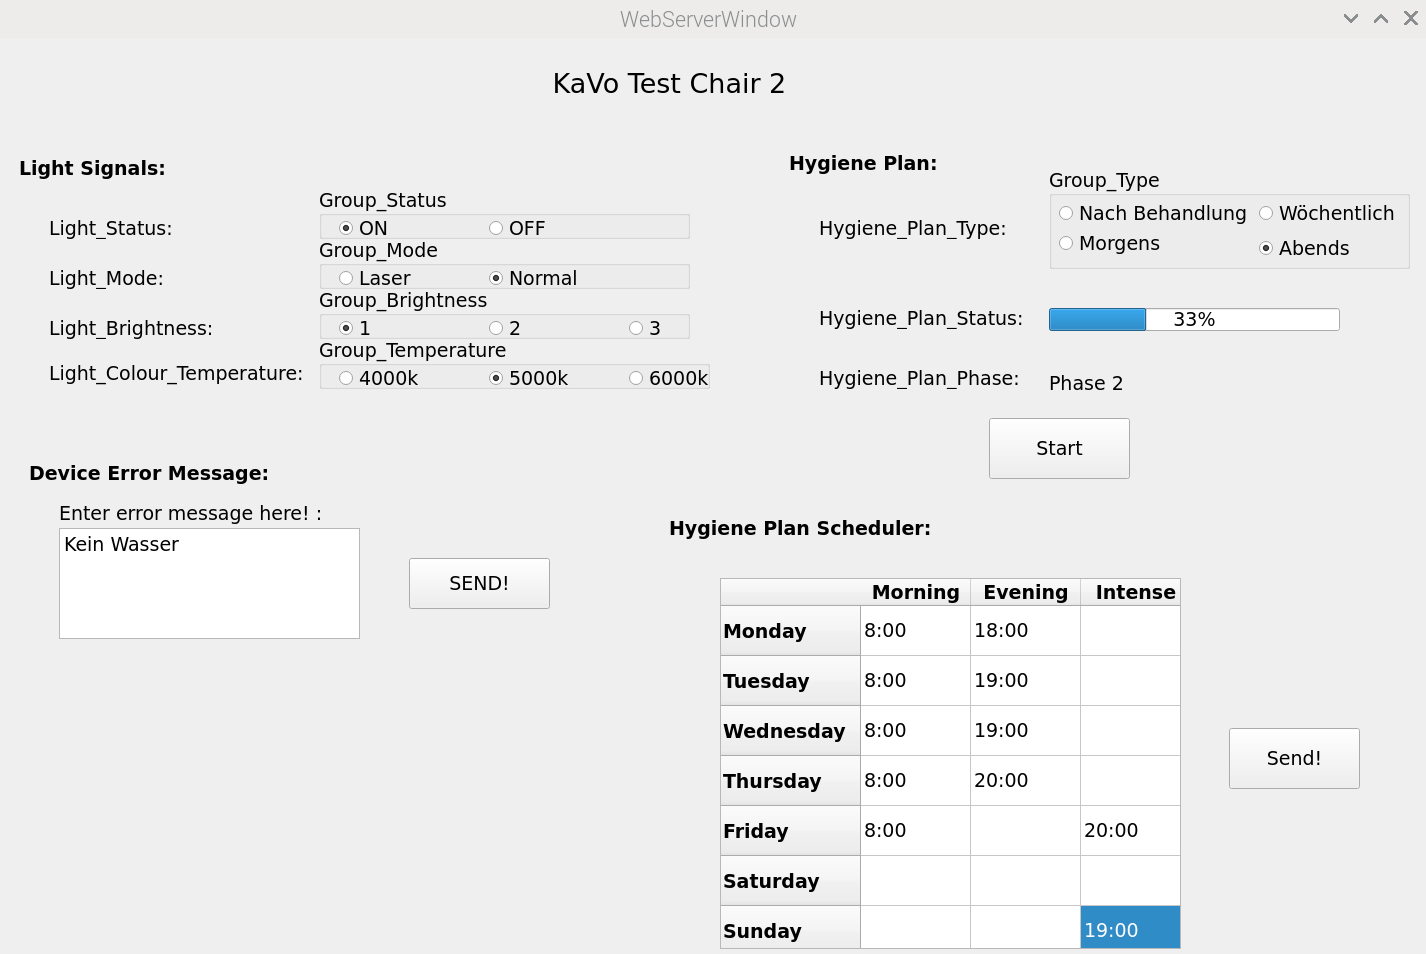
\includegraphics[width=1\textwidth]{images/guifin1.png}
  \caption{Test-GUI zur Simulation einer KaVo-Dentaleinheit}
  \label{fig:Qt-GUI}
\end{figure}

Die grafische Oberfläche adressiert zentrale Anwendungsfälle, die in den Stakeholder-Stories beschrieben wurden:

\begin{itemize}
  \item \textbf{Light Signals:} Die Lichtparameter (Status, Modus, Helligkeit, Farbtemperatur) repräsentieren den Zustand der Lichtkomponente der Dentaleinheit. Sie dienen als Beispiel für die Übermittlung und Visualisierung von Gerätezuständen – etwa zur Anzeige im Frontend oder zur Diagnose durch externe Systeme.\\
  
  \item \textbf{Device Error Message:} Über ein Texteingabefeld kann eine Fehlermeldung simuliert und übertragen werden – analog zu Fehlerprotokollen, die Servicetechnikern zur Verfügung stehen sollen.\\
  
  \item \textbf{Hygiene Plan:} Visualisiert wird nicht nur der Fortschritt über einen Balken, sondern es werden auch der \textit{Hygieneplan-Typ} (z.\,B. „Morgens“, „Abends“) und die \textit{aktuelle Phase} übertragen. Diese Daten bilden die Grundlage für Automatisierungen – z.\,B. automatisches Ausschalten nur bei bestimmten Plänen (Abends, Wöchentlich).\\
  
  \item \textbf{Hygiene Plan Scheduler:} Über eine Tabelle können geplante Startzeiten für jeden Wochentag konfiguriert werden. Diese dienen der externen Automatisierung – etwa dem automatischen Einschalten vor Beginn des Programms.
\end{itemize}


\textbf{\large Sende-Buttons und Nachrichtenlogik:}

Jeder Datenbereich der GUI ist mit einem separaten \textbf{„Send/Start“-Button} verknüpft. Wird dieser betätigt, werden die konfigurierten Werte als strukturierte JSON-Nachricht an den WebSocket-Server übergeben – ähnlich wie CONNECTbase relevante Statusdaten selektiv an externe Systeme weitergibt.

\begin{itemize}
  \item Der Button für \textbf{Licht und Fehlermeldung} sendet aktuelle Lichtparameter und die eingegebene Fehlermeldung.\\
  \item Der Button für den \textbf{Hygieneplan} überträgt Plan-Typ, Phase, Fortschritt und Abschlusszeitpunkt.\\
  \item Der Button für den \textbf{Hygieneplan-Scheduler} sendet den vollständigen Wochenplan für automatische Abläufe.
\end{itemize}

Diese \textbf{modulare Nachrichtenlogik} erlaubt das gezielte Testen einzelner Anwendungsfälle und bildet die segmentierte Zustandsübermittlung produktiver Systeme realitätsnah ab. Alle JSON-Nachrichten wurden direkt über die \texttt{sendJson()}-Methode des Servers an verbundene Clients gesendet.\\\\

\textbf{Beispielhafte JSON-Ausgaben:}


\begin{lstlisting}[language=json,caption={Lichtstatus und Fehlermeldung},label={lst:json-light}]
{
  "error_message": "Kein Wasser",
  "light_brightness": "1",
  "light_mode": "Normal Mode",
  "light_status": "ON",
  "light_temperature": "5000k"
}
\end{lstlisting}

\begin{lstlisting}[language=json,caption={Dynamische Hygieneplan-Daten},label={lst:json-hygiene}]
{ "hygiene_plan_type": "Evening" }
{ "hygiene_plan_phase": "Phase 3", "hygiene_plan_progress": "99" }
{ "hygiene_plan_phase": "Phase 3", "hygiene_plan_progress": "100" }
{ 
  "hygiene_plan_done_at": "2025-07-15T13:32:40", 
  "hygiene_plan_phase": "Evening Hygiene process completed" 
}
\end{lstlisting}

\begin{lstlisting}[language=json,caption={Geplanter Hygienezeitplan (Wochentage)},label={lst:json-calendar}]
{
  "CAL_monday_morning": "2025-07-21T08:00:00",
  "CAL_monday_evening": "2025-07-21T18:00:00",
  "CAL_tuesday_morning": "2025-07-15T08:00:00",
  "CAL_tuesday_evening": "2025-07-15T19:00:00",
  "CAL_wednesday_morning": "2025-07-16T08:00:00",
  "CAL_wednesday_evening": "2025-07-16T19:00:00",
  "CAL_thursday_morning": "2025-07-17T08:00:00",
  "CAL_thursday_evening": "2025-07-17T20:00:00",
  "CAL_friday_morning": "2025-07-18T08:00:00",
  "CAL_friday_intense": "2025-07-18T20:00:00",
  "CAL_sunday_intense": "2025-07-20T19:00:00"
}
\end{lstlisting}

\noindent Die oben dargestellten Nachrichten veranschaulichen die praktische Umsetzung der geplanten Übertragungsschnittstelle und zeigen, wie sich unterschiedliche Statusinformationen getrennt übertragen und gezielt verarbeiten lassen – etwa zur Visualisierung oder Automatisierung in Home Assistant.

\vspace{1cm}
\textbf{\large Qt GUI Projekt struktur:} 

\begin{figure}[H]
\centering
\begin{minipage}{0.75\textwidth}
\begin{itemize}
  \item \textbf{projekt/}
  \begin{itemize}
    \item CMakeLists.txt
    \item \textbf{Header-Dateien/}
    \begin{itemize}
      \item webserverwindow.h
      \item Qmdns.h
    \end{itemize}
    \item \textbf{Quellcode-Dateien/}
    \begin{itemize}
      \item main.cpp
      \item webserverwindow.cpp
      \item Qmdns.cpp
    \end{itemize}
    \item \textbf{UI-Dateien/}
    \begin{itemize}
      \item webserverwindow.ui
    \end{itemize}
    \item \textbf{external/}
    \begin{itemize}
      \item QMdnsEngine/
    \end{itemize}
  \end{itemize}
\end{itemize}
\end{minipage}
\caption{Projektstruktur der Testumgebung mit \textit{WebSocket}-Server und \textit{QMdnsEngine}}
\label{fig:projektstruktur}
\end{figure}
\vspace{1cm}
\textbf{\large Die technische Umsetzung der Datenübertragung basiert auf drei wesentlichen Komponenten:} 
\begin{enumerate}
  \item der Integration der Bibliothek \textbf{QMdnsEngine}, die eine automatische 
  Dienstveröffentlichung im lokalen Netzwerk ermöglicht.\\
  \item einem \textbf{WebSocket-Server}, der eine persistente Verbindung zu externen Clients (z.\,B. Home Assistant) herstellt.\\
  \item der \textbf{JSON-Datenstruktur}, mit der die Nachrichten übertragen werden.
\end{enumerate}

\vspace{1em}
\subsubsection{QMdnsEngine Implementierung}

Für die automatische Erkennung der Dentaleinheit im lokalen Netzwerk wurde die Open-Source-Bibliothek \texttt{QMdnsEngine} integriert. Diese wurde im Projekt als Unterverzeichnis \texttt{external/QMdnsEngine} eingebunden und über \texttt{add\_subdirectory()} in der \texttt{CMakeLists.txt} registriert:
\vspace{1cm}
\begin{lstlisting}[language=bash,caption={Einbindung der QMdnsEngine in das Projekt},label={lst:cmake-qmdns}]
# QMdnsEngine einbinden
add_subdirectory(external/QMdnsEngine)

# Link gegen die Bibliothek
target_link_libraries(test_webserver PRIVATE
    Qt6::Core
    Qt6::Network
    Qt6::WebSockets
    Qt6::Widgets
    qmdnsengine
)
\end{lstlisting}
\vspace{1cm}
Die Initialisierung und Veröffentlichung des Dienstes erfolgt über eine eigene Klasse \texttt{MdnsPublisher}, die den Dienst mit Namen, Port und Metadaten im Netzwerk sichtbar macht. Ein besonders wichtiger Teil hierbei ist die Definition des \textbf{Service Type}, der darüber entscheidet, wie und von welchen Clients der Dienst erkannt werden kann. In diesem Projekt wurde der Service Type explizit auf:

\begin{center}
\texttt{\_kavochair.\_tcp.local.}
\end{center}

gesetzt, um eine automatische Erkennung durch Home Assistant und ähnliche Systeme zu ermöglichen. Dieser Wert wird in der Methode \texttt{publish()} des \texttt{MdnsPublisher}-Objekts gesetzt:
\vspace{1cm}
\begin{lstlisting}[language=c++,caption={mDNS-Dienst mit QMdnsEngine veröffentlichen},label={lst:qmdns-publish}]
MdnsPublisher mdns;
QMap<QString, QString> txt = {
    {"manufacturer", "KaVo"},
    {"model", "Testerchair"},
    {"version", "1.0.1"}
};
mdns.publish("KaVo TC 2", 8090, txt);

// Intern in der Methode:
m_service.setType("_kavochair._tcp.local.");
\end{lstlisting}
\vspace{1cm}
\textbf{Dabei wird ein Dienst wie folgt angekündigt:}

\begin{quote}
„Ich biete einen Dienst \texttt{\_kavochair.\_tcp.local} auf Port \texttt{8090} mit dem Namen \texttt{KaVo TC 2} an – erreichbar unter meiner IPv4- und/oder IPv6-Adresse.“
\end{quote}

\vspace{0.5cm}
Früher wurde der mDNS-Dienst alle \textbf{30 Sekunden erneut angekündigt}, um für neu hinzukommende Geräte im Netzwerk sichtbar zu bleiben. Dies geschah unabhängig vom tatsächlichen Nutzungsstatus. Um jedoch unnötigen Netzwerkverkehr zu vermeiden, wurde das Verhalten angepasst:

\textbf{Die Wiederankündigung erfolgt nun nur noch, wenn keine WebSocket-Clients verbunden sind.}

Sobald ein Client verbunden ist, wird der \texttt{QTimer} gestoppt. Wenn alle Clients wieder getrennt sind, wird die periodische Ankündigung automatisch erneut aktiviert:
\vspace{1cm}
\begin{lstlisting}[language=c++,caption={mDNS-Wiederankündigung nur bei Inaktivität},label={lst:qmdns-conditional}]
connect(&m_announceTimer, &QTimer::timeout, this, [this]() {
    m_provider->update(m_service);
    qDebug() << "Re-announcing service: " << m_service.name();
});

// Nur starten, wenn keine Clients aktiv sind
void MdnsPublisher::startReannounce() {
    if (!m_announceTimer.isActive()) {
        m_announceTimer.start(30000);
    }
}

// Timer stoppen, wenn ein Client verbunden ist
void MdnsPublisher::stopReannounce() {
    if (m_announceTimer.isActive()) {
        m_announceTimer.stop();
    }
}
\end{lstlisting}
Die Verbindung zwischen WebSocket-Clientstatus und mDNS-Ankündigung erfolgt über ein Signal-slot-System zwischen dem Serverfenster und dem \texttt{MdnsPublisher}.\\

\vspace{0.5cm}
\textbf{Warum ist das wichtig?}\\ 
Dadurch bleibt die Behandlungseinheit im Netzwerk kontinuierlich auffindbar – selbst wenn sich Clients (wie z.\,B. \textit{Home Assistant}) zu einem späteren Zeitpunkt verbinden oder Netzwerkinformationen zwischendurch verloren gehen. Der Dienst ist so jederzeit erreichbar.

Damit externe Clients den WebSocket-Server auch wirklich unter der vom mDNS-Dienst angekündigten Adresse erreichen können, wurde der Server auf \texttt{QHostAddress::Any} gebunden. Das bedeutet:

\begin{itemize}
  \item Der Server akzeptiert Verbindungen über \texttt{LAN (eth0)}, \texttt{WLAN (wlan0)} oder \texttt{localhost}.\\
  \item Er ist automatisch kompatibel mit der IP-Adresse, die vom mDNS-Dienst ausgestrahlt wird.
\end{itemize}

Diese Kombination stellt sicher, dass externe Plattformen wie \textit{Home Assistant} den WebSocket-Endpunkt jederzeit zuverlässig finden und erreichen können – unabhängig vom verwendeten Netzwerkinterface der Dentaleinheit.



\subsubsection{WebSocket-Server: Implementierung}

In der Datei \texttt{webserverwindow.cpp} wurde ein \texttt{QWebSocketServer} initialisiert, der auf Port \texttt{8090} lauscht und neue Verbindungen akzeptiert:

\begin{lstlisting}[language=c++,caption={Initialisierung des WebSocket-Servers},label={lst:websocket-server}]
webSocketServer = new QWebSocketServer(QStringLiteral("Test Server"),
                        QWebSocketServer::NonSecureMode, this);

if (webSocketServer->listen(QHostAddress::Any, 8090)) {
    connect(webSocketServer, &QWebSocketServer::newConnection,
            this, &WebServerWindow::onNewConnection);
}
\end{lstlisting}

Neue Clients werden über die Methode \texttt{onNewConnection()} angenommen. Direkt nach dem Verbindungsaufbau wird ein Initialpaket mit Standardwerten an den Client gesendet.

Je nachdem, welcher \texttt{send}-Button im GUI gedrückt wird (z.\,B. \texttt{Send Hygiene}, \texttt{Send Status}, etc.), wird ein entsprechendes Datenpaket erzeugt, in ein kompaktes JSON-Format umgewandelt und über die WebSocket-Verbindung an alle aktuell verbundenen Clients gesendet.

\vspace{1em}
\subsubsection{JSON-Verarbeitung und Nachrichtenübertragung}

Zur Datenübertragung wurde das Format \texttt{JSON} verwendet. Die Methode \texttt{sendJson()} nimmt ein \texttt{QJsonObject}, wandelt es in einen kompakten \texttt{QString} um und überträgt es an alle verbundenen Clients:

\begin{lstlisting}[language=c++,caption={Versand strukturierter JSON-Nachrichten},label={lst:send-json}]
void WebServerWindow::sendJson(const QJsonObject &data) {
    QJsonDocument doc(data);
    QString jsonString = doc.toJson(QJsonDocument::Compact);
    for (QWebSocket *client : clients) {
        client->sendTextMessage(jsonString);
    }
}
\end{lstlisting}

\vspace{1em}
\subsubsection{Fazit}

Durch die Kombination aus Qt-Widget-Oberfläche, WebSocket-Kommunikation, strukturierter JSON-Nachrichtenübertragung und automatischer Dienstveröffentlichung via QMdnsEngine wurde eine vollständig kompatible, netzwerkfähige und leicht erweiterbare Testumgebung geschaffen. Diese bildet die zentrale Grundlage für die spätere Integration mit Home Assistant und simuliert realitätsnah die Verhaltensweise einer echten \textit{KaVo-Dentaleinheit}.

\section{Externe Automatisierungs- und Visualisierungsplattform}
\subsection{Home Assistant}

Home Assistant ist eine Open Source, lokal betriebene Plattform für Heimautomatisierung, die 2013 von Paulus Schoutsen initiiert wurde und heute von der \textit{Open Home Foundation} gepflegt wird. Ziel der Plattform ist es, verschiedenste smarte Geräte und Dienste in einem einheitlichen System zu integrieren und automatisiert zu steuern – ganz ohne Cloud-Abhängigkeit.

Die Plattform läuft typischerweise auf einem Einplatinencomputer wie dem \textit{Raspberry Pi} oder auf dedizierter Hardware wie \textit{Home Assistant Yellow}. Über eine intuitive Weboberfläche oder mobile Apps (Android/iOS) können Nutzer:innen ihr Smart Home konfigurieren und steuern. Sprachsteuerung über \textit{Google Assistant}, \textit{Amazon Alexa} oder \textit{Apple Siri} sowie Home Assistants eigene \textit{Assist}-Funktionalität wird ebenfalls unterstützt.

Im Zentrum des Konzepts steht der lokale Datenschutz: Daten bleiben im eigenen Netzwerk, und Cloud-Dienste werden nur genutzt, wenn keine lokale API zur Verfügung steht. Diese Philosophie sowie die große Community machen Home Assistant zu einem der aktivsten Open-Source-Projekte weltweit.

\subsubsection{Home Assistant Architektur}

Die Architektur von Home Assistant ist modular aufgebaut und besteht aus mehreren Schichten, die zusammen eine flexible, erweiterbare und lokal betriebene Smart-Home-Plattform ermöglichen. Die wesentlichen Komponenten sind:

\begin{itemize}
  \item \textbf{Home Assistant Core:} Der zentrale Anwendungskern ist in Python geschrieben und bildet das Herzstück des Systems. Er stellt die Integrations- und Automatisierungslogik bereit und verwaltet die Kommunikation mit den angebundenen Geräten über sogenannte Integrationen. Der Core betreibt einen internen Ereignisbus, eine Zustandsmaschine sowie einen Serviceregistrar zur Steuerung aller verbundenen Geräte.\\
  
  \item \textbf{Supervisor:} Der Supervisor ist ein Verwaltungsdienst, der für die Installation, Aktualisierung und Wartung von Home Assistant sowie dessen Add-ons zuständig ist. Er ermöglicht automatische Backups, überwacht den Systemzustand und verwaltet die Container-Umgebung. Zudem stellt er einheitliche Schnittstellen für Audio, DNS und mDNS zur Verfügung.\\

  \item \textbf{Home Assistant OS:} Ein schlankes, auf Linux basierendes Betriebssystem, das speziell für Home Assistant entwickelt wurde. Es beinhaltet Docker zur Containerisierung aller Komponenten und nutzt D-Bus zur Kommunikation mit dem System (z.~B. Netzwerkverwaltung). Es ermöglicht ein konsistentes und wartungsarmes Smart-Home-System auf dedizierter Hardware.

\end{itemize}

\vspace*{1cm}
\begin{figure}[H]
  \centering
  \begin{minipage}[b]{0.82\textwidth}
    \centering
    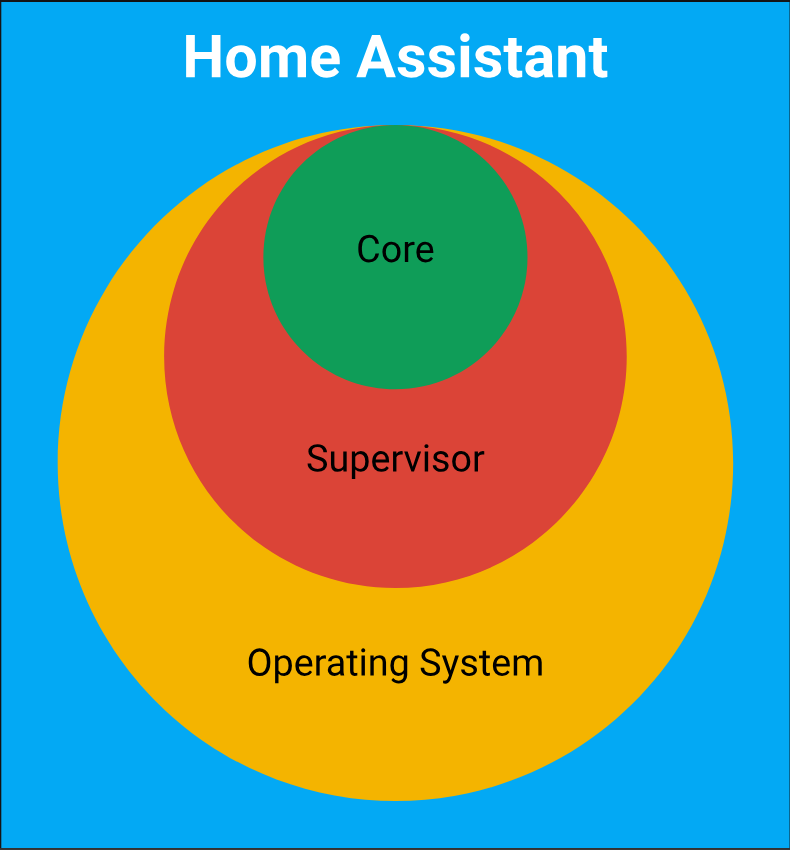
\includegraphics[width=\textwidth]{images/HA_Architecture.png}
  \end{minipage}
  \hspace{0.05\textwidth}
  \caption{Home Assistant Architektur}
  \label{fig:OSI-Modell}
\end{figure}
\vspace{1em}

\noindent
Diese Architektur erlaubt es, Home Assistant auf verschiedene Weise zu betreiben:
\begin{itemize}
  \item \textbf{Home Assistant OS:} Komplette Installation mit Supervisor, Core und OS.\\
  \item \textbf{Home Assistant Supervised:} Supervisor und Core laufen auf einem bestehenden Linux-System.\\
  \item \textbf{Home Assistant Container:} Nur der Core läuft in einem Docker-Container ohne Supervisor.\\
  \item \textbf{Home Assistant Core:} Nur das Python-Programm wird direkt installiert.
\end{itemize}

\vspace{0.5em}
\noindent
Die Komponenten arbeiten eventbasiert: Änderungen an Geräten oder Zuständen lösen Ereignisse auf dem internen Bus aus, welche dann von Automationen, Benutzeroberflächen oder anderen Integrationen verarbeitet werden können. Diese lose Kopplung ermöglicht eine hohe Modularität und Erweiterbarkeit.

\subsubsection{Home Assistant Core}

\begin{figure}[H]
  \centering
  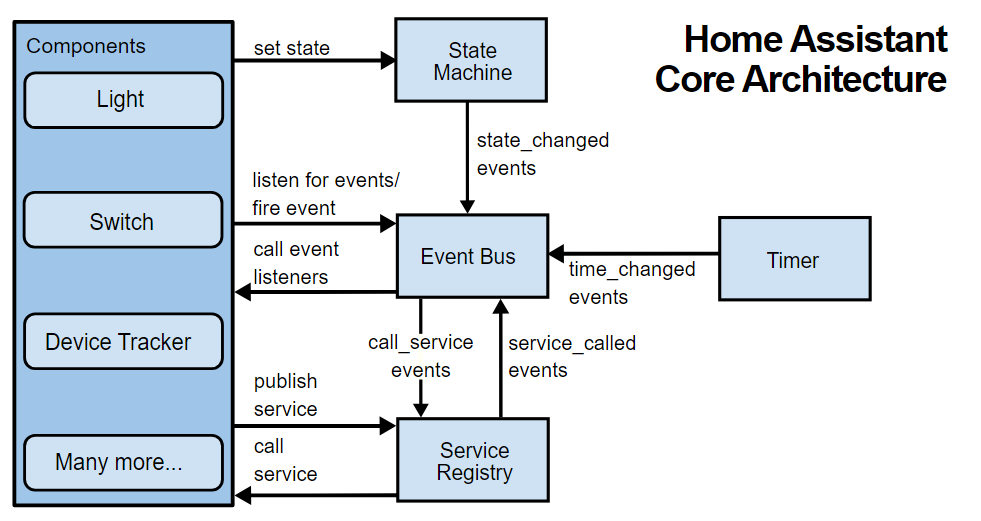
\includegraphics[width=0.85\textwidth]{images/HA_core_architechture.png}
  \caption{Architektur des Home Assistant Core}
  \label{fig:ha-core-architecture}
\end{figure}
\vspace{0.5em}

Der \textit{Home Assistant Core} bildet die logische Zentrale der Plattform. Er ist in Python geschrieben und stellt grundlegende Mechanismen zur Verfügung, über die alle Integrationen, Entitäten und Automatisierungen miteinander kommunizieren. Die Architektur folgt einem entkoppelten, ereignisbasierten Modell, das eine hohe Flexibilität und Erweiterbarkeit ermöglicht. Der Kern besteht aus vier Hauptkomponenten:

\begin{itemize}
  \item \textbf{Event Bus:} Der Ereignisbus ist das zentrale Kommunikationssystem innerhalb von Home Assistant. Alle Komponenten und Integrationen können Ereignisse auf diesem Bus senden oder abonnieren. Typische Ereignisse sind beispielsweise \texttt{state\_changed}, \texttt{call\_service} oder benutzerdefinierte Ereignisse. Der Event Bus ermöglicht eine lose Kopplung zwischen Komponenten und ist somit das ``schlagende Herz'' des Systems.\\

  \item \textbf{State Machine:} Die Zustandsmaschine verwaltet den aktuellen Zustand aller registrierten Entitäten. Jeder Zustand wird mit einer eindeutigen ID (z.\,B. \texttt{light.kitchen}) und optionalen Attributen gespeichert. Bei jeder Änderung wird automatisch ein \texttt{state\_changed}-Ereignis auf dem Event Bus ausgelöst, sodass andere Komponenten auf diese Änderung reagieren können.\\

  \item \textbf{Service Registry:} Die Serviceregistrierung erlaubt es, systemweit Dienste bereitzustellen und aufzurufen. Wenn ein Nutzer oder eine Automation z.\,B. \texttt{light.turn\_on} aufruft, wird intern ein \texttt{call\_service}-Ereignis generiert. Der Service-Handler ruft anschließend die entsprechende Funktion in der zuständigen Integration auf. Neue Dienste können durch Integrationen registriert werden und stehen dann für Automatisierungen zur Verfügung.\\

  \item \textbf{Timer:} Der Timer sendet jede Sekunde ein \texttt{time\_changed}-Ereignis auf dem Event Bus. Dadurch können zeitbasierte Automatisierungen und periodische Aktualisierungen von Entitäten realisiert werden. Der Timer ist essenziell für Uhrzeit-getriggerte Logik innerhalb von Home Assistant.
\end{itemize}

\noindent
Zusätzlich zu diesen Hauptkomponenten stellt der Core zahlreiche Hilfsklassen bereit, etwa zur Entitätsverwaltung, Standortverarbeitung oder Gerätekonfiguration. Alle Interaktionen innerhalb des Systems basieren auf dem Austausch von Ereignissen und Zustandsänderungen – dies ermöglicht ein entkoppeltes und reaktionsfähiges Smart-Home-System.

\subsubsection{Home Assistant Supervisor}

Der \textit{Home Assistant Supervisor} ist eine zentrale Verwaltungsinstanz innerhalb des Home Assistant-Ökosystems. Er erweitert die Core-Funktionalität um Systemmanagement, Softwarewartung und Add-on-Verwaltung. Der Supervisor läuft in einem eigenen Docker-Container und übernimmt dabei verschiedene administrative Aufgaben, die normalerweise manuell durchgeführt werden müssten.

\vspace{0.5em}
\noindent
Die Hauptverantwortlichkeiten des Supervisors sind:

\begin{itemize}
  \item Starten und Überwachen von \textbf{Home Assistant Core}.\\
  \item Durchführen von \textbf{Updates} der Core-Instanz (inkl. automatischer Zurücksetzung bei Fehlern).\\
  \item Erstellen und Wiederherstellen von \textbf{Backups (Snapshots)}.\\
  \item Verwaltung von \textbf{Add-ons} (z.\,B. MQTT-Broker, Node-RED, Samba, Visual Studio Code).\\
  \item Bereitstellung eines \textbf{einheitlichen Audio-Subsystems} für Core und Add-ons.\\
  \item Durchführung von Betriebssystem-Updates (bei Verwendung von Home Assistant OS).
\end{itemize}

\vspace{0.5em}
\noindent
Die Architektur des Supervisors basiert auf einer containerisierten Umgebung mit mehreren voneinander isolierten Komponenten, die über definierte Schnittstellen miteinander kommunizieren. Abbildung~\ref{fig:ha-supervisor-architecture} veranschaulicht die Systemarchitektur.

\begin{figure}[H]
  \centering
  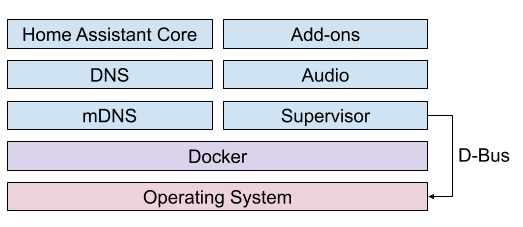
\includegraphics[width=0.85\textwidth]{images/HA_supervisor_architecture.png}
  \caption{Architektur des Home Assistant Supervisors}
  \label{fig:ha-supervisor-architecture}
\end{figure}

\noindent
\textbf{Die wichtigsten Bestandteile der Architektur sind:}

\begin{itemize}
  \item \textbf{Home Assistant Core:} Die zentrale Automatisierungsplattform zur Verwaltung von Integrationen, Entitäten und Automationen.\\
  \item \textbf{Add-ons:} Isolierte Zusatzanwendungen, die in eigenen Containern laufen und dem System zusätzliche Funktionen bereitstellen.\\
  \item \textbf{DNS-Server:} Erlaubt die interne Kommunikation zwischen Home Assistant Core und Add-ons über Netzwerkaliase.\\
  \item \textbf{Audio-System:} Einheitliche Infrastruktur zur Audioübertragung zwischen Core und Add-ons.\\
  \item \textbf{mDNS:} Ermöglicht die automatische Erkennung von Geräten und Diensten im lokalen Netzwerk.\\
  \item \textbf{Supervisor:} Verwalter aller Systemkomponenten, mit Verantwortung für Updates, Konfiguration und Orchestrierung.\\
  \item \textbf{Docker:} Container-Engine zur Isolation und Verwaltung aller Home Assistant-Komponenten.\\
  \item \textbf{Operating System:} Ein schlankes Linux-basiertes Betriebssystem, das speziell für Home Assistant entwickelt wurde (z.\,B. Home Assistant OS).\\
  \item \textbf{D-Bus:} Interprozesskommunikation zwischen dem Betriebssystem und Systemdiensten, etwa zur Steuerung des Netzwerkmanagers.
\end{itemize}

\vspace{0.5em}
\noindent
Durch diese modulare Container-Architektur bleibt das System erweiterbar, fehlertolerant und gleichzeitig einfach zu verwalten. Der Supervisor bildet somit die Grundlage für eine nutzerfreundliche und wartbare Home Assistant-Installation.

\subsubsection{Home Assistant Operating System (HAOS)}

Das \textbf{Home Assistant Operating System} (HAOS) ist ein speziell entwickeltes Betriebssystem zur Ausführung von Home Assistant auf Einplatinencomputern (z.\,B. Raspberry Pi) sowie auf klassischen x86\_64-Systemen. Ziel ist es, eine stabile, wartungsarme und sichere Basis für den Betrieb von Home Assistant bereitzustellen.

\vspace{0.5em}
\noindent
HAOS basiert auf dem \textit{Buildroot}-Buildsystem, das im Gegensatz zu klassischen Linux-Distributionen keine vollständige Distribution darstellt, sondern eine Infrastruktur zum Generieren maßgeschneiderter Linux-Umgebungen bietet. Durch Cross-Kompilierung eignet sich Buildroot besonders für ressourcenarme Architekturen wie ARM-basierte Systeme. 

Das Betriebssystem besteht aus einem üblichen GNU/Linux-Software-Stack und integriert folgende zentrale Komponenten:

\begin{itemize}
  \item \textbf{Linux-Kernel} als Betriebssystemkern.\\
  \item \textbf{GNU C Library (glibc)} für systemnahe Funktionen.\\
  \item \textbf{systemd} als Init-System und Dienstemanager.\\
  \item \textbf{Docker Engine} als Containerplattform zur Ausführung der Home Assistant-Komponenten.
\end{itemize}

\vspace{0.5em}

\noindent
\textbf{Die wichtigsten technischen Bestandteile des HAOS im Überblick:}

\begin{itemize}
  \item \textbf{Bootloader:}\\
    \begin{itemize}
      \item GRUB für Geräte mit UEFI-Unterstützung.\\
      \item U-Boot für Systeme ohne EFI.\\
    \end{itemize}
  \item \textbf{Dateisysteme:}\\
    \begin{itemize}
      \item SquashFS (read-only) mit LZ4-Komprimierung.\\
      \item ZRAM für \texttt{/tmp}, \texttt{/var} und Swap-Bereiche.\\
    \end{itemize}
  \item \textbf{Container-Plattform:} Docker zur Isolierung und Verwaltung von Systemkomponenten.\\
  \item \textbf{Update-Mechanismus:} RAUC zur Durchführung von OTA- (Over The Air) und USB-Updates.\\
  \item \textbf{Sicherheit:} AppArmor als Linux-Kernel-Sicherheitsmodul zur Durchsetzung von Zugriffsbeschränkungen.
\end{itemize}

\vspace{0.5em}
\noindent
Das Zusammenspiel dieser Komponenten ergibt ein schlankes, robustes und auf Containerisierung ausgelegtes Betriebssystem, das speziell für die Anforderungen von Home Assistant konzipiert wurde. Es stellt sicher, dass alle Systemprozesse sicher und isoliert laufen und sich automatisiert aktualisieren lassen, ohne manuelle Eingriffe zu erfordern.

\subsubsection{Das \texttt{hass}-Objekt}

Während der Entwicklung von Home Assistant begegnet man regelmäßig der zentralen Variable \texttt{hass}. Sie stellt die laufende Instanz von Home Assistant dar und ermöglicht den Zugriff auf sämtliche Subsysteme wie Zustandsverwaltung, Event-Bus, Service-Registry, Konfiguration und mehr. 

Das \texttt{hass}-Objekt dient als zentrale Schnittstelle für Integrationen, Entitäten und Plattformen und bildet die Grundlage für alle Interaktionen mit dem Home Assistant Core.

\paragraph{Verfügbarkeit von \texttt{hass}:}

Je nach Kontext steht \texttt{hass} auf unterschiedliche Weise zur Verfügung:

\begin{itemize}
    \item \textbf{Komponenten:} Wird als Argument an die Funktionen \texttt{setup(hass, config)} bzw. \texttt{async\_setup(hass, config)} übergeben.\\
    
    \item \textbf{Plattformen:} Wird an  \texttt{setup\_platform(hass, config, add\_entities, discovery\_info=None)} oder \texttt{async\_setup\_platform(hass, config, async\_add\_entities, discovery\_info=None)} übergeben.\\
    
    \item \textbf{Entitäten:} Nach dem Hinzufügen über den \texttt{add\_entities}-Callback ist \texttt{self.hass} innerhalb einer Entitätsklasse verfügbar.
\end{itemize}

\textbf{Funktionale Nutzung:} \\

Über das \texttt{hass}-Objekt können Entwickler z.\,B. neue Services registrieren, Events auslösen, Entitäten aktualisieren oder auf globale Konfigurationen zugreifen. Es bildet somit das Rückgrat aller Erweiterungen in Home Assistant und ermöglicht eine lose Kopplung zwischen den Systemteilen durch das Event- und Service-Modell.


\subsection{Home Assistant Integrationen}

Integrationen bilden das Herzstück der Erweiterbarkeit in Home Assistant. Sie ermöglichen die Anbindung externer Geräte, Protokolle oder Dienste an die Plattform. Jede Integration ist für einen bestimmten Bereich (\textit{domain}) verantwortlich – beispielsweise \texttt{light}, \texttt{sensor} oder \texttt{switch} – und stellt die zugehörige Logik bereit, um entsprechende Entitäten zu erzeugen, deren Zustand zu verwalten und Aktionen zu ermöglichen.

Technisch gesehen besteht eine Integration typischerweise aus zwei Hauptbestandteilen:

\begin{itemize}
    \item \textbf{Component:} Die zentrale Komponente der Integration, welche die Grundlogik enthält und z.\,B. Konfigurationen entgegennimmt.\\
    \item \textbf{Plattformen:} Untereinheiten für spezifische Entitätstypen wie Sensoren oder Schalter (z.\,B. \texttt{sensor.py}, \texttt{light.py}).\\
\end{itemize}

Home Assistant bringt eine Vielzahl integrierter (built-in) Integrationen mit, die über die Benutzeroberfläche aktiviert werden können. Zusätzlich lassen sich \textit{Custom Integrationen} durch Benutzer:innen oder Entwickler:innen im lokalen Dateisystem einbinden.

\subsubsection{Integrationsarchitektur}

\begin{figure}[H]
    \centering
    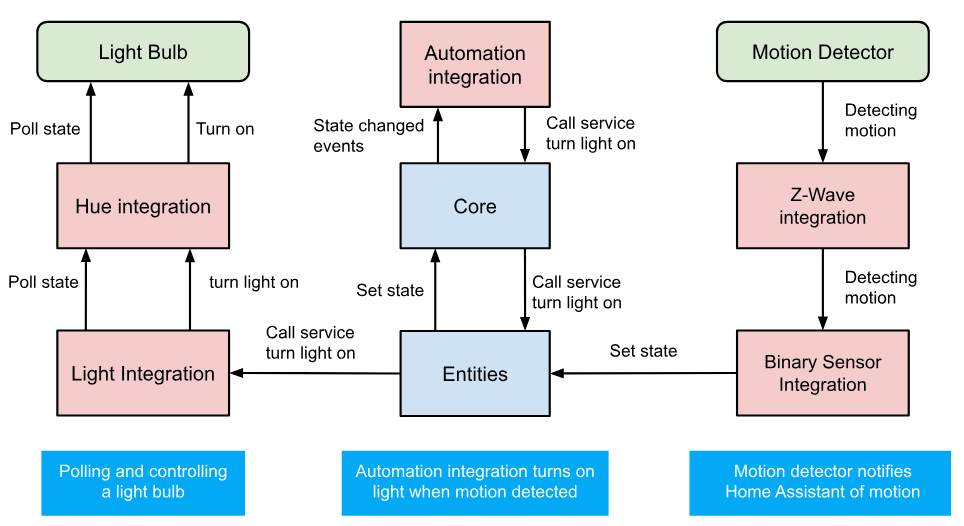
\includegraphics[width=\linewidth]{images/HA_integration_architechture.png}
    \caption{Integrationsarchitektur und Datenfluss zwischen externen Geräten, Core und Plattformen}
    \label{fig:integration-architecture}
\end{figure}

Wie in Abbildung~\ref{fig:integration-architecture} dargestellt, besteht eine vollständige Integration aus mehreren Bausteinen, die über sogenannte \texttt{Config Entries} initialisiert werden. Diese Konfigurationseinträge ermöglichen es, externe Geräte oder Dienste in Home Assistant einzubinden. 

Die Integration registriert ihre Entitäten über die \texttt{Entity Platform}, welche wiederum mit dem Core-Dienst kommuniziert. Dabei können die Entitäten regelmäßig abgefragt (Polling) oder bei Zustandsänderungen direkt aktualisiert werden. Über Registries wie die \texttt{Device Registry} und \texttt{Entity Registry} werden die Geräte und Entitäten systemweit verwaltet und eindeutig identifiziert.

Integrationen kommunizieren mit dem Core über:

\begin{itemize}
    \item den \textbf{Event Bus}, um auf Systemereignisse zu reagieren oder eigene Ereignisse auszulösen,\\
    \item das \textbf{Service Registry}, um eigene Aktionen (z.\,B. \texttt{light.turn\_on}) anzubieten,\\
    \item die \textbf{State Machine}, um Zustände von Entitäten zu lesen oder zu aktualisieren.
\end{itemize}

Die modulare Struktur und die lose Kopplung über Events und Services machen Home Assistant zu einer besonders flexiblen und erweiterbaren Plattform.

\subsubsection{Integrationstypen}

Home Assistant unterscheidet vier Typen von Integrationen:

\begin{itemize}
    \item \textbf{IoT-Domänen definieren:} Diese Integrationstypen wie \texttt{light} oder \texttt{switch} definieren, welche Datenformate und Steueraktionen für Geräte verfügbar sind.\\
    \item \textbf{Externe Geräte und Dienste anbinden:} Beispiele sind \texttt{Philips Hue} oder \texttt{MQTT}, die fremde Systeme integrieren.\\
    \item \textbf{Virtuelle/abgeleitete Daten:} Integrationen wie \texttt{template} oder \texttt{input\_boolean} erzeugen virtuelle Entitäten.\\
    \item \textbf{Automatisierung:} Integrationen wie \texttt{automation} oder \texttt{script} dienen zur Ablaufsteuerung.
\end{itemize}



\subsubsection{Struktur einer Custom Integration}

Eine benutzerdefinierte Integration liegt im Verzeichnis \\
\texttt{<config\_directory>/custom\_components/<name>} und besteht mindestens aus folgenden Dateien:

\begin{itemize}
    \item \texttt{manifest.json} – Enthält Metadaten wie Name, Domain, Abhängigkeiten, Version (bei Custom Integrationen zwingend erforderlich).\\
    \item \texttt{\_\_init\_\_.py} – Initialisiert die Integration und definiert z.\,B. die Setup-Funktion.\\
    \item Optional: \texttt{sensor.py}, \texttt{switch.py} etc. – Definieren die jeweiligen Plattformen (Entitätstypen).\\
    \item Optional: \texttt{config\_flow.py} – Definiert die Benutzeroberfläche für den Konfigurationsablauf.\\
    \item Optional: \texttt{translations}, \texttt{diagnostics}, \texttt{tests}.
\end{itemize}

\textbf{Home Assistant sucht nach Integrationen an zwei Stellen:}

\begin{enumerate}
    \item \texttt{<config\_directory>/custom\_components/<domain>} – für benutzerdefinierte (Custom) Integrationen.\\
    \item \texttt{homeassistant/components/<domain>} – für eingebaute (Core) Integrationen.
\end{enumerate}

Wird in der Konfiguration (z.\,B. \texttt{mobile\_app:}) eine Domain referenziert oder ist eine Integration eine Abhängigkeit einer anderen, versucht Home Assistant, die passende Integration automatisch zu laden. 

Ein besonderes Merkmal: Es ist möglich, eine eingebaute (Core) Integration zu überschreiben, indem man im Ordner \texttt{custom\_components} eine gleichnamige Integration bereitstellt. In diesem Fall ist im \texttt{manifest.json} zwingend ein \texttt{version}-Feld anzugeben. Überschriebene Core-Integrationen werden in der Benutzeroberfläche durch ein spezielles Symbol in der rechten oberen Ecke der Integrationskachel kenntlich gemacht.


\subsubsection{Config Flow}

Die Konfiguration erfolgt dynamisch über einen Konfigurationsdialog in der Weboberfläche von Home Assistant. Dieser Ablauf wird in der Datei \texttt{config\_flow.py} innerhalb des Integrationsverzeichnisses definiert. Dort wird eine eigene Klasse erstellt, die von \texttt{homeassistant.config\_entries.ConfigFlow} erbt. Der zugehörige Domain-Key muss beim Vererben übergeben werden, um die Konfiguration eindeutig der Integration zuordnen zu können.

Home Assistant nutzt hierbei das sogenannte \textit{Data Flow Entry Framework}, das die Interaktion mit dem Benutzer, die Validierung und Speicherung der Konfigurationsdaten übernimmt. Nach erfolgreicher Konfiguration werden die eingegebenen Werte in einem \texttt{ConfigEntry} gespeichert und automatisch im System registriert. Diese Konfigurationseinträge bilden die Grundlage für die Initialisierung und Wiederherstellung der Integration bei einem Neustart von Home Assistant.

Die Verwendung von \texttt{config\_flow.py} bietet den Vorteil, dass keine manuelle Bearbeitung der \texttt{configuration.yaml}-Datei notwendig ist und der Benutzer durch einen geführten Dialog zur Integration geführt wird.


\subsection{Home Assistant Entitäten}

Entitäten sind die kleinsten Funktionseinheiten in Home Assistant. Sie stehen für messbare Zustände oder steuerbare Funktionen – z.\,B. ein Sensorwert, ein Schalter oder eine Zeitschaltuhr. Jede Entität gehört zu einer Domain (z.\,B. \texttt{sensor}, \texttt{light}, \texttt{switch}) und wird über eine eindeutige Kennung wie \texttt{sensor.wohnzimmer\_temperatur} identifiziert.

Entitäten werden durch Integrationen erzeugt, die Geräte oder Dienste einbinden. Die jeweiligen Datenpunkte eines Geräts oder Dienstes werden über Entitäten in Home Assistant abgebildet. Standardisierte Domains wie \texttt{light} oder \texttt{switch} bieten vordefinierte Aktionen wie \texttt{turn\_on}, während Integrationen auch eigene nicht-standardisierte Services registrieren können – z.\,B. \texttt{hue.activate\_scene}.

Aus Entwicklersicht verbirgt eine Entität die internen Details der Plattform. Integratoren müssen lediglich von einer Basisklasse wie \texttt{SensorEntity} oder \texttt{SwitchEntity} erben und die relevanten Eigenschaften und Methoden für das jeweilige Gerät implementieren. Die Anbindung erfolgt dabei entweder über einen Konfigurationseintrag (\texttt{ConfigEntry}) oder in Legacy-Fällen über die \texttt{configuration.yaml}.

Die zentrale Architektur sieht vor, dass:

\begin{itemize}
    \item die Geräteintegration (z.\,B. \texttt{hue}) das Gerät über die bereitgestellte Konfiguration verbindet,\\
    \item anschließend die Entitäten für die jeweilige Domain (z.\,B. \texttt{light}) eingerichtet werden,\\
    \item die \texttt{EntityPlatform} die Verwaltung und das Polling der Entitäten übernimmt,\\
    \item die \texttt{EntityComponent} die Services verteilt und Discovery-Informationen weiterleitet.
\end{itemize}

Integrationen können auch eigene Dienste registrieren, die für alle von ihnen erzeugten Entitäten gelten. Diese Dienste werden unter der Domain der Geräteintegration veröffentlicht und wirken auf alle entsprechenden Entitäten (z.\,B. alle Hue-Leuchten).


\subsubsection{Registrierung und Verwaltung}

\texttt{EntityPlatform} übernimmt die Verwaltung aller Entitäten einer Plattform und ermöglicht deren dynamisches Hinzufügen. \texttt{EntityComponent} gruppiert Entitäten pro Domain und verteilt Service-Aufrufe. Alle registrierten Entitäten werden in der \texttt{Entity Registry} gespeichert, was auch nach einem Neustart eine Wiederherstellung der Konfiguration ermöglicht.

\subsubsection{Geräte und Entitäten registrieren}

\begin{figure}[H]
    \centering
    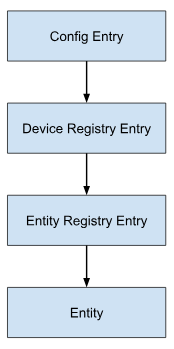
\includegraphics[width=0.35\linewidth]{images/entity_heirarchy.png}
    \caption{Registrierung von Geräten und Entitäten über ein Konfigurationseintrag}
    \label{fig:entity-reg-hierarchy}
\end{figure}

Ein \texttt{ConfigEntry} erzeugt automatisch Einträge im \texttt{Device Registry} und \texttt{Entity Registry} (siehe Abbildung~\ref{fig:entity-reg-hierarchy}). Damit sind Entitäten systemweit auffindbar, eindeutig zuordenbar und auch nach Neustarts persistent verfügbar.

\subsubsection{Interaktion mit dem Home Assistant Core}

\begin{figure}[H]
    \centering
    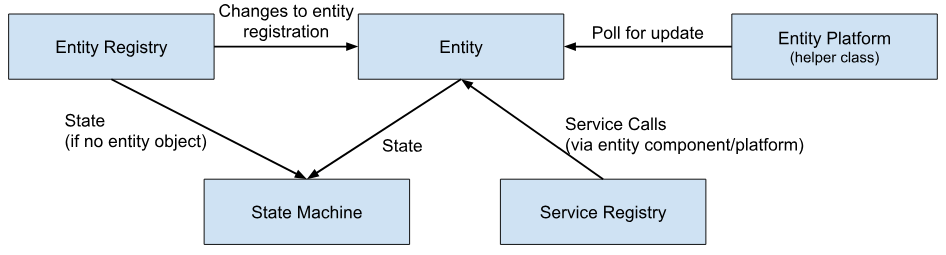
\includegraphics[width=\linewidth]{images/simp_entity.png}
    \caption{Zusammenspiel zwischen Entität, Event Bus, State Machine und Service Registry}
    \label{fig:entity-core-interaction}
\end{figure}

Wie in Abbildung~\ref{fig:entity-core-interaction} zu sehen, interagiert jede Entität mit den zentralen Subsystemen:

\begin{itemize}
    \item \textbf{State Machine:} Speichert den aktuellen Zustand jeder Entität (z.\,B. \texttt{on}, \texttt{23.5} etc.)\\
    \item \textbf{Event Bus:} Versendet bei jeder Zustandsänderung ein \texttt{state\_changed}-Event.\\
    \item \textbf{Service Registry:} Nimmt Service-Aufrufe wie \texttt{turn\_on}, \texttt{reset} oder benutzerdefinierte Aktionen entgegen.
\end{itemize}

\begin{figure}[H]
    \centering
    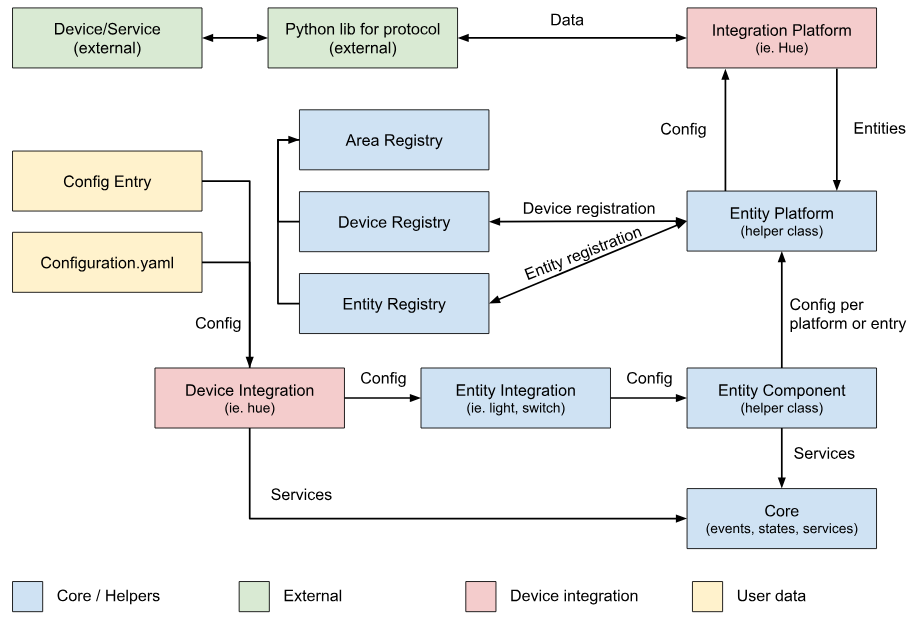
\includegraphics[width=\linewidth]{images/Entity_interaction_Home_assistant.png}
    \caption{Detailliertes Zusammenspiel zwischen Integration, Entitätsplattform und Core}
    \label{fig:entity-detailed}
\end{figure}

Abbildung~\ref{fig:entity-detailed} illustriert die vollständige Interaktion: Die \texttt{Integration Platform} – etwa \texttt{hue.light} – nutzt die Konfiguration, um externe Geräte abzufragen und daraus Entitäten zu erzeugen. Diese Entitäten werden über \texttt{Entity Platform} hinzugefügt und mit der \texttt{Entity Registry} sowie \texttt{Device Registry} verknüpft. Der \texttt{Entity Component} verteilt schließlich die Service-Aufrufe und sorgt für eine einheitliche Behandlung durch den Core.


\subsubsection{Polling vs. Push}

Standardmäßig ruft Home Assistant regelmäßig den aktuellen Zustand per Polling über \texttt{update()} oder \texttt{async\_update()} ab. Alternativ kann eine Entität bei Änderung über \\ \texttt{schedule\_update\_ha\_state()} ihre neue Information pushen.

\subsubsection{Zusammenfassung}

Die Architektur von Integrationen und Entitäten erlaubt eine modulare, lose gekoppelte und erweiterbare Steuerung beliebiger Geräte und Dienste innerhalb von Home Assistant. Diese Struktur wird insbesondere bei der Implementierung eigener Integrationen wie im KaVo-Projekt genutzt, um neue medizinische Geräte lokal und dynamisch steuerbar zu machen.

\subsection{Geräteautomatisierung in Home Assistant}

Home Assistant bietet eine leistungsstarke und dennoch benutzerfreundliche Möglichkeit zur Erstellung von Automationen, mit denen Geräte anhand von Ereignissen, Zuständen und Zeitbedingungen gesteuert werden können. Diese Automationen bestehen typischerweise aus drei zentralen Bestandteilen:

\subsubsection{Trigger (Auslöser)}
Ein Trigger definiert, wann eine Automation ausgelöst werden soll. In unserem Fall wird die Automation aktiviert, wenn sich der Zustand der Entität \texttt{Hygiene Plan Phase} ändert – zum Beispiel auf \enquote{Abends Hygiene process completed}.

\begin{figure}[H]
    \centering
    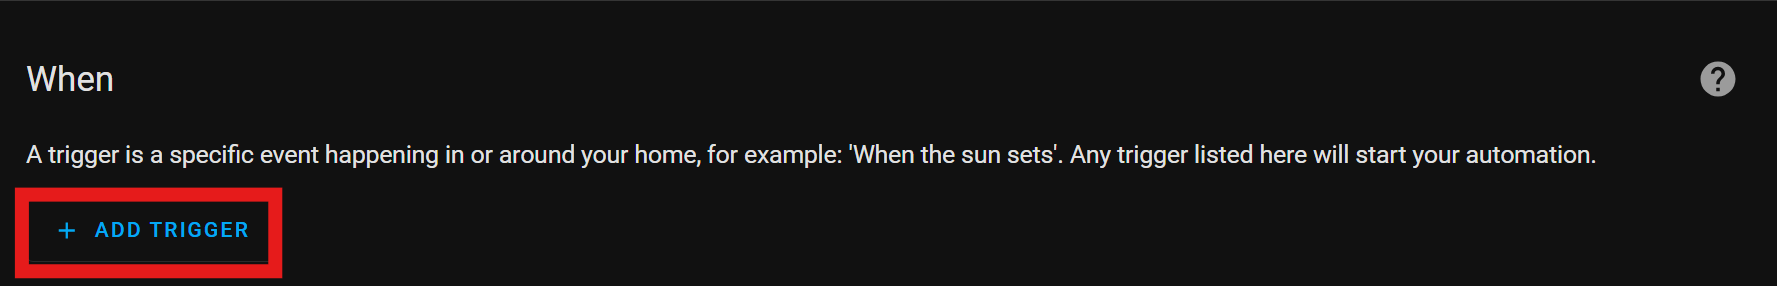
\includegraphics[width=\linewidth]{images/auto_addtrig1.png}
    \caption{Startpunkt – Einen Trigger hinzufügen}
\end{figure}

\begin{figure}[H]
    \centering
    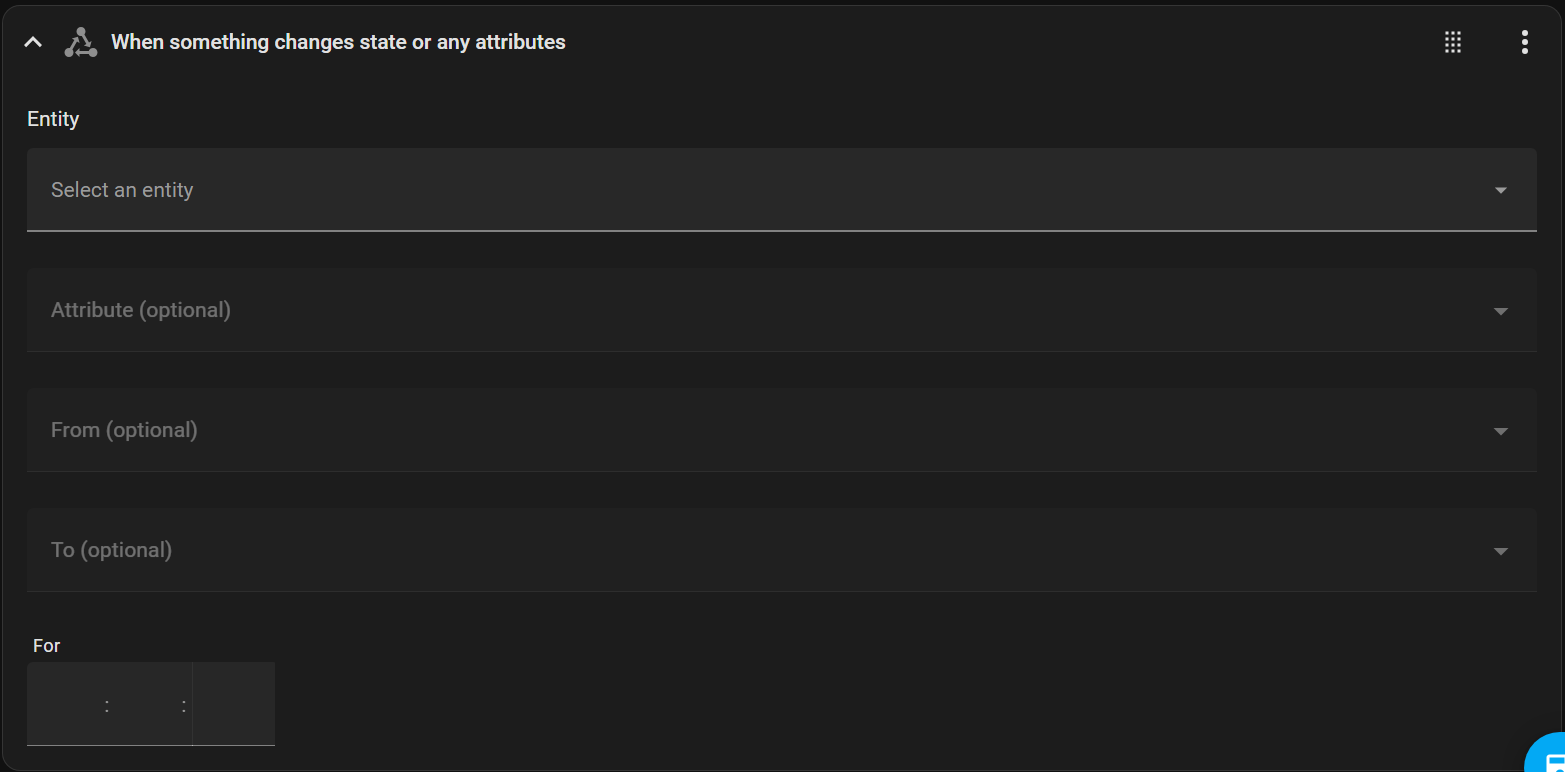
\includegraphics[width=\linewidth]{images/auto_trig1.png}
    \caption{Erstellung eines Triggers}
\end{figure}

\begin{figure}[H]
    \centering
    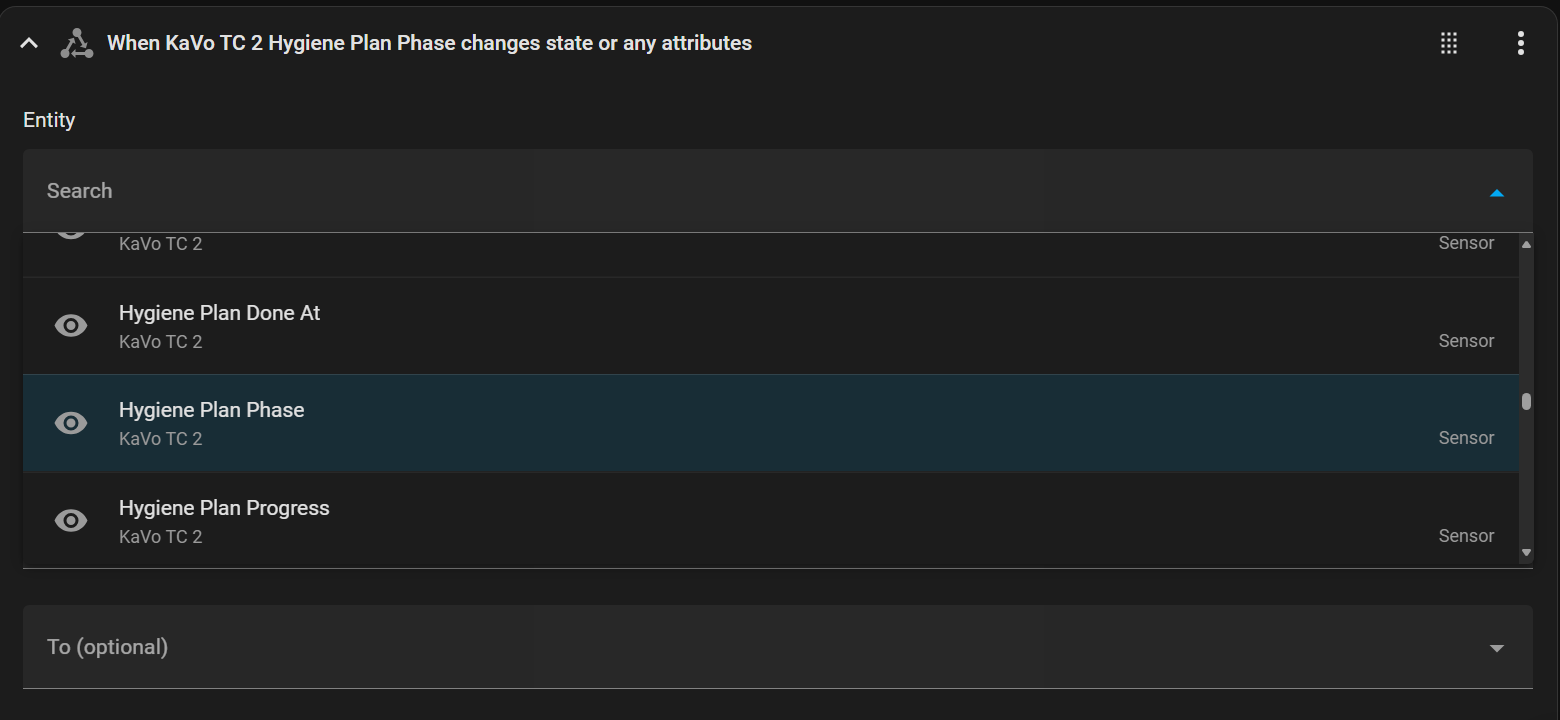
\includegraphics[width=\linewidth]{images/auto_trig2.png}
    \caption{Auswahl der Entität für den Trigger}
\end{figure}

\begin{figure}[H]
    \centering
    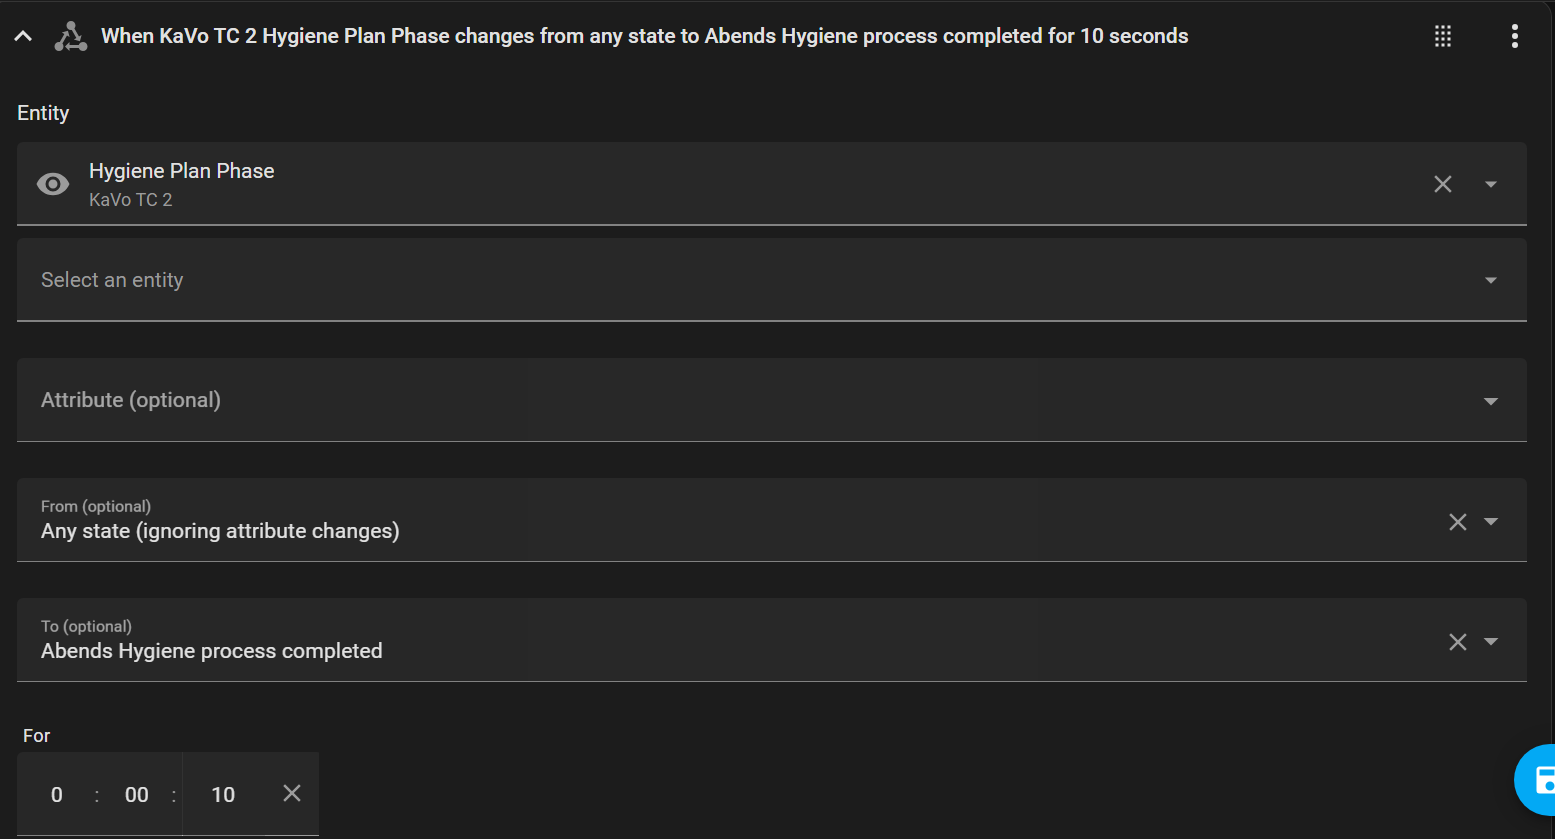
\includegraphics[width=\linewidth]{images/auto_trig3.png}
    \caption{Feineinstellung der Auslösebedingungen}
\end{figure}


\subsubsection{Conditions (Bedingungen)}
Bedingungen sind optional und definieren, ob eine ausgelöste Automation wirklich ausgeführt werden soll. In unseren Automationen wurden keine zusätzlichen Bedingungen gesetzt, da allein der Zustand des Hygieneplans zur Entscheidung genügt.

\subsubsection{Actions (Aktionen)}
Die Aktion legt fest, was passieren soll, wenn die Automation ausgelöst wird. In unserem Fall wird der \texttt{Shelly Pro 1PM} ausgeschaltet.

\begin{figure}[H]
    \centering
    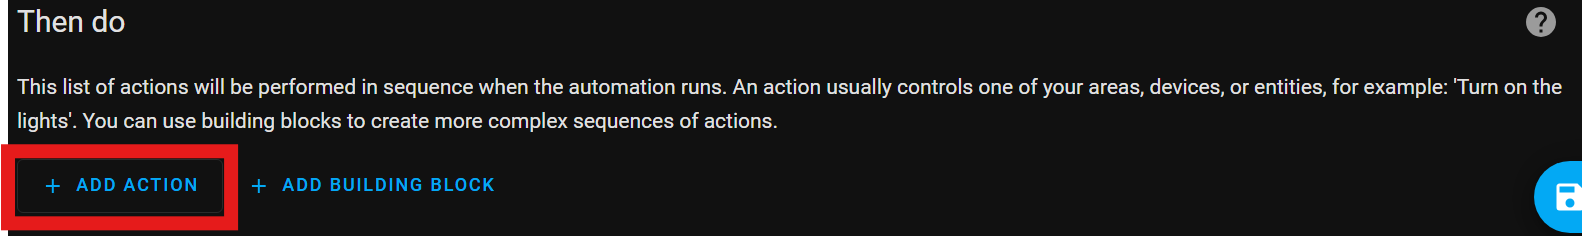
\includegraphics[width=0.8\linewidth]{images/auto_addaction.png}
    \caption{Button zum Hinzufügen einer Aktion}
\end{figure}

\begin{figure}[H]
    \centering
    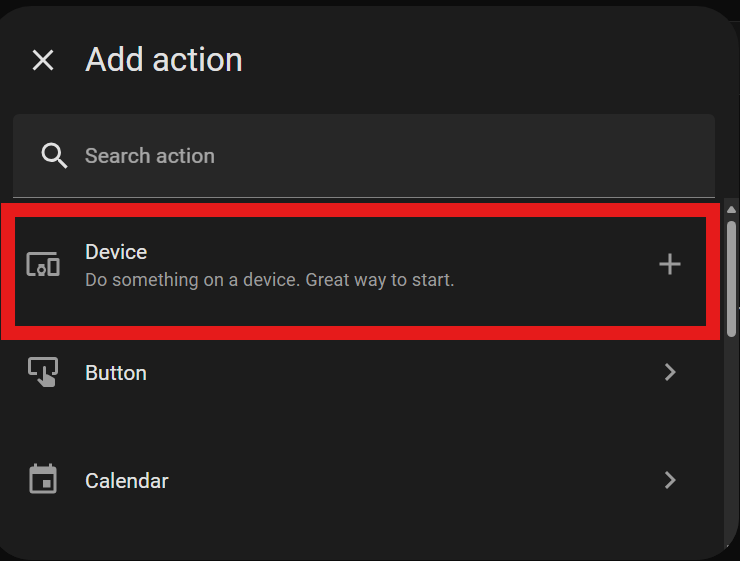
\includegraphics[width=\linewidth]{images/auto_action2.png}
    \caption{Auswahl verschiedener Aktionsarten: Gerät, Szene, Dienst, Kalender usw.}
\end{figure}

\begin{figure}[H]
    \centering
    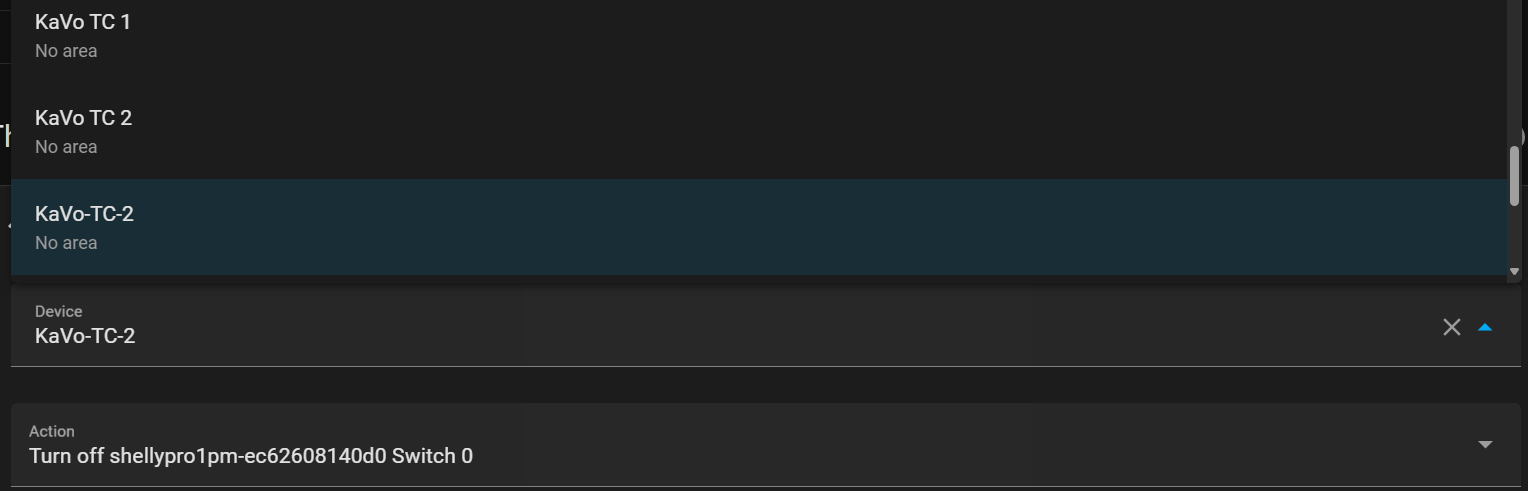
\includegraphics[width=\linewidth]{images/auto_action3.png}
    \caption{Auswahl des Geräts, auf das die Aktion angewendet werden soll}
\end{figure}

\begin{figure}[H]
    \centering
    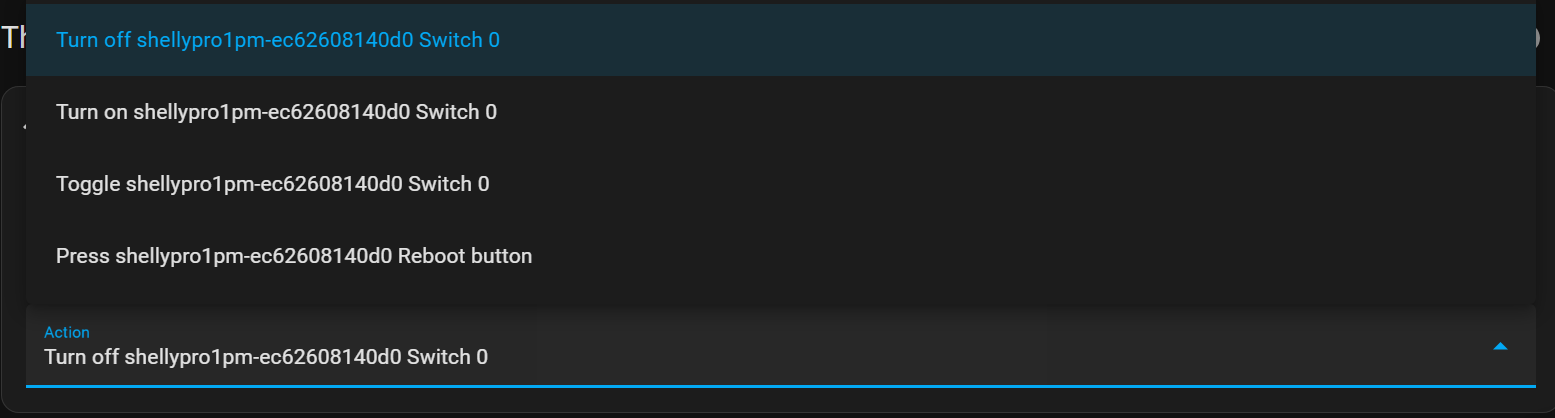
\includegraphics[width=\linewidth]{images/auto_trigaction4.png}
    \caption{Liste verfügbarer Aktionen für das gewählte Gerät}
\end{figure}

\subsubsection{Automation erstellen}
Der gesamte Automatisierungsprozess kann vollständig über die grafische Benutzeroberfläche von Home Assistant durchgeführt werden, was eine einfache Konfiguration durch nicht-technische Stakeholder ermöglicht.

Zunächst navigiert man in der Seitenleiste zu \texttt{Automations \& Scenes}, wie in Abbildung~\ref{fig:auto_find} dargestellt. Anschließend klickt man auf \texttt{Create Automation} (Abbildung~\ref{fig:auto_create1}) und wählt \texttt{Create new automation}, um mit einer leeren Automation zu beginnen (Abbildung~\ref{fig:auto_create2}).

\begin{figure}[H]
    \centering
    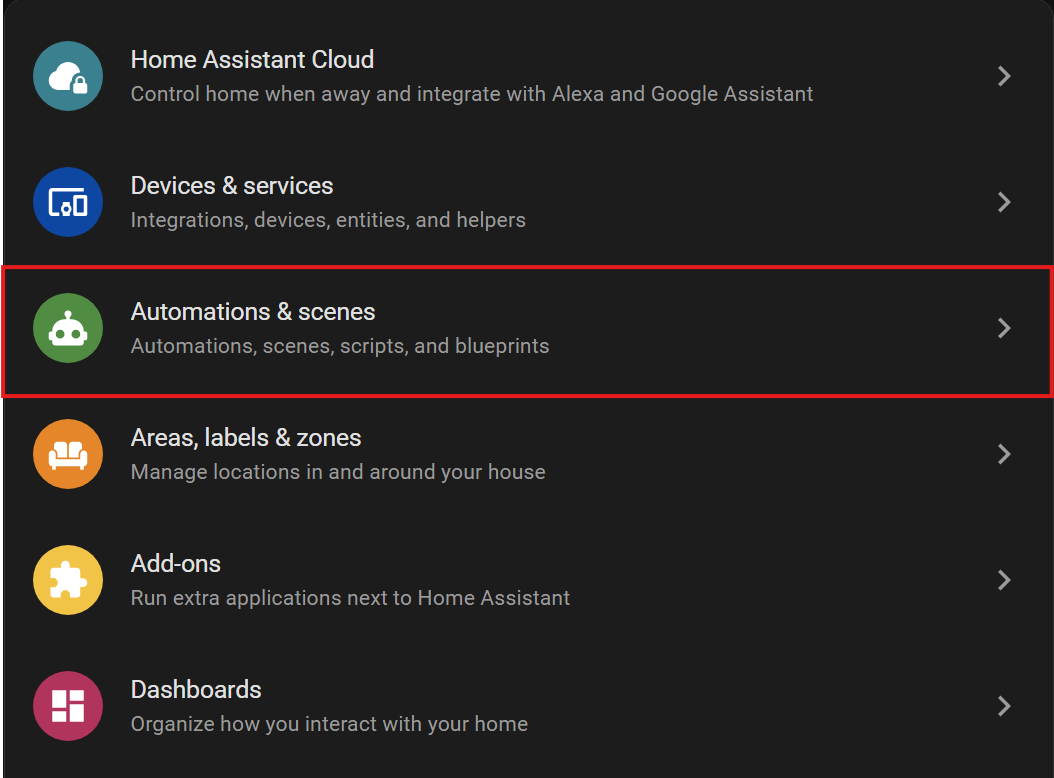
\includegraphics[width=0.7\linewidth]{images/auto_find.png}
    \caption{Navigieren zum Bereich Automatisierungen}
    \label{fig:auto_find}
\end{figure}

\begin{figure}[H]
    \centering
    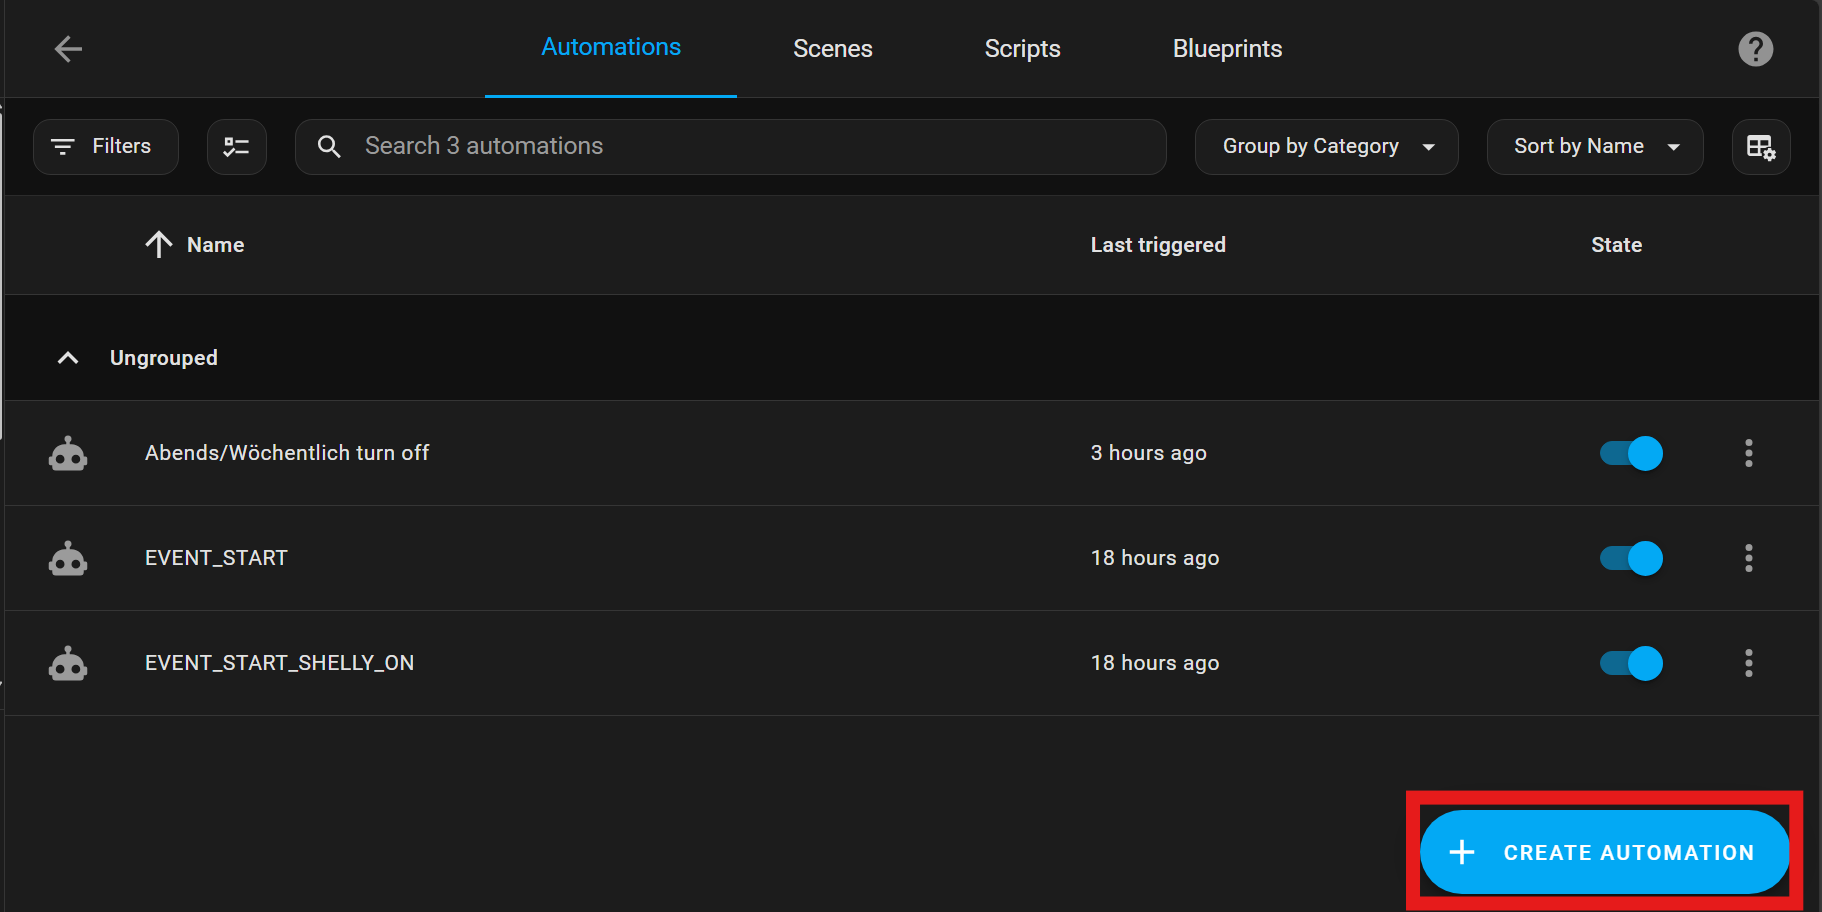
\includegraphics[width=0.7\linewidth]{images/auto_create1.png}
    \caption{Neue Automation erstellen}
    \label{fig:auto_create1}
\end{figure}

\begin{figure}[H]
    \centering
    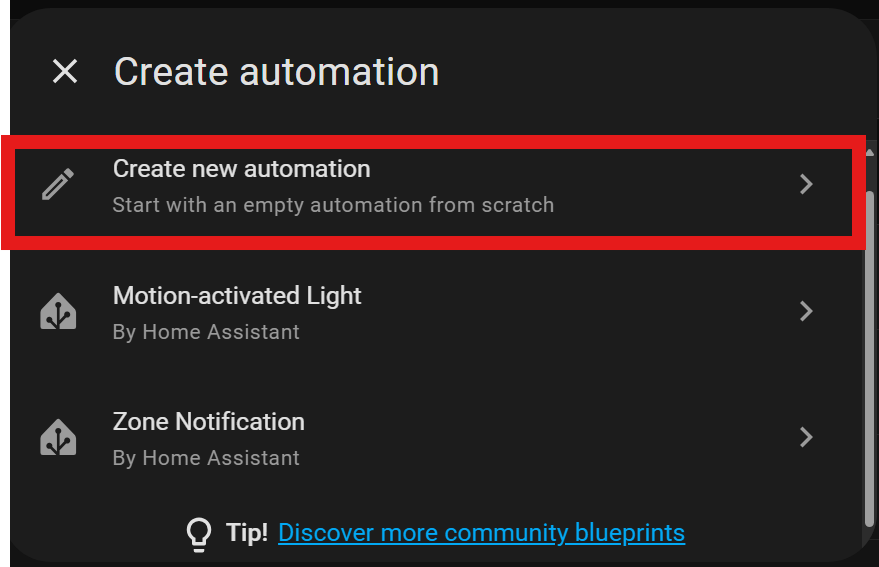
\includegraphics[width=0.7\linewidth]{images/auto_create2.png}
    \caption{Leere Automation starten}
    \label{fig:auto_create2}
\end{figure}

Die Erstellung erfolgt in drei Schritten:
\begin{itemize}
    \item \textbf{Trigger hinzufügen}: Definiert, wann die Automation ausgelöst werden soll (siehe Abbildung~\ref{fig:auto_addtrig1}).\\
    \item \textbf{Aktion definieren}: Legt fest, was bei Auslösung geschehen soll (siehe Abbildung~\ref{fig:auto_addaction}).\\
    \item \textbf{Automation speichern}: Abschluss der Konfiguration (siehe Abbildung~\ref{fig:auto_save}).
\end{itemize}

\begin{figure}[H]
    \centering
    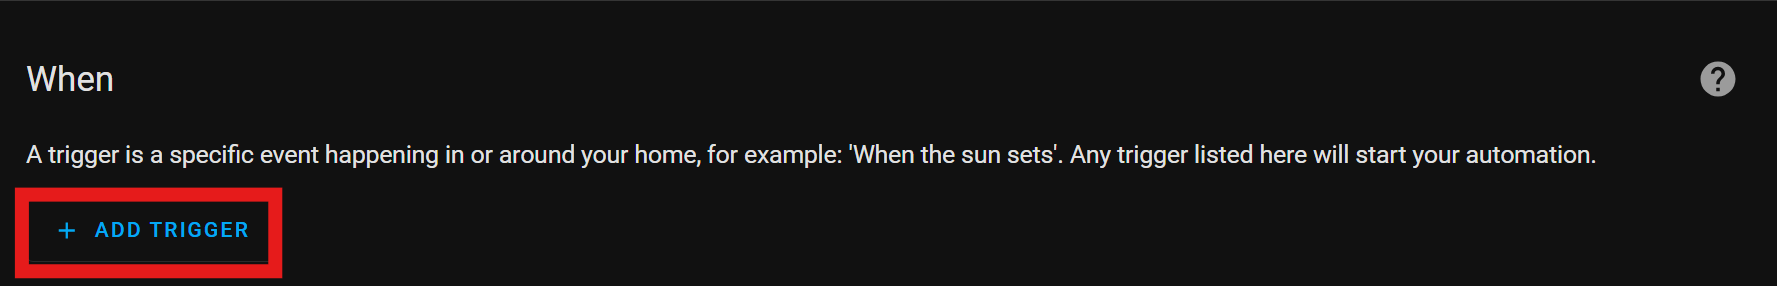
\includegraphics[width=0.7\linewidth]{images/auto_addtrig1.png}
    \caption{Trigger hinzufügen}
    \label{fig:auto_addtrig1}
\end{figure}

\begin{figure}[H]
    \centering
    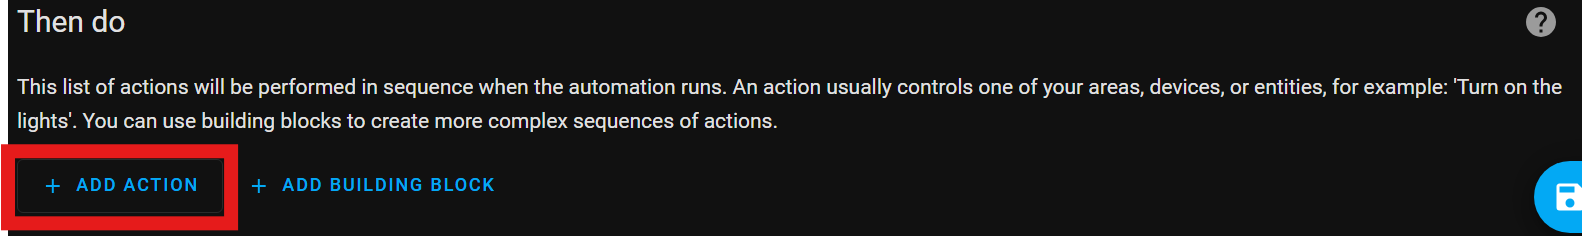
\includegraphics[width=0.7\linewidth]{images/auto_addaction.png}
    \caption{Aktion definieren}
    \label{fig:auto_addaction}
\end{figure}

\begin{figure}[H]
    \centering
    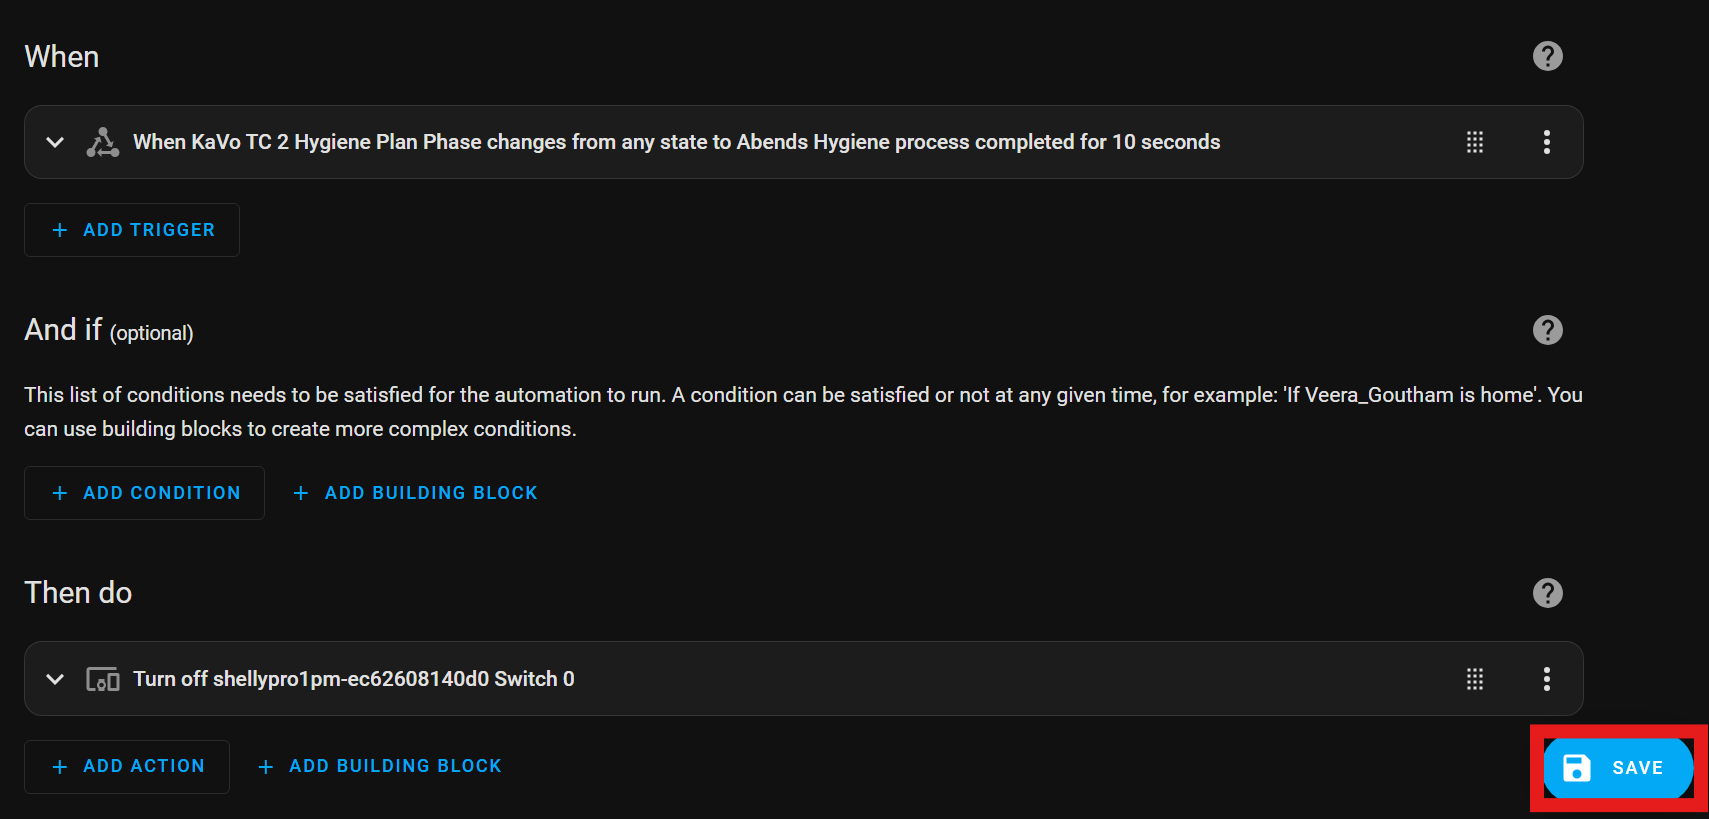
\includegraphics[width=0.7\linewidth]{images/auto_save.png}
    \caption{Automation speichern}
    \label{fig:auto_save}
\end{figure}


\subsubsection{Modus: \texttt{parallel}}

In Home Assistant bestimmt der sogenannte \textbf{Modus} (\textit{mode}), wie eine Automation auf mehrere gleichzeitige Auslösungen reagiert. Wenn z.\,B. ein Trigger mehrfach in kurzer Zeit ausgelöst wird – etwa durch mehrere Geräte oder Benutzerinteraktionen – legt der Modus fest, wie damit umgegangen wird. Zur Auswahl stehen folgende Modi:
\begin{itemize}
  \item \texttt{single}: Führt die Automation nur einmal aus. Weitere Auslösungen während der Laufzeit werden ignoriert.\\
  \item \texttt{restart}: Bricht die laufende Automation ab und startet sie neu.\\
  \item \texttt{queued}: Wartet mit der neuen Ausführung, bis die aktuelle abgeschlossen ist.\\
  \item \texttt{parallel}: Führt die Automation mehrfach gleichzeitig aus. Jede Auslösung wird unabhängig behandelt.
\end{itemize}

\medskip
\textbf{Warum wurde \texttt{parallel} gewählt?} \\
In diesem Projekt kommunizieren mehrere KaVo-Dentaleinheiten unabhängig voneinander mit Home Assistant. Jede Einheit übermittelt ihren Hygienezeitplan separat per WebSocket. Wenn mehrere Einheiten nahezu gleichzeitig ein Hygieneprogramm starten, muss Home Assistant in der Lage sein, mehrere Automationen gleichzeitig zu verarbeiten. Der \texttt{parallel}-Modus stellt sicher, dass jede dieser Auslösungen unabhängig behandelt wird und keine Aktionen verloren gehen oder blockiert werden.

\medskip
\textbf{Einstellen des Modus in der Benutzeroberfläche} \\
Nachdem eine Automation gespeichert wurde, kann der Modus wie folgt geändert werden:
\begin{enumerate}
  \item Die Automation in der Übersicht auswählen.
  \item Über das Kontextmenü oben rechts (drei Punkte) den Punkt \enquote{Change mode} wählen.
  \item Im Dialog \enquote{Change mode} den gewünschten Modus – hier \texttt{parallel} – auswählen und auf \enquote{Change mode} klicken.
\end{enumerate}

\begin{figure}[H]
    \centering
    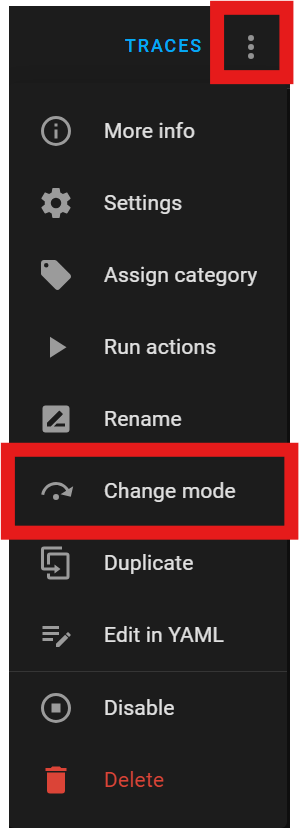
\includegraphics[width=0.45\linewidth]{images/changemode_1.png}
    \caption{Kontextmenü zum Ändern des Automationsmodus}
\end{figure}

\begin{figure}[H]
    \centering
    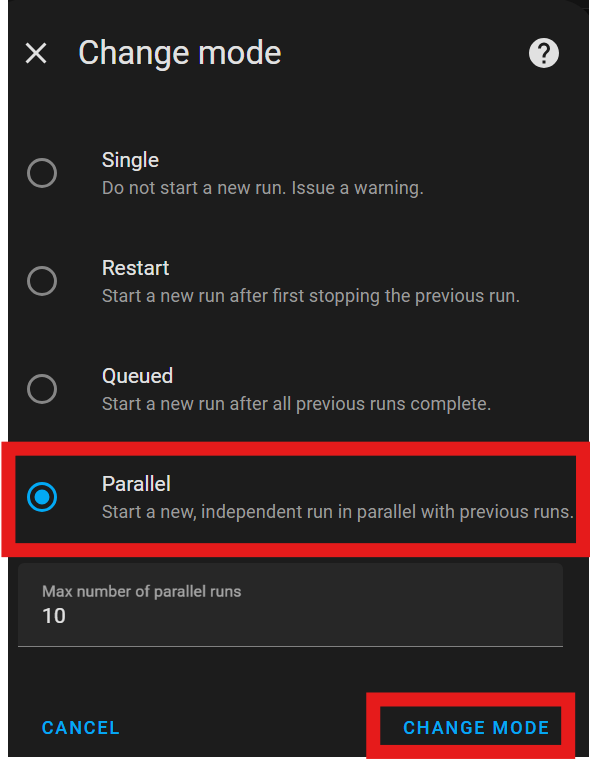
\includegraphics[width=0.55\linewidth]{images/changemode2.png}
    \caption{Auswahl des Modus \texttt{Parallel} zur gleichzeitigen Ausführung}
\end{figure}



\subsection{KaVo Integration}

Im Rahmen dieser Arbeit wurde eine benutzerdefinierte Home-Assistant-Integration mit dem Namen \texttt{KaVo\_Integration} entwickelt, um eine KaVo-Dentaleinheit lokal in ein Smart-Home-System zu integrieren. Ziel der Integration ist es, Daten aus der Dentaleinheit in Echtzeit zu visualisieren, Automatisierungen zu ermöglichen (z.\,B. Hygieneprogramme) – und das vollständig ohne Cloud-Anbindung.

Die Integration wurde gemäß den Home-Assistant-Richtlinien strukturiert und verwendet moderne Konzepte wie \texttt{Config Flow}, dynamische Entitätenerstellung und eine WebSocket-Kommunikation. 

Zum Betrieb von Home Assistant wurde ein \textbf{Raspberry Pi 400} verwendet, auf dem das \textbf{Home Assistant OS} direkt installiert wurde. Damit steht eine autarke, energieeffiziente und leicht zugängliche Smart-Home-Plattform zur Verfügung. Die Benutzeroberfläche von Home Assistant ist über den Webbrowser unter der lokalen IP-Adresse des Geräts erreichbar (z.\,B. \texttt{http://homeassistant.local:8123} oder per IP-Adresse wie \texttt{http://192.168.1.x:8123}).
\newpage
\textbf{Die Projektstruktur ist wie folgt aufgebaut:}

\begin{figure}[H]
\centering
\begin{minipage}{0.75\textwidth}
\begin{itemize}
  \item \textbf{/custom\_components/KaVo\_Integration/}
  \begin{itemize}
    \item \texttt{\_\_init\_\_.py}     (Initialisierung der Integration)
    \item \texttt{config\_flow.py}     (Konfigurationsdialog über UI)
    \item \texttt{manifest.json}       (Metadaten zur Integration)
    \item \texttt{const.py}            (Globale Konstanten (z.\,B. \texttt{DOMAIN}, Event-Namen))
    \item \texttt{websocket\_client.py}  (Asynchroner WebSocket-Client)
    \item \texttt{sensor.py}             (Erstellung dynamischer Sensor-Entitäten)
    \item \texttt{binary\_sensor.py}     (Verbindungssensor zur Statusanzeige des Servers)
    \item \texttt{calendar.py}           (Abbildung des Hygieneplans als Kalenderentität)
  \end{itemize}
\end{itemize}
\end{minipage}
\caption{Dateistruktur der Custom-Integration \texttt{KaVo\_Integration} in Home Assistant}
\label{fig:kavo-integration-structure}
\end{figure}
\vspace{0.5cm}


Die Integration erlaubt das gleichzeitige Hinzufügen mehrerer Dentaleinheiten im selben Netzwerk. Diese werden über mDNS (Zeroconf) automatisch entdeckt, wodurch der Einrichtungsprozess für den Endnutzer erheblich vereinfacht wird. Weitere Details zu den einzelnen Komponenten und deren Funktionsweise folgen in den nachfolgenden Abschnitten.

\subsubsection{manifest.json}

Die Datei \texttt{manifest.json} dient als zentrale Metadatendatei für jede Home Assistant Integration. Sie beschreibt grundlegende Eigenschaften wie Domain, Name, Version, unterstützte Plattformen und Konfigurationsmethoden. Ohne diese Datei kann eine benutzerdefinierte Integration nicht erkannt oder geladen werden.

\textbf{Erklärung der wichtigsten Felder:}

\begin{itemize}
    \item \texttt{domain}: Eindeutiger Bezeichner der Integration. Wird im Pfad und der Systemstruktur verwendet.\\
    \item \texttt{name}: Anzeigename in der Benutzeroberfläche.\\
    \item \texttt{version}: Notwendig bei Custom Integrations, vor allem für Updates via HACS.\\
    \item \texttt{config\_flow}: Aktiviert die Benutzerführung zur Konfiguration über die Oberfläche.\\
    \item \texttt{zeroconf}: Definiert mDNS-Dienste, über die die Integration automatisch erkannt werden kann.\\
    \item \texttt{platforms}: Verweist auf unterstützte Plattformdateien wie \texttt{sensor.py}, \texttt{calendar.py} etc.
\end{itemize}

\vspace{1em}
\textbf{Zusätzliche Hinweise:}

\begin{itemize}
    \item Benutzerdefinierte Integrationen werden unter \texttt{config/custom\_components/<domain>} gespeichert.\\
    \item Durch das Definieren von \texttt{zeroconf} kann Home Assistant Geräte automatisch erkennen und die Integration vorschlagen.\\
    \item Beim Überschreiben einer Core-Integration muss \texttt{version} angegeben sein.
\end{itemize}

\vspace{1em}
\textbf{Fazit}

Die Datei \texttt{manifest.json} ist für die korrekte Registrierung und Initialisierung einer Integration essenziell. Sie erlaubt es Home Assistant, die Integration systemweit sichtbar zu machen, ihre Konfiguration zu ermöglichen und die dazugehörigen Plattformdateien korrekt zu laden.

\subsubsection{config\_flow.py}

Diese Datei steuert den vollständigen Konfigurationsablauf der Integration in der Home Assistant-Benutzeroberfläche. Sie ermöglicht sowohl die automatische Erkennung (via mDNS/Zeroconf) als auch die manuelle Einrichtung einer KaVo-Dentaleinheit.

\vspace{0.5cm}

\textbf{Zweck von \texttt{config\_flow.py}:}

Die Datei \texttt{config\_flow.py} enthält die zentrale Klasse \texttt{TestChairConfigFlow}, die von \texttt{ConfigFlow} erbt und das Verhalten bei der Einrichtung definiert:

\begin{itemize}
\item Unterstützung von \textbf{Zeroconf-Erkennung} (mDNS) über \texttt{async\_step\_zeroconf}.\\
\item Manuelle Einrichtung über die UI mit \texttt{async\_step\_user}.\\
\item Erzeugung eines \texttt{ConfigEntry}-Objekts mit \texttt{async\_create\_entry}, das später von \texttt{async\_setup\_entry} (in \texttt{\_\_init\_\_.py}) verwendet wird.\\
\item In diesem Schritt werden die IP-Adresse der Dentaleinheit sowie der Port gespeichert, der aus dem über mDNS empfangenen Service-Datensatz stammt. Diese Informationen sind notwendig, um später in \texttt{websocket\_client.py} eine Verbindung zum WebSocket-Server der Dentaleinheit herstellen zu können.

\end{itemize}

\vspace{0.5cm}

\textbf{Wichtige Imports und ihre Funktion:}

\begin{tabular}{|p{5.5cm}|p{8.5cm}|}
\hline
\textbf{Modul} & \textbf{Zweck} \\
\hline
\texttt{config\_entries}, \texttt{CONF\_HOST} & Home Assistant API für dynamische Konfiguration \\
\texttt{voluptuous} & Schema-Validierung für Benutzereingaben \\
\texttt{DOMAIN} & Konstante zur Identifizierung der Integration \\
\texttt{logging} & Ausgabe von Debug- und Fehlernachrichten \\
\hline
\end{tabular}

\vspace{0.5cm}

\textbf{Ablauf bei automatischer Erkennung via Zeroconf:}

\begin{itemize}
\item \texttt{async\_step\_zeroconf} wird aufgerufen, wenn Home Assistant ein Gerät über mDNS erkennt (weil \texttt{manifest.json} den Dienst \texttt{\_kavochair.\_tcp.local.} angibt).
\item Die Methode extrahiert \texttt{host}, \texttt{port}, \texttt{hostname}, \texttt{name}, \texttt{manufacturer}, \texttt{model}, \texttt{version}.
\item \texttt{self.async\_set\_unique\_id(name)} setzt eine eindeutige Geräte-ID.
\item Danach wird ein Bestätigungsdialog angezeigt: \texttt{async\_step\_zeroconf\_confirm}.
\item Wenn der Benutzer bestätigt, wird ein \texttt{ConfigEntry} erzeugt.
\end{itemize}

\vspace{0.5cm}

\textbf{Bestätigungsformular: \texttt{async\_step\_zeroconf\_confirm}}

\begin{itemize}
\item Zeigt ein einfaches Bestätigungsformular, um versehentliche Geräteerkennungen zu vermeiden.\\
\item Nach Bestätigung wird die Konfiguration gespeichert und das Gerät hinzugefügt.
\end{itemize}

\vspace{0.5cm}

\textbf{Manuelle Einrichtung: \texttt{async\_step\_user}}

\begin{itemize}
\item Ermöglicht die Eingabe von Host und Port durch den Benutzer.\\
\item Es wird überprüft, ob bereits eine Instanz mit dieser eindeutigen ID besteht.\\
\item Falls nicht, wird ebenfalls ein \texttt{ConfigEntry} erzeugt.\\
\end{itemize}

\vspace{0.5cm}

\textbf{Übergang zu \texttt{async\_setup\_entry}:}

Die in \texttt{config\_flow.py} gesammelten Konfigurationsdaten werden in einem \texttt{ConfigEntry} gespeichert. Dieses wird dann im Datei \texttt{\_\_init\_\_.py} von der Methode \texttt{async\_setup\_entry} verarbeitet. Hier werden:

\begin{itemize}
\item WebSocket-Client erstellt und mit dem Gerät verbunden.\\
\item Metadaten registriert (\texttt{device\_registry}).\\
\item Sensor-, Binary-Sensor- und Kalender-Plattformen initialisiert.
\end{itemize}

\vspace{0.5cm}

\textbf{Fazit:}

Die Klasse \texttt{TestChairConfigFlow} ermöglicht eine einfache und intuitive Integration neuer KaVo-Dentaleinheiten – entweder durch automatische Erkennung oder manuelle Eingabe. Die Struktur stellt sicher, dass Duplikate vermieden werden, alle Konfigurationsdaten persistent gespeichert sind und das Setup nahtlos in Home Assistant integriert ist.

\subsubsection{\_\_init\_\_.py}

Diese Datei dient als Einstiegspunkt für die Home Assistant-Integration. Sie wird automatisch geladen, wenn Home Assistant startet oder ein neues Konfigurationsobjekt (ConfigEntry) für die Integration angelegt wird.

\vspace{0.5cm}
\textbf{Zweck von \texttt{\_\_init\_\_.py}:}

\begin{itemize}
  \item Initialisierung beim Start von Home Assistant.\\
  \item Einrichtung bei neuer Gerätekonfiguration über UI oder Zeroconf.\\
  \item Starten eines asynchronen WebSocket-Clients.\\
  \item Registrierung des Geräts im Device Registry.\\
  \item Weiterleitung an Plattformdateien (\texttt{sensor.py}, \texttt{binary\_sensor.py}, \texttt{calendar.py}).\\
  \item Ressourcenfreigabe bei Gerätemigration oder Löschung.
\end{itemize}
\vspace{0.5cm}

\textbf{Wichtige Imports und ihre Funktion:}

\begin{tabular}{|p{5cm}|p{9cm}|}
\hline
\textbf{Modul} & \textbf{Zweck} \\
\hline
\texttt{logging} & Logging für Debug und Statusmeldungen \\
\texttt{.websocket\_client} & Interne WebSocket-Kommunikation zur Geräteeinheit \\
\texttt{device\_registry} & Zugriff auf das zentrale Geräteverzeichnis von Home Assistant \\
\texttt{config\_entries}, \texttt{core} & Bereitstellung der Setup-Schnittstellen \\
\texttt{.const.DOMAIN} & Eindeutige Domäne der Integration \\
\hline
\end{tabular}

\vspace{0.5cm}

\textbf{\texttt{async\_setup(hass, config)}:}

Diese Funktion wird beim Start von Home Assistant aufgerufen – unabhängig davon, ob bereits Geräte konfiguriert wurden. Sie gibt einfach \texttt{True} zurück.

\vspace{0.5cm}

\textbf{\texttt{async\_setup\_entry(hass, entry)}:}

Diese Methode ist zentral für das Setup eines konfigurierten Geräts und folgt folgendem Ablauf:

\begin{itemize}
  \item Auslesen der Verbindungsdaten: \texttt{host}, \texttt{port}, \texttt{hostname}, etc.\\
  \item Erstellen eines WebSocket-Clients und Speichern in \texttt{hass.data[DOMAIN][entry\_id]}.\\
  \item Aufbau einer gemeinsamen Speicherstruktur für Sensoren, Kalender, etc.\\
  \item Registrierung im \texttt{Device Registry} mit Hersteller-, Modell- und Versionsinformationen.\\
  \item Weiterleiten des Eintrags an Plattformdateien über \texttt{async\_forward\_entry\_setups}.\\
  \item Starten der WebSocket-Verbindung als \texttt{asyncio} Task mit \texttt{hass.async\_create\_task()}.
\end{itemize}

\vspace{0.5cm}

\textbf{\texttt{async\_unload\_entry(hass, entry)}:}

Diese Funktion wird beim Entfernen eines Geräts aufgerufen. Sie:

\begin{itemize}
  \item Trennt die WebSocket-Verbindung mit \texttt{disconnect()}.\\
  \item Entfernt den entsprechenden Eintrag aus \texttt{hass.data}.
\end{itemize}

\vspace{0.5cm}

\textbf{Datenstruktur in \texttt{hass.data}}

\begin{verbatim}
hass.data[DOMAIN][entry_id] = {
    "client": websocketclient(...),
    "sensors": {},
    "binary_sensors": {},
    "calendar_entity": None,
    "add_entities": None,
    "add_binary_sensor_entities": None,
    "add_calendar_entities": None,
    "device_name": entry.title,
    "manufacturer": entry.data.get("manufacturer", "KaVo"),
    "model": entry.data.get("model", "SmartChair-X"),
    "version": entry.data.get("version", "1.0"),
    "unique_id": entry.unique_id
}
\end{verbatim}

Diese zentrale Struktur ermöglicht es den Plattformmodulen, über \texttt{hass.data} direkt auf Zustände, Sensoren und Metadaten zuzugreifen.

\vspace{0.5cm}

\textbf{Fazit:}

Die Datei \texttt{\_\_init\_\_.py} verbindet die Konfigurationsebene mit der konkreten Kommunikationslogik. Sie verwendet:

\begin{itemize}
  \item Die Lifecycle-Methoden \texttt{async\_setup} und \texttt{async\_setup\_entry}.\\
  \item Die zentrale \texttt{hass.data}-Struktur.\\
  \item Die Geräte-Registrierung per API.\\
  \item Die Weiterleitung an Plattformen für dynamische Entitäten.
\end{itemize}

Dadurch entsteht eine robuste, dynamisch erweiterbare und klar strukturierte Integration in Home Assistant.

\subsubsection{websocket\_client.py}

Diese Datei enthält die zentrale Logik für die Echtzeit-Kommunikation zwischen Home Assistant und der KaVo-Dentaleinheit über WebSocket. Der Client empfängt Sensordaten, synchronisiert den Hygieneplan als Kalendereinträge und stellt Verbindungsstatus als Entität bereit.

\vspace{0.5cm}

\textbf{Zweck von \texttt{websocket\_client.py}:}

\begin{itemize}
  \item Aufbau und Wiederaufbau einer stabilen WebSocket-Verbindung.\\
  \item Empfang und Verarbeitung von JSON-Daten vom Stuhlserver.\\
  \item Dynamisches Erstellen und Aktualisieren von Sensor- und Kalenderentitäten.\\
  \item Bereitstellung eines Verbindungssensors zur Anzeige des Online-Status.\\
  \item Bereitstellung einer \texttt{disconnect()}-Methode zur sauberen Trennung.
\end{itemize}

\vspace{0.5cm}

\textbf{Wichtige Imports und ihre Funktion:}

\begin{tabular}{|p{5cm}|p{9cm}|}
\hline
\textbf{Modul} & \textbf{Zweck} \\
\hline
\texttt{asyncio}, \texttt{websockets} & Asynchrone WebSocket-Kommunikation \\
\texttt{json}, \texttt{logging} & JSON-Verarbeitung und Debug-Ausgaben \\
\texttt{homeassistant.util.dt}, \texttt{datetime} & Zeitverarbeitung für Kalendereinträge \\
\texttt{.sensor}, \texttt{.binary\_sensor}, \texttt{.calendar} & Zugriff auf Entitätsklassen \\
\texttt{.const.DOMAIN} & Zugriff auf die Integrationsdomäne \\
\hline
\end{tabular}

\vspace{0.5cm}

\textbf{\texttt{websocketclient} Klasse:}

Der Konstruktor speichert die Verbindungsdaten (Host, Port, Hostname, Entry-ID) sowie einen Referenzpointer auf Home Assistant. Zusätzlich initialisiert er Platzhalter für WebSocket-Verbindung, Serverstatus und -entitäten.

\vspace{0.5cm}

\textbf{\texttt{connect()}:}

Diese Methode versucht, eine Verbindung zum WebSocket-Server aufzubauen. Falls die Verbindung fehlschlägt, erfolgt ein Reconnect nach wenigen Sekunden. Erfolgreiche Verbindung führt zu:

\begin{itemize}
  \item Erstellen eines \texttt{ServerConnectionBinarySensor}.\\
  \item Setzen des Status auf verbunden.\\
  \item Starten des Datenempfangs mit \texttt{listen()}.
\end{itemize}

\vspace{0.5cm}

\textbf{\texttt{listen()}:}

Liest kontinuierlich neue Nachrichten vom WebSocket-Server und übergibt sie an \texttt{handle\_message()}. Bei Verbindungsabbruch wird automatisch \texttt{connect()} erneut aufgerufen.

\vspace{0.5cm}

\textbf{\texttt{handle\_message(message)}:}

Diese Methode verarbeitet empfangene JSON-Daten. Dabei wird zwischen Kalendereinträgen (Schlüssel mit Präfix \texttt{CAL\_}) und regulären Sensordaten unterschieden:

\begin{itemize}
  \item \textbf{Kalendereinträge:} Events werden erstellt, aktualisiert oder gelöscht.\\
  \item \textbf{Sensoren:} Neue Entitäten werden angelegt oder bestehende aktualisiert.
\end{itemize}

Alle neu erstellten Entitäten werden über \texttt{add\_entities()} an Home Assistant übergeben.

\vspace{0.5cm}

\textbf{\texttt{disconnect()}:}

Diese Methode trennt die WebSocket-Verbindung sauber:

\begin{itemize}
  \item Ruft \texttt{close()} auf dem WebSocket-Objekt auf.\\
  \item Setzt \texttt{self.websocket} auf \texttt{None}.\\
  \item Ermöglicht Aufräumen bei \texttt{async\_unload\_entry}.
\end{itemize}

\vspace{0.5cm}

\textbf{Fazit}

Die Datei \texttt{websocket\_client.py} stellt die Brücke zur Echtzeitkommunikation mit der Dentaleinheit dar. Ihre Hauptaufgaben:

\begin{itemize}
  \item Aufbau robuster Kommunikation via WebSocket.\\
  \item Dynamische Verarbeitung von Echtzeitdaten.\\
  \item Enge integration mit \texttt{sensor.py}, \texttt{binary\_sensor.py}, \texttt{calendar.py}.\\
  \item Saubere Trennung bei Integrationstrennung durch \texttt{disconnect()}.
\end{itemize}

Zusätzlich wurde eine \texttt{binary\_sensor}-Entität zur Anzeige des Verbindungsstatus implementiert. Dadurch erkennt der Nutzer sofort, ob der WebSocket-Client aktiv mit dem Server verbunden ist und die empfangenen Daten aktuell sind. Die empfangenen Werte werden entweder als Sensorwerte dargestellt oder als Kalendereinträge interpretiert, um visuelle Rückmeldung und Automatisierung zu ermöglichen. Um die Wiederverbindungslogik kontrollierbar zu gestalten, ist der Reconnect-Delay als einstellbarer Parameter vorgesehen. Der Client bleibt dadurch dauerhaft aktiv und wartet darauf, dass die Dentaleinheit online geht und Daten bereitstellt.

\subsubsection{binary\_sensor.py}

Die Datei \texttt{binary\_sensor.py} implementiert eine Binärsensor-Entität in Home Assistant, welche den Verbindungsstatus zwischen Home Assistant und der KaVo-Dentaleinheit über WebSocket visualisiert. Diese Datei ergänzt die visuelle Rückmeldung durch ein einfaches "An"/"Aus"-Signal zur Anzeige, ob die Kommunikation zum Server aktiv ist.

\vspace{0.5cm}

\textbf{Zweck von \texttt{binary\_sensor.py}}

\begin{itemize}
  \item Registrierung des \texttt{async\_add\_entities}-Callbacks für Binärsensoren.\\
  \item Bereitstellung einer Klasse \texttt{ServerConnectionBinarySensor}, die den Serververbindungsstatus als Entität visualisiert.\\
  \item Integration mit dem zentralen Datenobjekt \texttt{hass.data[DOMAIN][entry\_id]}.
\end{itemize}

\vspace{0.5cm}

\textbf{Wichtige Imports und ihre Funktion}

\begin{tabular}{|p{5.5cm}|p{8.5cm}|}
\hline
\textbf{Modul} & \textbf{Zweck} \\
\hline
\texttt{BinarySensorEntity} & Basisklasse zur Erstellung von Binärsensoren in Home Assistant \\
\texttt{Entity} & Allgemeine Basis aller Entitätstypen \\
\texttt{ConfigEntry} & Repräsentiert eine konfigurierte Integrationseinheit (z.\,B. pro Stuhl) \\
\texttt{HomeAssistant} & Referenz auf die zentrale Instanz von Home Assistant \\
\texttt{DOMAIN} & Konstantenimport zur eindeutigen Zuordnung der Integration \\
\texttt{logging} & Logging für Status- und Fehlerausgaben \\
\hline
\end{tabular}

\vspace{0.5cm}

\textbf{\texttt{async\_setup\_entry(hass, entry, async\_add\_entities)}:}

Diese Methode wird automatisch aufgerufen, wenn Home Assistant die Integration lädt. Sie speichert den Callback \texttt{async\_add\_entities} im globalen \texttt{hass.data}-Objekt. Dadurch kann der WebSocket-Client später während der Laufzeit dynamisch neue Binärsensoren hinzufügen.

\vspace{0.5cm}

\textbf{\texttt{ServerConnectionBinarySensor} Klasse:}

Diese Klasse stellt einen dedizierten Binärsensor zur Überwachung der Verbindung mit der Dentaleinheit dar.

\begin{itemize}
  \item Der Name ergibt sich aus dem Gerätenamen + \enquote{Server Connection}.\\
  \item Die \texttt{unique\_id} wird aus dem Gerätenamen generiert (unterstrichene Kleinschreibung).\\
  \item Die Methode \texttt{set\_connected(connected: bool)} aktualisiert den Verbindungsstatus und ruft \texttt{async\_write\_ha\_state()} auf.\\
  \item Das Attribut \texttt{device\_class} ist auf \texttt{connectivity} gesetzt und zeigt dadurch visuell verbunden/nicht verbunden an.\\
  \item Die \texttt{device\_info} verknüpft den Sensor mit dem registrierten Gerät in Home Assistant.
\end{itemize}

\vspace{0.5cm}

\textbf{Fazit:}

Die Datei \texttt{binary\_sensor.py} erweitert die KaVo-Integration um eine essenzielle Rückmeldungskomponente: den Verbindungsstatus. Damit erhält der Benutzer eine eindeutige Anzeige, ob Home Assistant aktuell mit der Dentaleinheit verbunden ist. Diese Information ist entscheidend, um festzustellen, ob die Sensordaten und Kalendereinträge aktuell sind oder ob das System nur einen alten Zustand widerspiegelt. Der Sensor wird bei erfolgreicher WebSocket-Verbindung automatisch erstellt und über die WebSocket-Logik aktualisiert.

\subsubsection{sensor.py}

Die Datei \texttt{sensor.py} stellt dynamisch erzeugte Sensor-Entitäten für Home Assistant bereit. Sie dient zur Visualisierung von Sensordaten, die über die WebSocket-Verbindung von der KaVo-Dentaleinheit gesendet werden. Jeder empfangene Messwert (z.\,B. Status, Hygieneschritt, etc.) wird als separate Entität im Frontend sichtbar.

\vspace{0.5cm}

\textbf{Zweck von \texttt{sensor.py}:}

\begin{itemize}
  \item Registrierung der Sensorplattform in Home Assistant.\\
  \item Dynamische Erstellung von Sensoren auf Basis empfangener WebSocket-Daten.\\
  \item Visuelle Darstellung von Stuhldaten wie Temperatur, Status, Hygienephase usw.\\
  \item Automatisierbare Zustände über Home Assistant Automationen.
\end{itemize}

\vspace{0.5cm}

\textbf{Wichtige Imports und ihre Funktion:}

\begin{tabular}{|p{5.5cm}|p{8.5cm}|}
\hline
\textbf{Modul} & \textbf{Zweck} \\
\hline
\texttt{SensorEntity} & Basisklasse für Sensoren in Home Assistant \\
\texttt{ConfigEntry} & Zugriff auf die Konfigurationsdaten eines Stuhls \\
\texttt{HomeAssistant} & Referenz auf die zentrale HA-Instanz \\
\texttt{DOMAIN} & Konstante zur Identifizierung der Integration \\
\texttt{logging} & Ausgabe von Debug- und Fehlernachrichten \\
\hline
\end{tabular}

\vspace{0.5cm}

\textbf{\texttt{async\_setup\_entry(hass, entry, async\_add\_entities)}:}

Diese Funktion wird bei der Initialisierung der Plattform durch Home Assistant aufgerufen. Sie speichert den Callback \texttt{async\_add\_entities} in der zentralen \texttt{hass.data}-Struktur. Dadurch kann der WebSocket-Client später zur Laufzeit neue Sensoren registrieren, sobald neue Daten eingehen.

\vspace{0.5cm}

\textbf{\texttt{TestChairSensor} Klasse:}

Diese Klasse repräsentiert einen einzelnen Sensorwert (z.\,B. "Hygienephase", "Status", "Spültemperatur") und stellt ihn als Entität dar.

\begin{itemize}
  \item Der Name wird dynamisch zusammengesetzt aus Gerätename und Sensortyp.\\
  \item \texttt{unique\_id} basiert auf dem Gerätenamen + Sensortyp.\\
  \item \texttt{native\_value} speichert den aktuellsten Messwert.\\
  \item \texttt{device\_info} bindet den Sensor an das zentrale Gerät (für korrekte Anzeige im Dashboard).\\
  \item Die Methode \texttt{update\_value(value)} aktualisiert den Zustand und ruft \texttt{async\_write\_ha\_state()} auf.
\end{itemize}

\vspace{0.5cm}

\textbf{Fazit:}

Die Datei \texttt{sensor.py} ist für die dynamische und benutzerfreundliche Visualisierung der vom Stuhl gesendeten Daten verantwortlich. Jeder empfangene Schlüssel-Wert-Paar, das nicht zu einem Kalendereintrag gehört, wird hier als eigenständige Sensor-Entität sichtbar gemacht. Dies ermöglicht es Nutzern, den Status des Stuhls in Echtzeit zu überwachen und diese Daten in Automationen, Dashboards oder Zeitverläufen zu verwenden.

\subsubsection{calendar.py}

Die Datei \texttt{calendar.py} ermöglicht die Darstellung und Automatisierung zeitbasierter Hygieneprogramme der KaVo-Dentaleinheit. Sie implementiert eine benutzerdefinierte Kalenderentität, die mit Home Assistant kompatibel ist und über eine persistente Speicherlogik verfügt.

\vspace{0.5cm}

\textbf{Zweck von \texttt{calendar.py}:}

\begin{itemize}
  \item Bereitstellung eines Kalenders zur Anzeige von Hygienezeitplänen pro Stuhleinheit.\\
  \item Integration in das Home Assistant-Frontend.\\
  \item Ermöglichung zeitgesteuerter Automationen (z.\,B. Einschalten des Shelly-Schalters).\\
  \item Persistente Speicherung und Wiederherstellung von Ereignissen bei Neustarts.
\end{itemize}

\vspace{0.5cm}

\textbf{Wichtige Imports und deren Bedeutung:}

\begin{tabular}{|p{5.5cm}|p{8.5cm}|}
\hline
\textbf{Modul} & \textbf{Zweck} \\
\hline
\texttt{CalendarEntity}, \texttt{CalendarEvent} & Kalender-Entitätenstruktur von Home Assistant \\
\texttt{Store} & Persistenter Speicher für Kalendereinträge \\
\texttt{dt\_util}, \texttt{datetime} & Zeitverarbeitung und UTC-Konvertierung \\
\texttt{uuid} & Generierung eindeutiger Ereignis-IDs \\
\hline
\end{tabular}

\vspace{0.5cm}

\textbf{\texttt{async\_setup\_entry(hass, entry, async\_add\_entities)}:}

Wird von Home Assistant beim Laden eines Konfigurationseintrags aufgerufen. Diese Funktion:

\begin{itemize}
  \item Erzeugt eine \texttt{HygieneCalendar}-Instanz für den jeweiligen Stuhl.\\
  \item Lädt persistierte Ereignisse mit \texttt{\_load\_events()} in self.\_events.\\
  \item Registriert die Entität im Frontend mit \texttt{async\_add\_entities()}.
\end{itemize}

\vspace{0.5cm}

\textbf{Klasse \texttt{HygieneCalendar}:}

Diese Klasse erbt von \texttt{CalendarEntity} und definiert die Kalenderlogik für ein einzelnes Gerät.

\begin{itemize}
  \item \textbf{\texttt{name}}, \texttt{unique\_id}: Anzeigename und ID der Entität.\\
  \item \textbf{\texttt{event}}: Gibt das aktuelle oder nächste bevorstehende Event zurück.\\
  \item \textbf{\texttt{supported\_features}}: Gibt an, ob Erstellen/Löschen/Aktualisieren. unterstützt wird (hier: \texttt{0})
\end{itemize}

\vspace{0.5cm}

\textbf{Übersicht der Methoden und wer sie aufruft:}

\begin{tabular}{|p{6cm}|p{4.5cm}|p{4cm}|}
\hline
\textbf{Funktion} & \textbf{Wird verwendet durch} & \textbf{Zweck} \\
\hline
\texttt{event} & Home Assistant intern & Gibt laufendes oder nächstes Event zurück \\
\texttt{async\_get\_events} & Home Assistant intern & Filtert Events innerhalb eines Zeitraums \\
\texttt{async\_create\_event} & \texttt{websocket\_client.py} (manuell) & Fügt ein neues Ereignis zur Planung hinzu \\
\texttt{async\_update\_event} & \texttt{websocket\_client.py} (manuell) & Aktualisiert ein bestehendes Event \\
\texttt{async\_delete\_event} & \texttt{websocket\_client.py} (manuell) & Entfernt ein Event (z.\,B. bei leerem Plan) \\
\texttt{\_save\_events} & intern aufgerufen & Speichert alle Events in JSON-Format \\
\texttt{\_load\_events} & beim Setup & Lädt persistierte Events beim Start \\
\hline
\end{tabular}

\vspace{0.5cm}

\textbf{Speicherung der Ereignisse:}

Die Events werden über den Helper \texttt{Store} als JSON-Dateien unter dem Schlüssel\\
\texttt{beta\_testchair\_calendar\_\{unique\_id\}} gespeichert. So bleiben sie auch bei Neustarts vom Home Assistant erhalten.\\
Die \texttt{unique\_id} ist die eindeutige Kennung der jeweiligen Kalenderentität, z.\,B.\\
\texttt{4a23bc91b5344a1f8199fcab4ebdc0d2}.\\

Home Assistant speichert diese Daten intern im Verzeichnis \texttt{.storage}, z.\,B. \texttt{/config/.storage/}.\\

\vspace{0.5cm}

\textbf{Fazit:}

Die \texttt{calendar.py} bietet eine elegante Lösung zur Verwaltung und Visualisierung von zeitgesteuerten Hygieneprogrammen. Über die enge Integration mit \texttt{websocket\_client.py} können Ereignisse dynamisch gesetzt, geändert oder gelöscht werden, sobald die KaVo-Einheit einen neuen Zeitplan sendet. Diese Kalenderereignisse lassen sich ideal für Automationen in Home Assistant nutzen, wie z.\,B. das Einschalten eines Shelly-Schalters kurz vor Beginn eines Hygienevorgangs.


\section{Automatisierte Steuerung der Stromversorgung ohne Eingriff in bestehende Hardware}
\label{sec:stromsteuerung}

In diesem Abschnitt wird erläutert, wie die Stromversorgung der Dentaleinheit gezielt extern geschaltet werden kann – ohne Änderungen an der vorhandenen Hardware vorzunehmen. Die Lösung basiert auf einem Shelly-Relais und wird in Kombination mit Home Assistant Entities und Kalendereinträgen automatisiert gesteuert.

\subsection{Stromversorgung von KaVo-Dentaleinheiten}

Die interne Stromversorgungsplatine der KaVo-Dentaleinheit wurde speziell entwickelt, um die unterschiedlichen Komponenten des Behandlungsstuhls zuverlässig mit genau der benötigten Spannung und Stromstärke zu versorgen. Ziel dieser Architektur ist die langfristige Stabilität und der Schutz empfindlicher elektronischer Bauteile. Durch diese präzise Leistungsanpassung wird die Lebensdauer der integrierten Geräte erhöht und Störungen durch Über- oder Unterspannung vermieden.

Jedoch wurde diese Stromversorgung nicht im Hinblick auf Automatisierung oder externe Steuerbarkeit konzipiert. Einmal abgeschaltet, kann sich die Dentaleinheit nicht selbstständig wieder einschalten – ein Hindernis für automatisierte Hygieneprogramme, die beispielsweise morgens ohne manuelles Eingreifen starten sollen.

Um dieses Problem zu lösen, wurde ein externer Smart-Schalter (\texttt{Shelly Pro 1PM}) zwischen der Hauptstromquelle und der internen Stromversorgungsplatine installiert. Damit lässt sich die komplette Einheit gezielt und sicher per Software aktivieren, ohne physisch in die sicherheitsrelevante Originalhardware einzugreifen.


\subsection{Shelly Smart-Schalter}

Für den Proof-of-Concept wurden bei KaVo bereits vorhandene Geräte – konkret ein \texttt{Shelly Plus 1PM} und ein \texttt{Shelly Pro 1PM} – verwendet. Dabei handelt es sich um intelligente Netzschalter, die sich ideal für die automatisierte Steuerung netzspannungsbetriebener Geräte wie der Dentaleinheit eignen.

\begin{figure}[H]
  \centering
  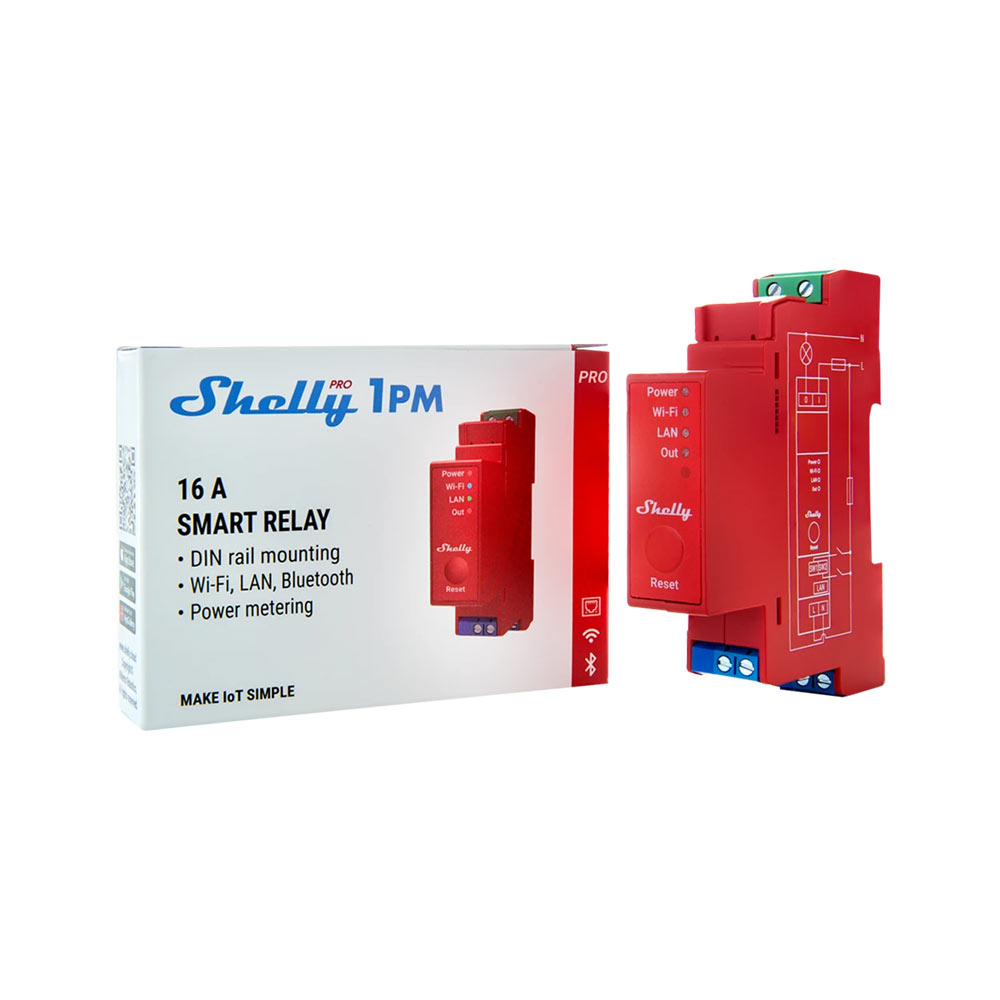
\includegraphics[width=1\textwidth]{images/Shelly-Pro-1PM-3.jpg}
  \caption{Shelly Pro 1PM}
  \label{fig:Shelly Pro 1PM}
\end{figure}

\noindent\textbf{Weitere Informationen zum Shelly Pro 1PM:} \href{https://www.shelly.com/de/products/shelly-pro-1pm}{https://www.shelly.com/de/products/shelly-pro-1pm}


Zur Steuerung wurde ein netzspannungsfähiger Shelly-Schalter zwischen Stromquelle und Dentaleinheit geschaltet. Dadurch lässt sich die Dentaleinheit gezielt über Software ein- und ausschalten – ohne physisch in die interne Steuerplatine einzugreifen. Diese Architektur bietet folgende Vorteile:
\begin{itemize}
  \item Trennung von sicherheitskritischer Hardware und externer Steuerlogik.\\
  \item Remote-Schaltung über lokale Netzwerkintegration (LAN oder WLAN).\\
  \item Einfache Erweiterbarkeit für mehrere Stühle in einer Klinik.
\end{itemize}

Shelly-Geräte zeichnen sich durch ihre vielseitige Kommunikationsfähigkeit und einfache Integration aus:
\begin{itemize}
  \item WLAN- und Bluetooth-Konnektivität.\\
  \item integrierter Webserver zur lokalen Konfiguration.\\
  \item native Unterstützung für MQTT, HTTP-API und vollständige Home Assistant-Integration.
\end{itemize}

Trotz ihrer Intelligenz und Konnektivität beeinträchtigen Shelly Smart-Schalter nicht die elektrische Integrität der angeschlossenen Geräte. Die strikte Trennung zwischen Steuer- und Lastkreis stellt sicher, dass sensible Komponenten wie die Stromversorgungsplatine der Dentaleinheit weiterhin mit der vorgesehenen Qualität und Sicherheit betrieben werden. Integrierte Schutzfunktionen wie Überspannungs-, Überstrom- und Übertemperaturschutz sowie Leistungsmessung sorgen zusätzlich für einen sicheren Betrieb.

Obwohl im Rahmen dieses Projekts Shelly-Geräte zum Einsatz kamen, ist die Lösung grundsätzlich offen für andere Smart-Schalter – sofern diese:
\begin{itemize}
  \item über vergleichbare Schutzmechanismen verfügen,\\
  \item für medizinisch-technische Umgebungen geeignet sind\\
  \item und mit Home Assistant kompatibel sind.
\end{itemize}

\subsubsection{Testaufbau mit Shelly Pro 1PM}

Zum Testen der Automatisierungslogik wurde ein einfacher Versuchsaufbau mit dem \texttt{Shelly Pro 1PM} und einem angeschlossenen \textbf{230VAC LED-Leuchtmelder} realisiert. Ziel war es, das Verhalten der geplanten Automatisierung in Home Assistant zu überprüfen, bevor der Shelly später dauerhaft zwischen die Hauptstromversorgung und das Netzteil der Dentaleinheit geschaltet wird.

\begin{figure}[H]
  \centering
  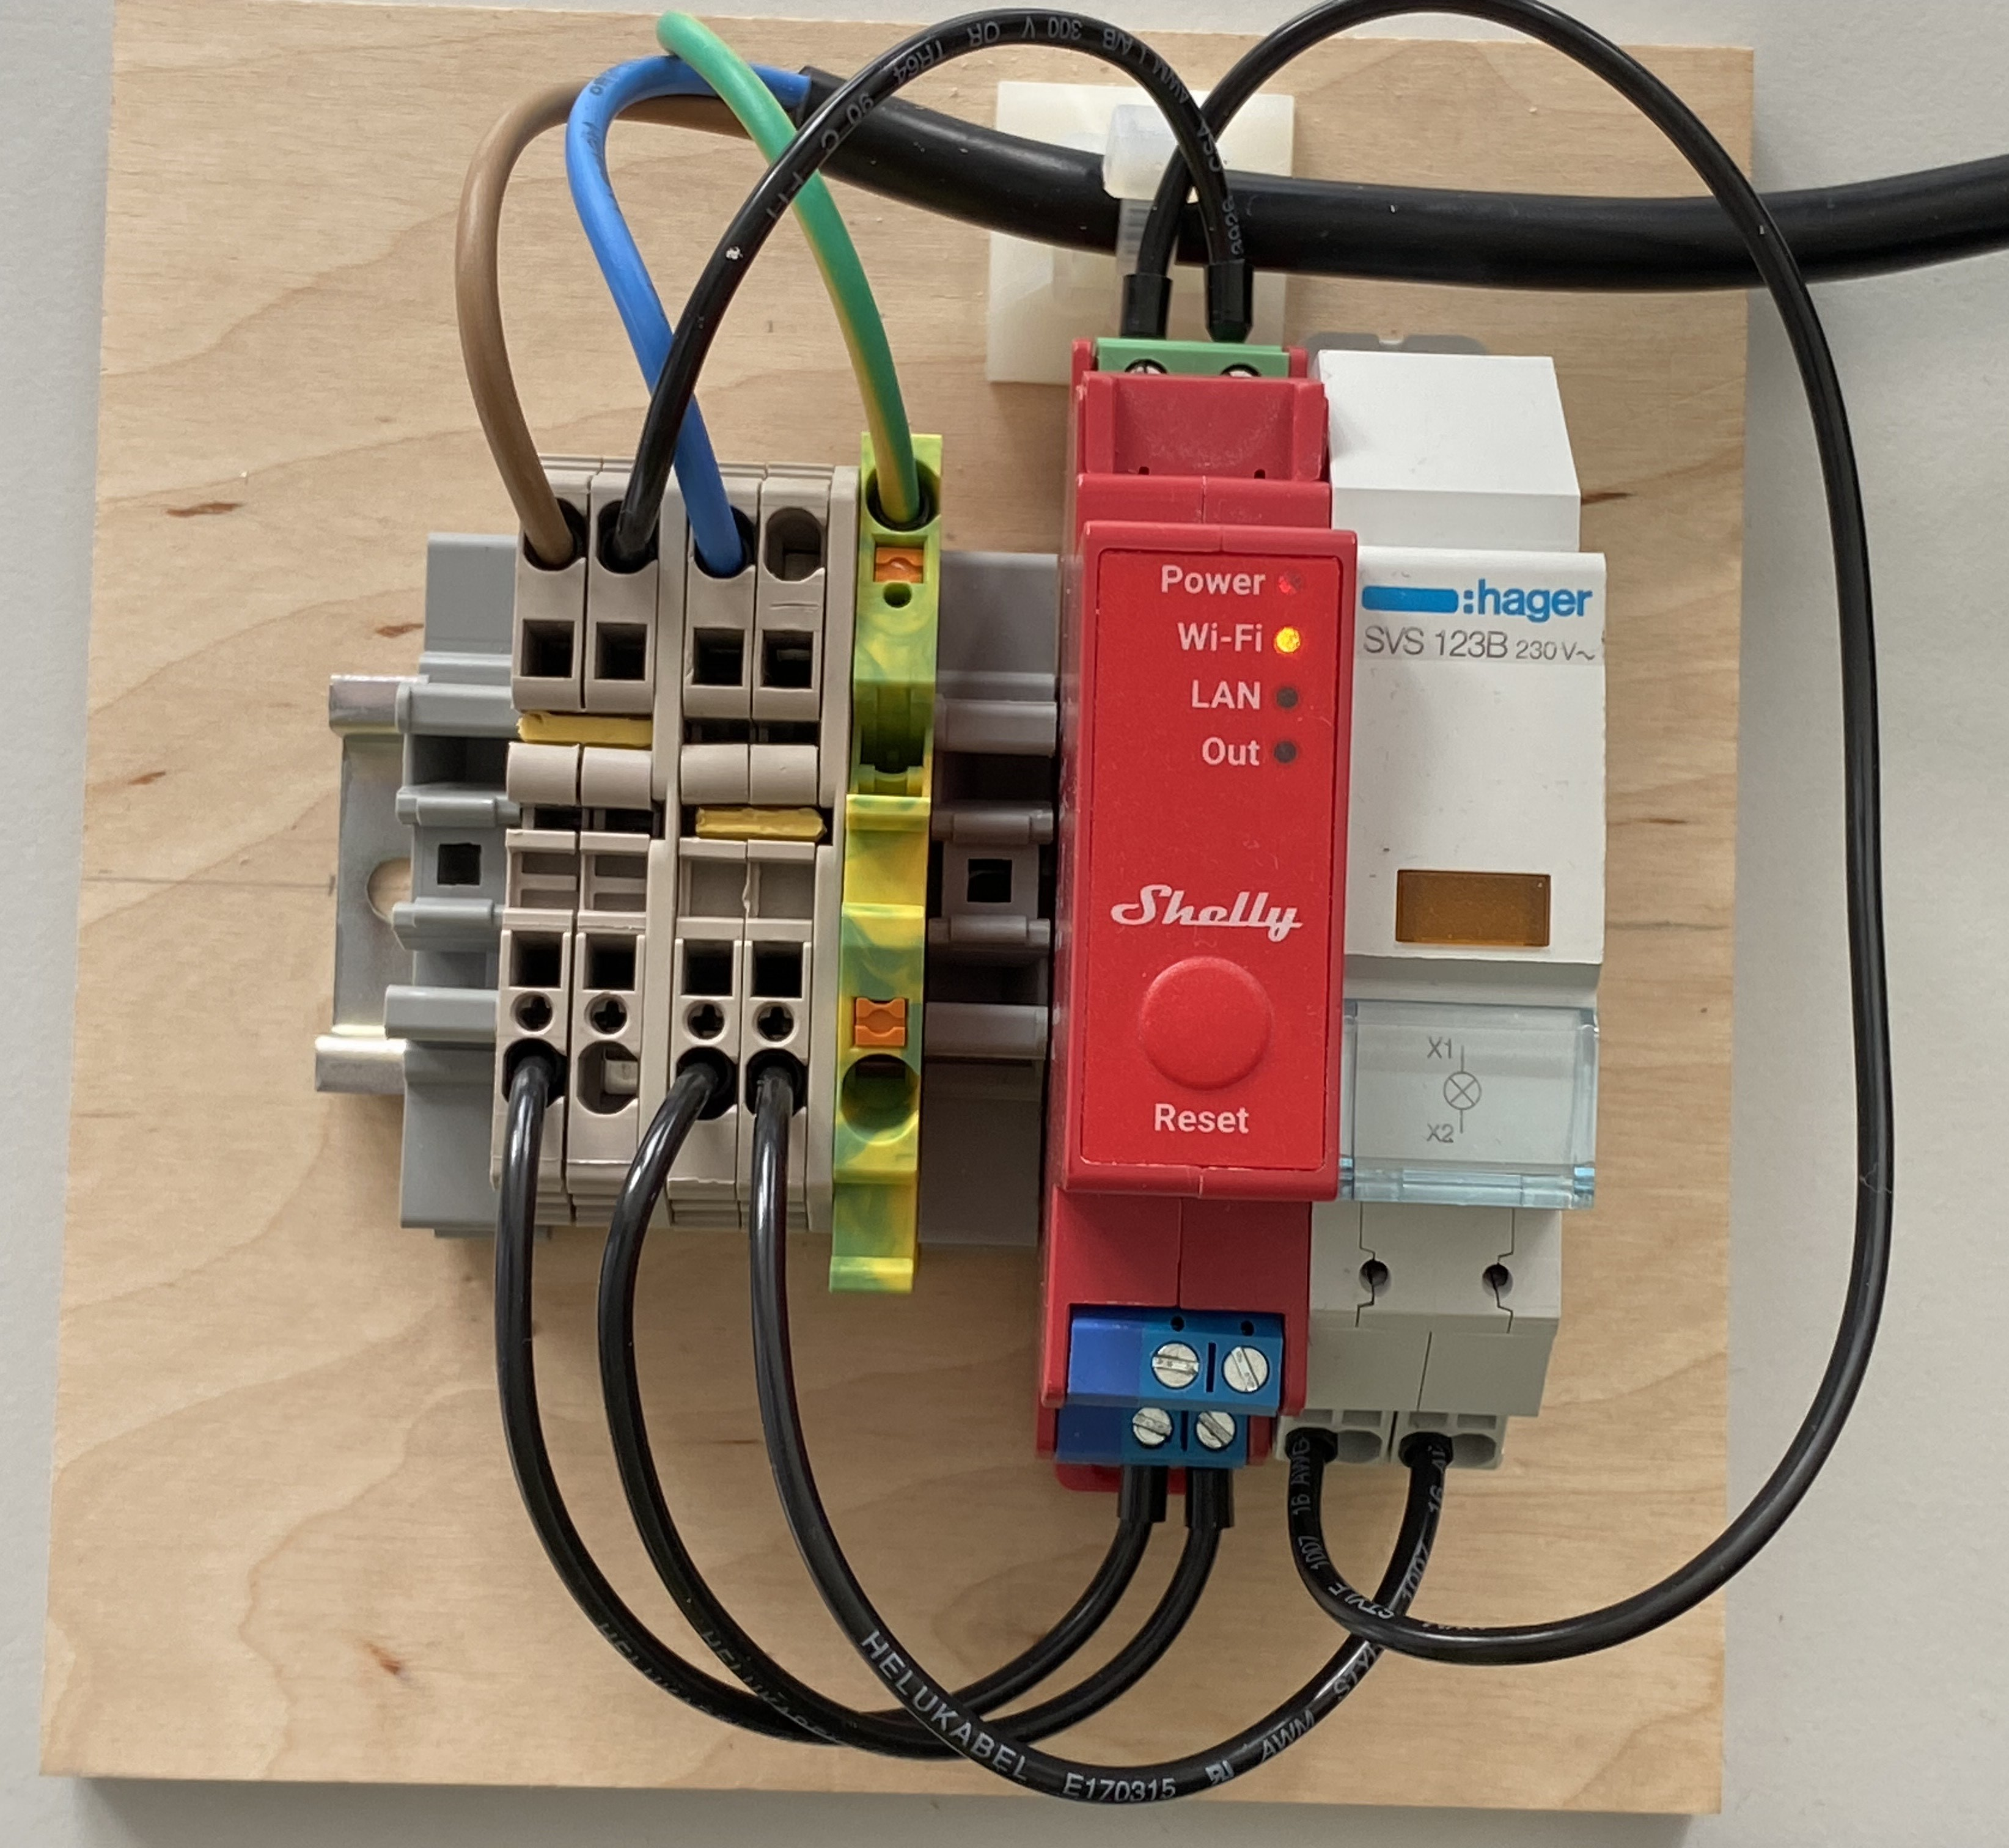
\includegraphics[width=0.6\textwidth]{images/shelly_aufbau1.jpeg}
  \caption{Testaufbau mit Shelly Pro 1PM, LED-Leuchtmelder und Klemmenblock}
  \label{fig:shelly-aufbau1}
\end{figure}

\begin{figure}[H]
  \centering
  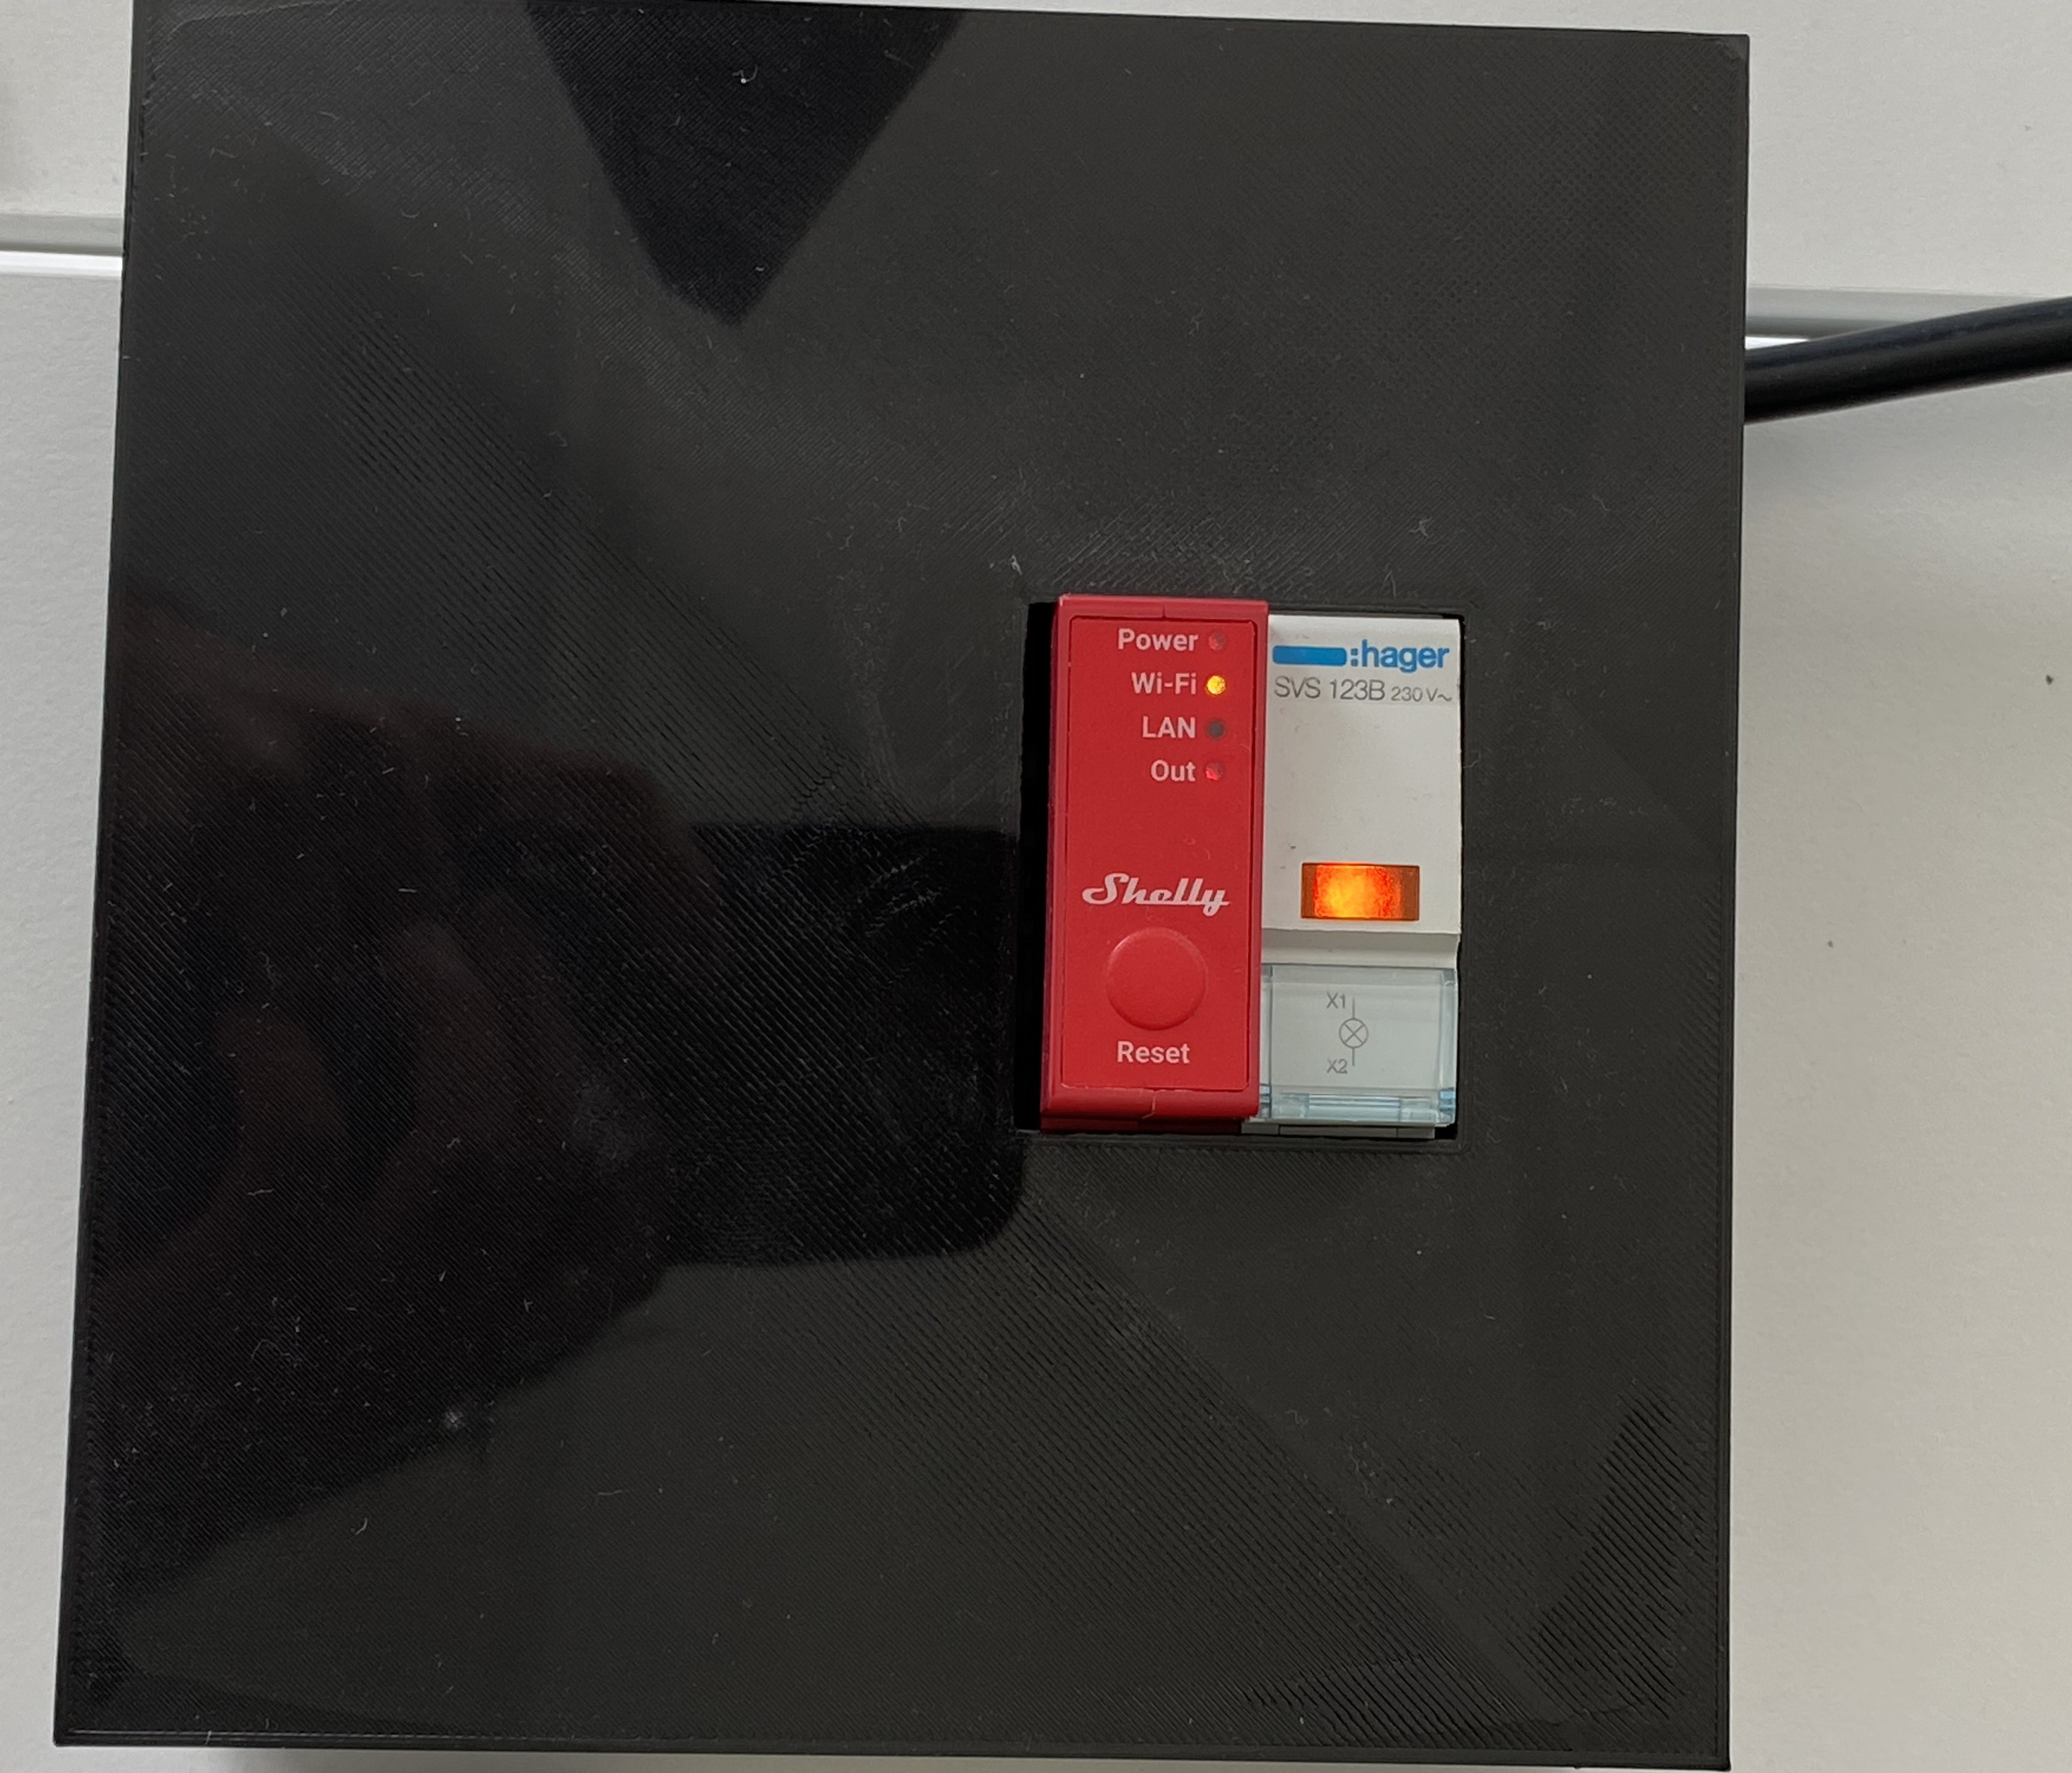
\includegraphics[width=0.6\textwidth]{images/shelly_aufbau2.jpeg}
  \caption{Abgedeckte Version des Testaufbaus}
  \label{fig:shelly-aufbau2}
\end{figure}

Der Shelly wurde über \textbf{WLAN} mit dem lokalen Netzwerk verbunden und anschließend über die Shelly-Integration in Home Assistant eingebunden.\textbf{Wichtig dabei ist, dass sich sowohl der Shelly als auch Home Assistant im selben lokalen Netzwerk befinden}. Die Schaltlogik wurde so konfiguriert, dass der Shelly den LED-Leuchtmelder mit Spannung versorgt, welcher als visueller Indikator für den Schaltzustand diente.



\subsection{Home Assistant Shelly-Integration}

Die Einrichtung der Shelly-Integration erfolgt benutzerfreundlich über die grafische Oberfläche von Home Assistant. Unter \texttt{Einstellungen > Geräte \& Dienste} kann mit dem Button \texttt{Integration hinzufügen} nach „Shelly“ gesucht und die Integration mit wenigen Klicks installiert werden:

\begin{figure}[H]
  \centering
  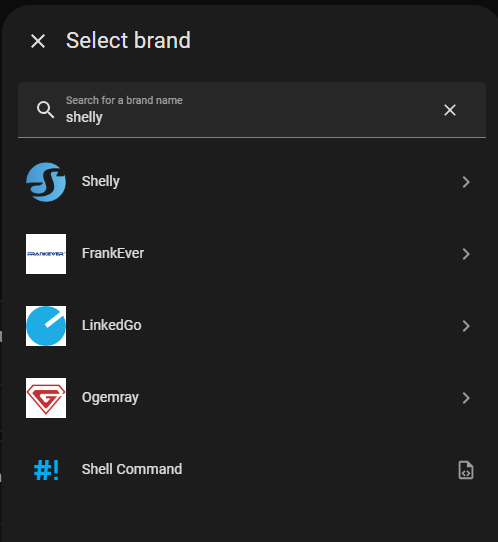
\includegraphics[width=0.65\linewidth]{images/add_shelly_integration.png}
  \caption{Shelly-Integration über die Home Assistant Benutzeroberfläche hinzufügen}
\end{figure}

Die Integration von Shelly-Geräten in Home Assistant erfolgt nahtlos über die offizielle Shelly-Integration oder über MQTT. Dabei werden automatisch Steuer- und Statusentitäten erzeugt, unter anderem:
\begin{itemize}
  \item \textbf{Switch-Entität:} Ermöglicht das Ein- und Ausschalten über die Benutzeroberfläche, Automationen oder Kalendereinträge.\\
  \item \textbf{Leistungsmessung:} Die aktuelle Leistungsaufnahme kann überwacht und in Automatisierungen einbezogen werden.\\
  \item \textbf{Zustandsentitäten:} Übermitteln den Verbindungsstatus und eventuelle Fehlfunktionen.\\
\end{itemize}

\begin{figure}[H]
  \centering
  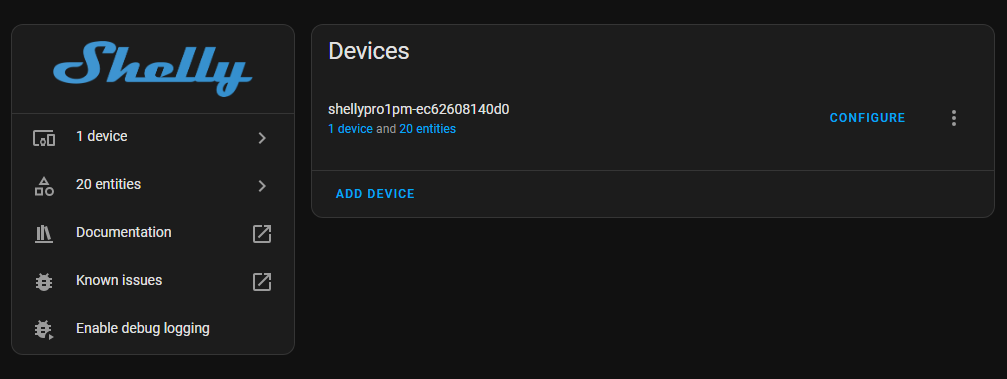
\includegraphics[width=1\linewidth]{images/ha_shelly}
  \caption{Einbindung des Shelly Pro 1PM in Home Assistant}
\end{figure}

\begin{figure}[H]
  \centering
  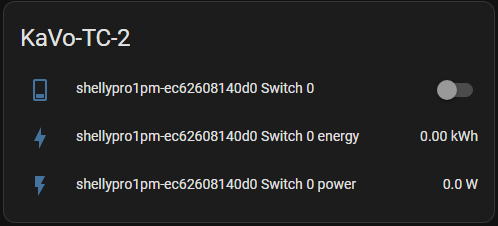
\includegraphics[width=0.65\linewidth]{images/ha_shelly_2.png}
  \caption{Automatisch erkannte Entitäten für \texttt{KaVo-TC-2}(Shelly Pro 1PM von diese Dentaleinheit)}
\end{figure}

\subsection{Automatisierung über Home Assistant}

Für dieses Projekt wurde eine Automation in Home Assistant implementiert, die den \texttt{Shelly Pro 1PM} automatisch \emph{eine Minute vor Beginn} eines geplanten Hygieneprogramms einschaltet und ihn nach Abschluss der abendlichen oder wöchentlichen Reinigungsphase wieder deaktiviert. Die zugrundeliegenden Kalendereinträge und Entitäten werden dabei direkt über WebSocket von der Dentaleinheit an Home Assistant übermittelt. Dies ermöglicht eine fehlerfreie und synchronisierte Steuerung der Stromzufuhr – ganz ohne manuelle Eingriffe.

Die Idee hinter dieser Architektur ist es, alle relevanten Entitäten, die für Automationen benötigt werden, durch die \textbf{eigene KaVo Home Assistant-Integration} verfügbar zu machen. Dazu zählen unter anderem Kalender-, Sensor- und Statusentitäten, die den Zustand des Hygieneplans oder der Verbindung zum Stuhl abbilden.

Die IT-Abteilung oder technische Betreuung der jeweiligen Zahnarztpraxis kann auf dieser Grundlage eigene Automationen direkt in der intuitiven Benutzeroberfläche von Home Assistant erstellen. Dafür stehen alle Entitäten der verbundenen KaVo-Einheiten bereit. 

\begin{itemize}
  \item Es wurden exemplarisch mehrere Automationen erstellt, die direkt wiederverwendet werden können, um die Ein- und Ausschaltung des Schalters basierend auf Hygieneplan-Zeitpunkten zu steuern.\\
  \item Gleichzeitig bleibt volle Flexibilität: Durch das einfache UI können individuelle Zeitpläne, Reaktionsbedingungen und Benachrichtigungsfunktionen ohne Programmierkenntnisse konfiguriert werden.
\end{itemize}

\subsubsection{Automationplans Overview}

Zur Übersicht zeigt Abbildung~\ref{fig:automation_overview} die drei entwickelten Automationslogiken für die Steuerung des Shelly Pro 1PM.

\begin{figure}[H]
  \centering
  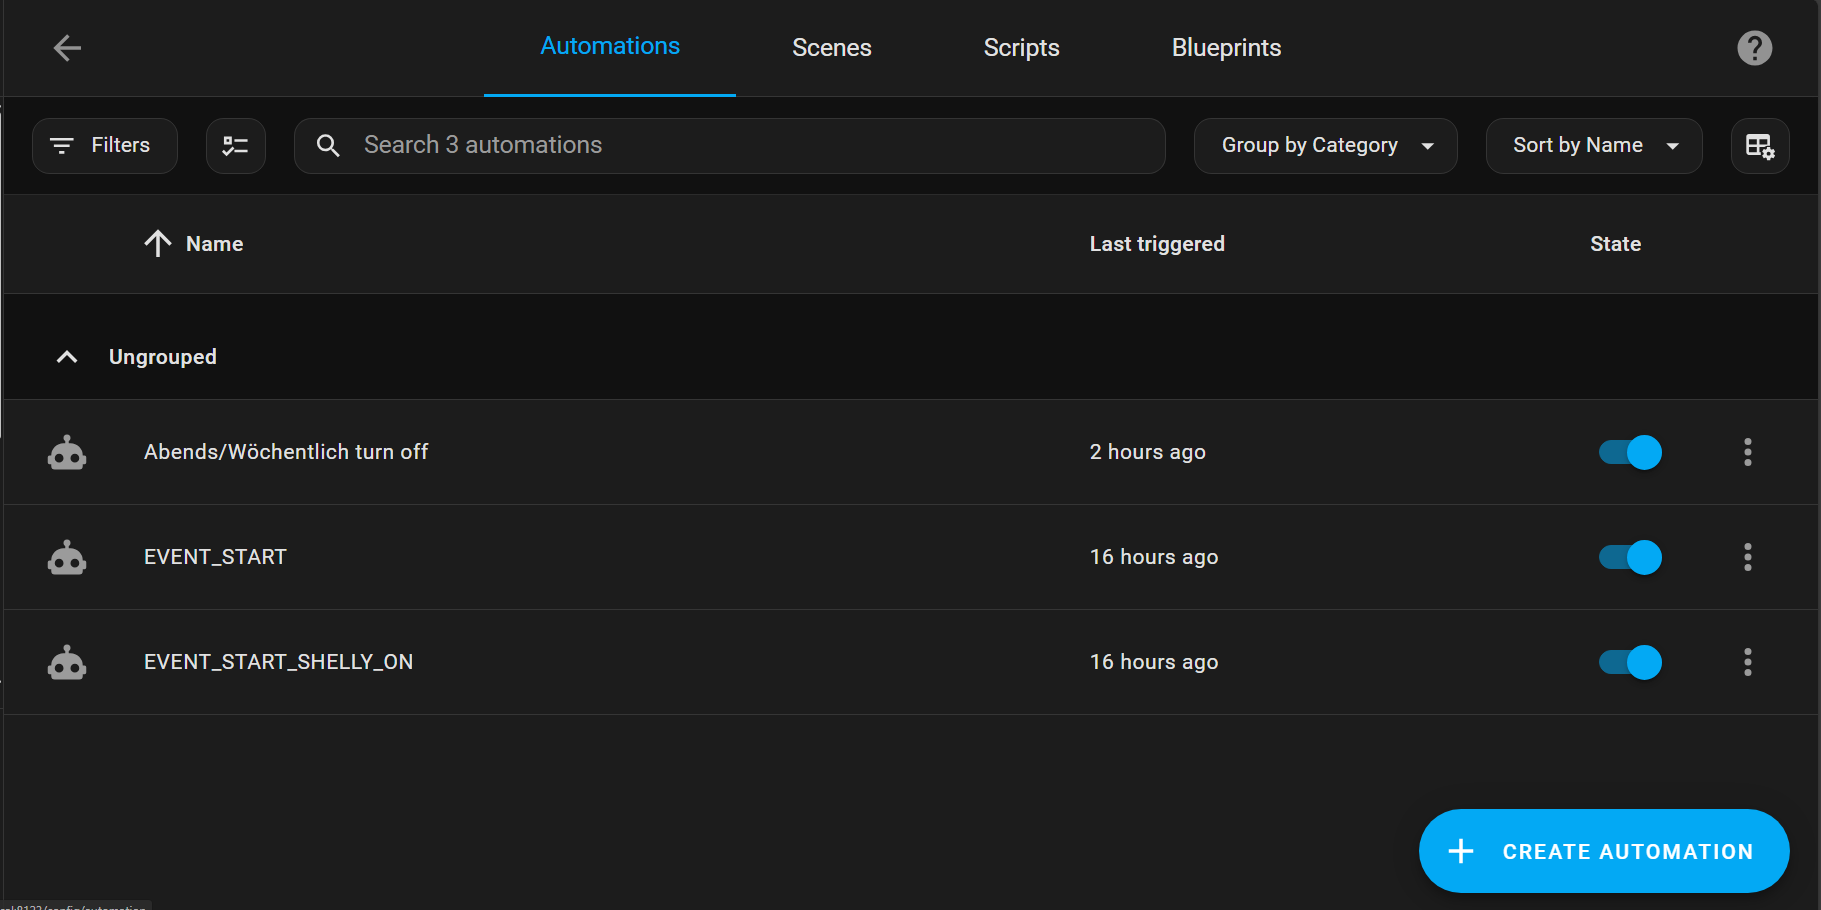
\includegraphics[width=\linewidth]{images/Automation_overview.png}
  \caption{Übersicht der Automationspläne in Home Assistant}
  \label{fig:automation_overview}
\end{figure}

\subsubsection{Abends/Wöchentlich Turn Off}

Diese Automation schaltet den \texttt{Shelly Pro 1PM} automatisch aus, nachdem die abendliche oder wöchentliche Hygiene abgeschlossen wurde. Die Logik basiert auf der Änderung des Status der Entität \texttt{sensor.kavo\_tc\_2\_hygiene\_plan\_phase}.

\begin{figure}[H]
  \centering
  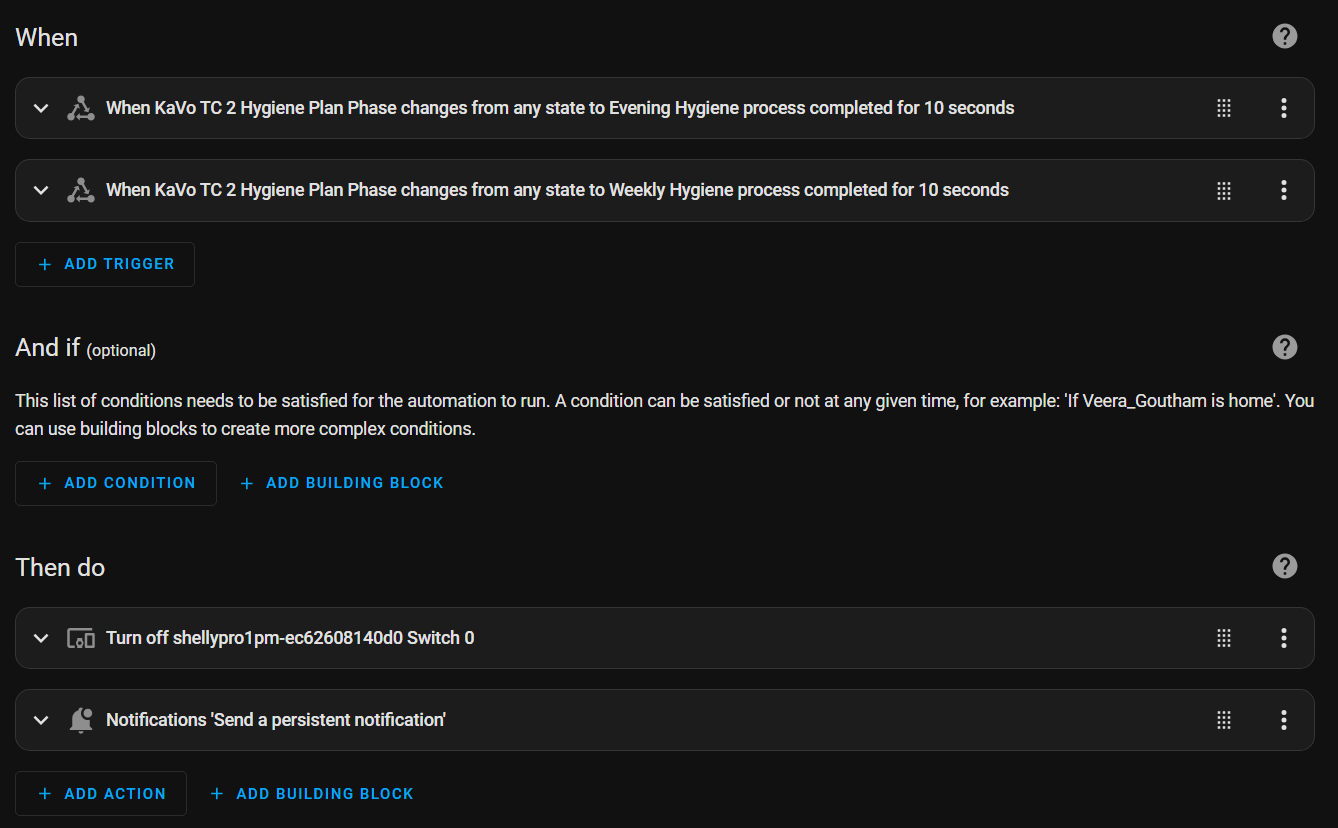
\includegraphics[width=\linewidth]{images/turnoff_overview.png}
  \caption{Automation-Übersicht: Abends/Wöchentlich}
\end{figure}

\begin{figure}[H]
  \centering
  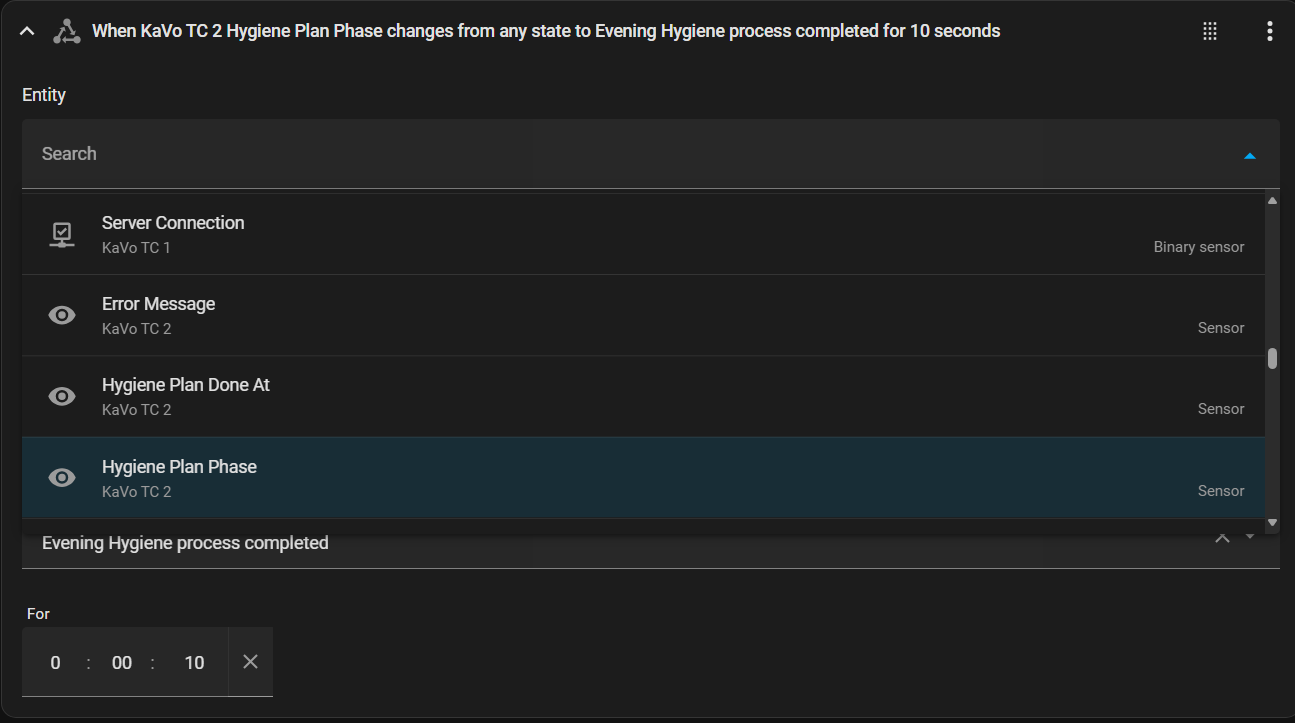
\includegraphics[width=\linewidth]{images/turnoff_triggerentity.png}
  \caption{Entitätsauswahl für Status-Trigger}
\end{figure}

\begin{figure}[H]
  \centering
  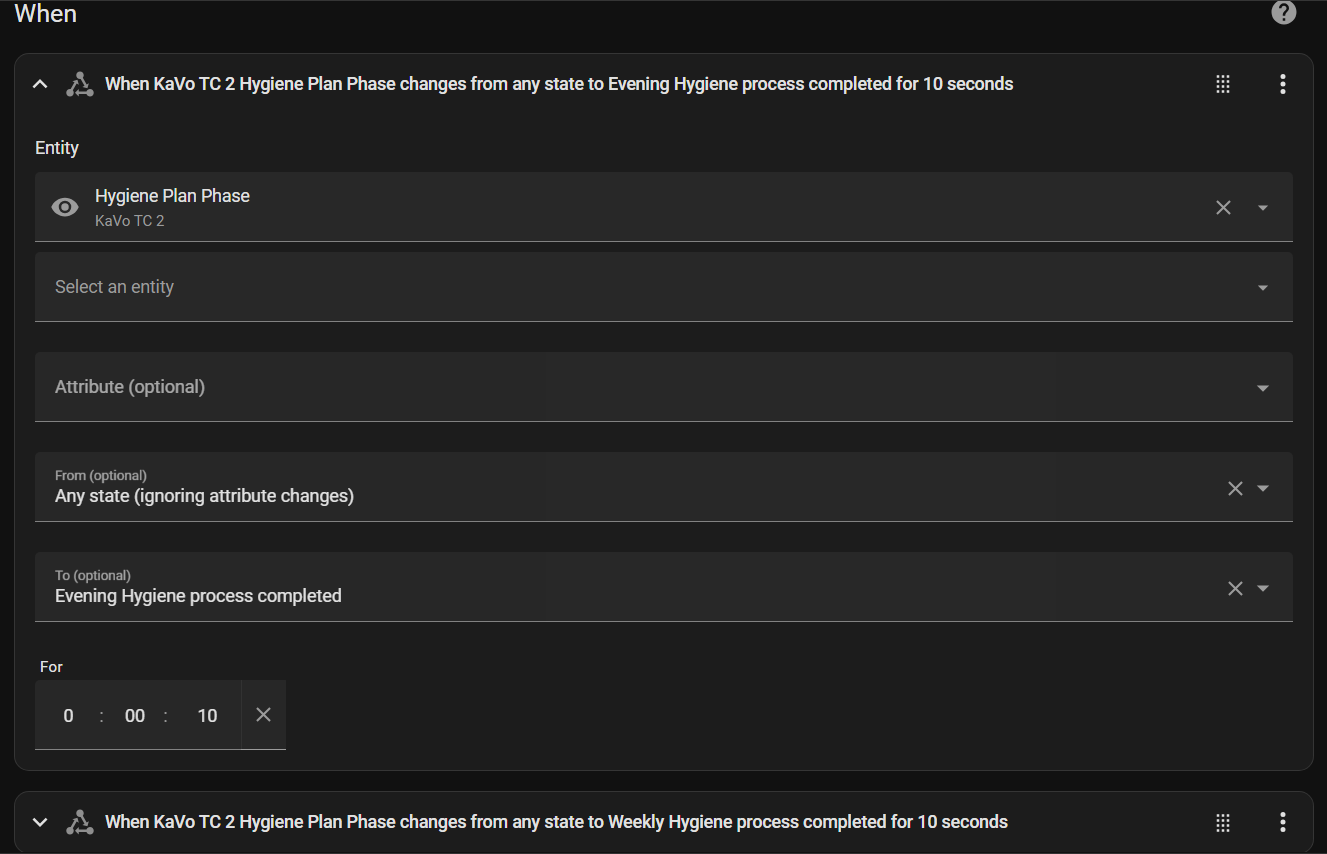
\includegraphics[width=\linewidth]{images/turnoff_trigger.png}
  \caption{Trigger: Statusänderung in Hygiene Plan Phase}
\end{figure}

\begin{figure}[H]
  \centering
  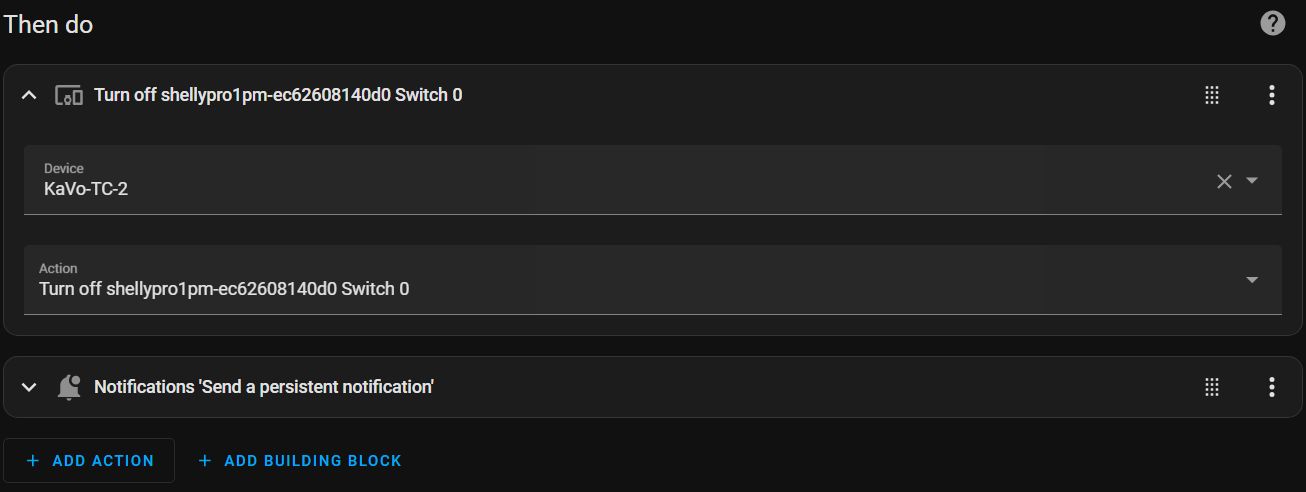
\includegraphics[width=\linewidth]{images/turnoff_action.png}
  \caption{Aktionen nach Trigger: Shelly ausschalten}
\end{figure}

\begin{figure}[H]
  \centering
  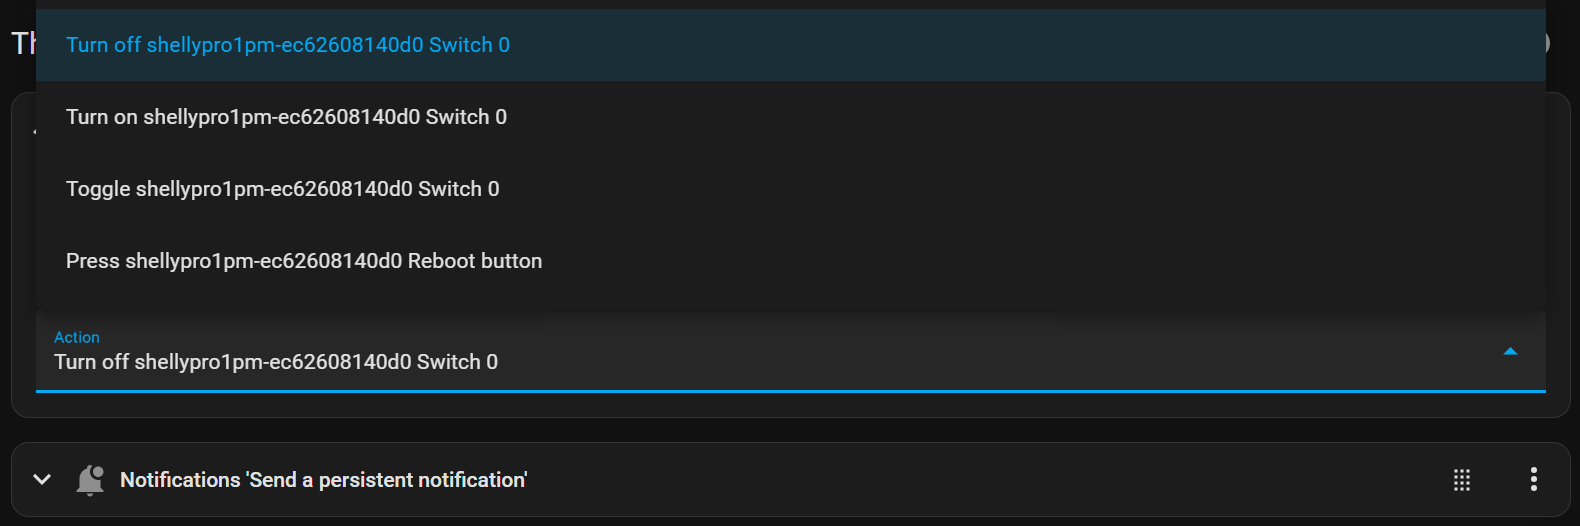
\includegraphics[width=\linewidth]{images/turnoff_actions.png}
  \caption{Verfügbare Aktionen}
\end{figure}

\subsubsection{EVENT\_START\_SHELLY\_ON}

Diese Automation schaltet den \texttt{Shelly Pro 1PM} eine Minute vor dem Start eines geplanten Hygieneprogramms ein. Der Startzeitpunkt wird aus dem Kalendereintrag der Dentaleinheit übernommen.

\begin{figure}[H]
  \centering
  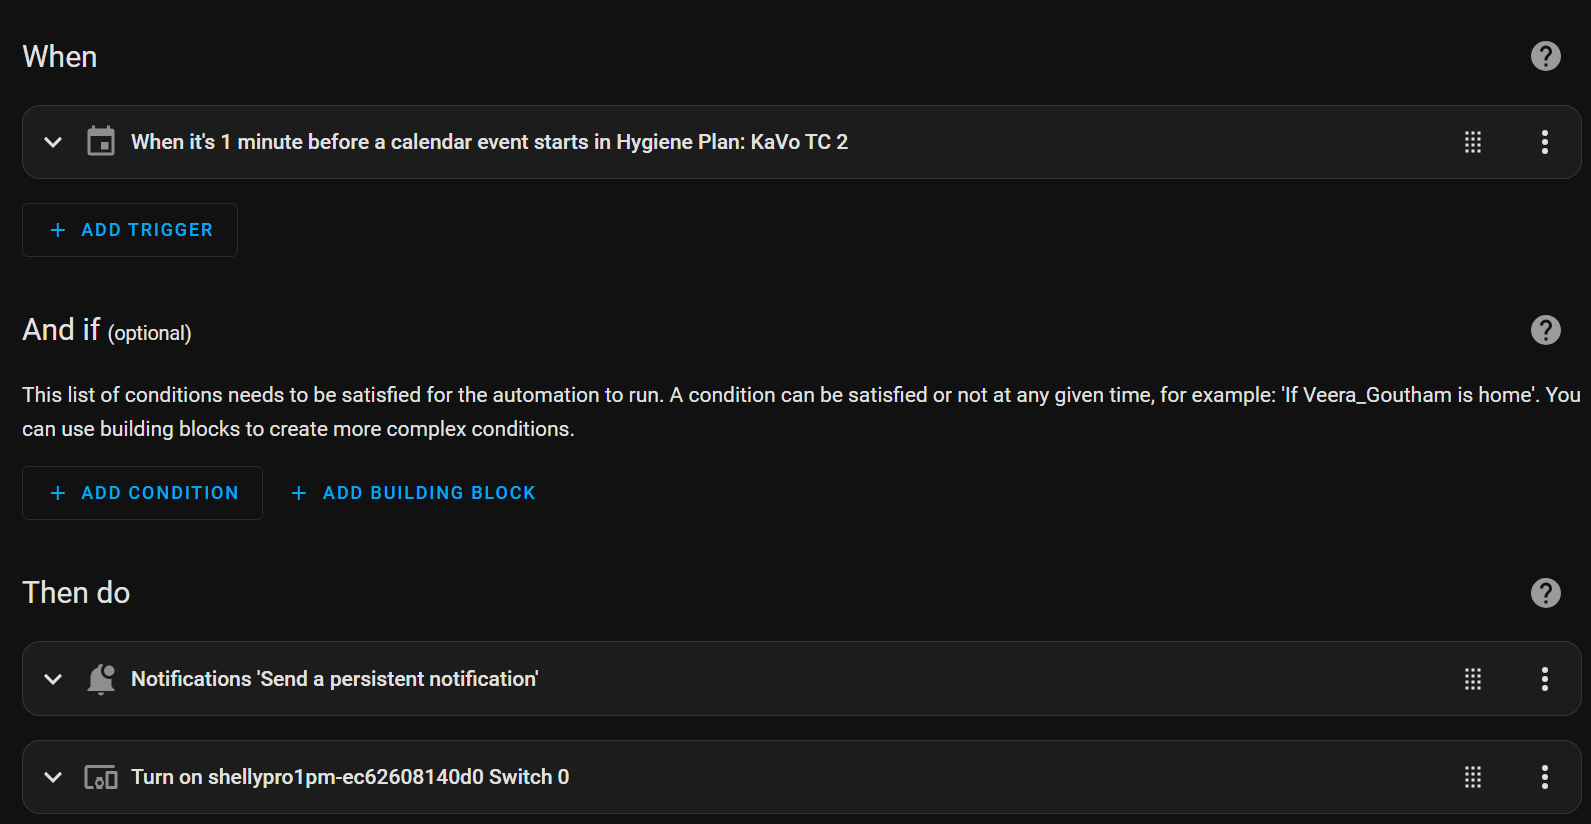
\includegraphics[width=\linewidth]{images/turnon_overview.png}
  \caption{Automation-Übersicht: EVENT\_START\_SHELLY\_ON}
\end{figure}

\begin{figure}[H]
  \centering
  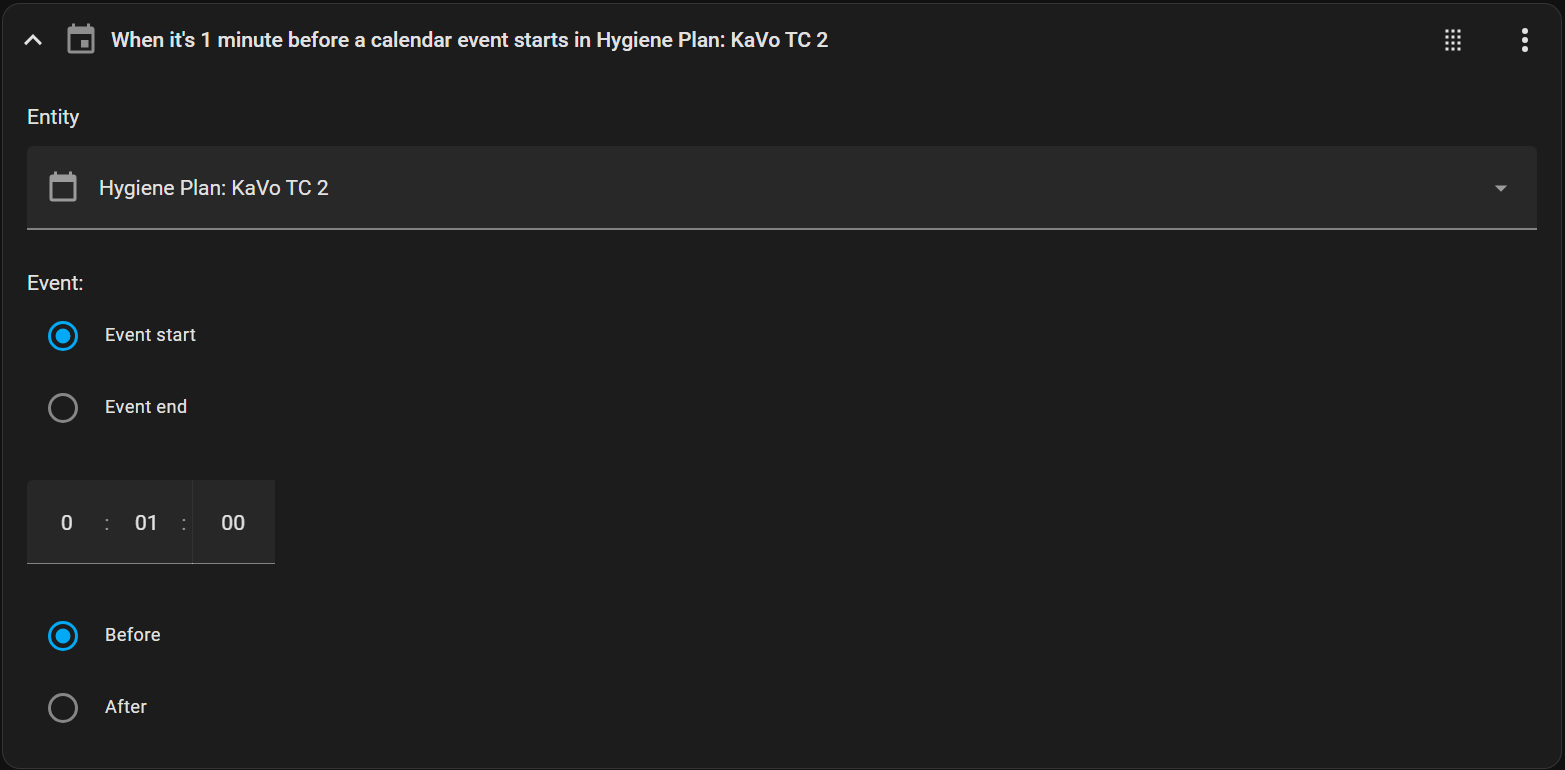
\includegraphics[width=\linewidth]{images/turnon_trigger.png}
  \caption{Trigger: Kalendereintrag startet (Offset -1 Minute)}
\end{figure}


Diese Lösung bietet nicht nur eine praxisnahe Automatisierungsvorlage, sondern ermöglicht auch maximale Anpassungsfreiheit und Skalierbarkeit für unterschiedlichste Anwendungsszenarien in Zahnarztpraxen.




